%%%%%%%%%%%%%%%%%%%%%%%%%%%%%%%%%%%%%%%%%%%%%%%%%%%%%%%%%%%%%%%
%% OXFORD THESIS TEMPLATE

% Use this template to produce a standard thesis that meets the Oxford University requirements for DPhil submission
%
% Originally by Keith A. Gillow (gillow@maths.ox.ac.uk), 1997
% Modified by Sam Evans (sam@samuelevansresearch.org), 2007
% Modified by John McManigle (john@oxfordechoes.com), 2015
%GArextraprops
% This version Copyright (c) 2015-2023 John McManigle
%
% Broad permissions are granted to use, modify, and distribute this software
% as specified in the MIT License included in this distribution's LICENSE file.
%

% I've (John) tried to comment this file extensively, so read through it to see how to use the various options.  Remember
% that in LaTeX, any line starting with a % is NOT executed.  Several places below, you have a choice of which line to use
% out of multiple options (eg draft vs final, for PDF vs for binding, etc.)  When you pick one, add a % to the beginning of
% the lines you don't want.


%%%%% CHOOSE PAGE LAYOUT
% The most common choices should be below.  You can also do other things, like replacing "a4paper" with "letterpaper", etc.

% This one will format for two-sided binding (ie left and right pages have mirror margins; blank pages inserted where needed):
\documentclass[a4paper,twoside]{ociamthesis}
% This one will format for one-sided binding (ie left margin > right margin; no extra blank pages):
%\documentclass[a4paper]{ociamthesis}
% This one will format for PDF output (ie equal margins, no extra blank pages):
%\documentclass[a4paper,nobind]{ociamthesis} 



%%%%% SELECT YOUR DRAFT OPTIONS
% Three options going on here; use in any combination.  But remember to turn the first two off before
% generating a PDF to send to the printer!

% This adds a "DRAFT" footer to every normal page.  (The first page of each chapter is not a "normal" page.)
\fancyfoot[C]{\emph{DRAFT Printed on \today}}  

% This highlights (in blue) corrections marked with (for words) \mccorrect{blah} or (for whole
% paragraphs) \begin{mccorrection} . . . \end{mccorrection}.  This can be useful for sending a PDF of
% your corrected thesis to your examiners for review.  Turn it off, and the blue disappears.
\correctionstrue


%%%%% BIBLIOGRAPHY SETUP
% Note that your bibliography will require some tweaking depending on your department, preferred format, etc.
% The options included below are just very basic "sciencey" and "humanitiesey" options to get started.
% If you've not used LaTeX before, I recommend reading a little about biblatex/biber and getting started with it.
% If you're already a LaTeX pro and are used to natbib or something, modify as necessary.
% Either way, you'll have to choose and configure an appropriate bibliography format...

% The science-type option: numerical in-text citation with references in order of appearance.
\usepackage[style=numeric-comp, sorting=none, backend=biber, doi=false, isbn=false]{biblatex}
\newcommand*{\bibtitle}{References}

% The humanities-type option: author-year in-text citation with an alphabetical works cited.
%\usepackage[style=authoryear, sorting=nyt, backend=biber, maxcitenames=2, useprefix, doi=false, isbn=false]{biblatex}
%\newcommand*{\bibtitle}{Works Cited}

% This makes the bibliography left-aligned (not 'justified') and slightly smaller font.
\renewcommand*{\bibfont}{\raggedright\small}

% Change this to the name of your .bib file (usually exported from a citation manager like Zotero or EndNote).
\addbibresource{references.bib}

% Uncomment this if you want equation numbers per section (2.3.12), instead of per chapter (2.18):
%\numberwithin{equation}{subsection}
\usepackage{subcaption}
%\captionsetup[subfigure]{labelformat=empty}



%%%%% THESIS / TITLE PAGE INFORMATION
% Everybody needs to complete the following:
\title{Neutrino Interactions with a High-Pressure Gas Time Projection Chamber}
\author{Federico Battisti}
\college{Pembroke College}

% Master's candidates who require the alternate title page (with candidate number and word count)
% must also un-comment and complete the following three lines:
%\masterssubmissiontrue
%\candidateno{933516}
%\wordcount{28,815}

% Uncomment the following line if your degree also includes exams (eg most masters):
%\renewcommand{\submittedtext}{Submitted in partial completion of the}
% Your full degree name.  (But remember that DPhils aren't "in" anything.  They're just DPhils.)
\degree{Doctor of Philosophy}
% Term and year of submission, or date if your board requires (eg most masters)
\degreedate{Michaelmas 2024}


%%%%% YOUR OWN PERSONAL MACROS
% This is a good place to dump your own LaTeX macros as they come up.

% To make text superscripts shortcuts
	\renewcommand{\th}{\textsuperscript{th}} % ex: I won 4\th place
	\newcommand{\nd}{\textsuperscript{nd}}
	\renewcommand{\st}{\textsuperscript{st}}
	\newcommand{\rd}{\textsuperscript{rd}}

%%%%% THE ACTUAL DOCUMENT STARTS HERE
\begin{document}



%%%%% CHOOSE YOUR LINE SPACING HERE
% This is the official option.  Use it for your submission copy and library copy:
\setlength{\textbaselineskip}{22pt plus2pt}
% This is closer spacing (about 1.5-spaced) that you might prefer for your personal copies:
%\setlength{\textbaselineskip}{18pt plus2pt minus1pt}

% You can set the spacing here for the roman-numbered pages (acknowledgements, table of contents, etc.)
\setlength{\frontmatterbaselineskip}{17pt plus1pt minus1pt}

% Leave this line alone; it gets things started for the real document.
\setlength{\baselineskip}{\textbaselineskip}


%%%%% CHOOSE YOUR SECTION NUMBERING DEPTH HERE
% You have two choices.  First, how far down are sections numbered?  (Below that, they're named but
% don't get numbers.)  Second, what level of section appears in the table of contents?  These don't have
% to match: you can have numbered sections that don't show up in the ToC, or unnumbered sections that
% do.  Throughout, 0 = chapter; 1 = section; 2 = subsection; 3 = subsubsection, 4 = paragraph...

% The level that gets a number:
\setcounter{secnumdepth}{2}
% The level that shows up in the ToC:
\setcounter{tocdepth}{2}


%%%%% ABSTRACT SEPARATE
% This is used to create the separate, one-page abstract that you are required to hand into the Exam
% Schools.  You can comment it out to generate a PDF for printing or whatnot.
\begin{abstractseparate}
	Your abstract text goes here.  Check your departmental regulations, but generally this should be less than 300 words.  See the beginning of Chapter~\ref{ch:2-litreview} for more.
 % Create an abstract.tex file in the 'text' folder for your abstract.
\end{abstractseparate}


% JEM: Pages are roman numbered from here, though page numbers are invisible until ToC.  This is in
% keeping with most typesetting conventions.
\begin{romanpages}

% JEM: By default, this template uses the traditional Oxford "Belt Crest". Un-comment the following
% line to use the newer, "Blue Square" logo:
% \renewcommand{\crest}{{\includegraphics[width=4.2cm, height=4.2cm]{figures/newlogo.pdf}}}

% Title page is created here
\maketitle

%%%%% DEDICATION -- If you'd like one, un-comment the following.
%\begin{dedication}
%This thesis is dedicated to\\
%someone\\
%for some special reason\\
%\end{dedication}

%%%%% ACKNOWLEDGEMENTS -- Nothing to do here except comment out if you don't want it.
\begin{acknowledgements}
 	

\end{acknowledgements}

%%%%% ABSTRACT -- Nothing to do here except comment out if you don't want it.
\begin{abstract}
	Your abstract text goes here.  Check your departmental regulations, but generally this should be less than 300 words.  See the beginning of Chapter~\ref{ch:2-litreview} for more.

\end{abstract}

%%%%% MINI TABLES
% This lays the groundwork for per-chapter, mini tables of contents.  Comment the following line
% (and remove \minitoc from the chapter files) if you don't want this.  Un-comment either of the
% next two lines if you want a per-chapter list of figures or tables.
\dominitoc % include a mini table of contents
%\dominilof  % include a mini list of figures
%\dominilot  % include a mini list of tables

% This aligns the bottom of the text of each page.  It generally makes things look better.
\flushbottom

% This is where the whole-document ToC appears:
\tableofcontents

\listoffigures
	\mtcaddchapter
% \mtcaddchapter is needed when adding a non-chapter (but chapter-like) entity to avoid confusing minitoc

% Uncomment to generate a list of tables:
%\listoftables
%	\mtcaddchapter

%%%%% LIST OF ABBREVIATIONS
% This example includes a list of abbreviations.  Look at text/abbreviations.tex to see how that file is
% formatted.  The template can handle any kind of list though, so this might be a good place for a
% glossary, etc.
% First parameter can be changed eg to "Glossary" or something.
% Second parameter is the max length of bold terms.
\begin{mclistof}{List of Abbreviations}{3.2cm}

\item[1-D, 2-D] One- or two-dimensional, referring in this thesis to spatial dimensions in an image.


\end{mclistof} 


% The Roman pages, like the Roman Empire, must come to its inevitable close.
\end{romanpages}


%%%%% CHAPTERS
% Add or remove any chapters you'd like here, by file name (excluding '.tex'):
\flushbottom
\begin{savequote}[8cm]
\end{savequote}

\chapter*{\label{ch:1-intro}Introduction} 
\minitoc

The Deep Underground Neutrino Experiment (DUNE) \cite{DUNE:2020TDR1} will be a new generation accelerator oscillation neutrino experiment. It will include three main components: a powerful wide-band neutrino beam situated at Fermilab, a multi-instrumented Near Detector positioned a few hundred meters from the neutrino source and a Far Detector situated 1300 km away from the source in South Dakota. The key goal of the DUNE experiment will be to initiate a new era of precision in the field of neutrino flavour oscillations by performing a complete range of measurements using both neutrino and antineutrino beams. Particular emphasis will be put on the measurement of charge parity violation in neutrino oscillations and determining the order of the neutrino mass eigenstates.

In order to perform neutrino oscillation measurements, a prediction for the expected signal and background at the Far Detector as a function of the oscillation parameters, needs to be produced. The prediction is then compared with the measured flavor-tagged neutrino spectra at the Far Detector,
in order to produce estimates for the parameters that regulate the oscillation probability. Producing this prediction requires the determination of the neutrino flux at production, the neutrino interaction cross sections and the response of the detector: all of these factors are affected by systematic uncertainties that need to be constrained. The DUNE Near Detector has been designed to specifically
address each element \cite{DUNE:2021NDCDR}.

The DUNE ND will include as one of its main components a high pressure gas time projection chamber (HpGTPC) based on Argon called ND-GAr. The TPC technology has enjoyed ample success in high-energy particle physics. Since its original proposal by Nygren in 1975~\cite{NygrenTPC}, it has been utilized in various experiments and setups ~\cite{ATTIE200989,Hilke:2010zz}. One of the most notable examples of gas TPC's in modern particle physics is the ALICE experiment at CERN~\cite{ALICE:2008ngc}. The design of ND-GAr is heavily inspired by ALICE, to the point that the multi-wire proportional chambers that will be used by ND-GAr will be repurposed from the ALICE detector after its recent upgrade~\cite{ALICE:2023udb}. The use of a gas TPC in a neutrino experiment is unprecedented and it is motivated by the low tracking thresholds and extreme levels of precision achievable using this technology. These features will be particularly useful in the study of neutrino interactions and nuclear effects, which are one of the key sources of systematic uncertainty in the oscillation measurement.

In this thesis we present the conception, development and testing of what is now the standard momentum reconstruction algorithm used by the TPC component of the ND-GAr detector. The algorithm is based on the Kalman Filter technique, which is an iterative Bayesian technique often used in the field of particle tracking. This Kalman Filter application presents some novel features which allow it to reconstruct very long low energy tracks, which is particularly beneficial to a neutrino experiment such as ND-GAr. The method was developed in collaboration with experts of the ALICE collaboration and is envisioned to be used by both experiments. A similar more simple algorithm was also developed for ND-GAr-Lite, a now abandoned temporary muon spectrometer design centered on a multi-layer scintillator tracker,that would have substituted ND-GAr in the early days of the experiment's lifetime.

The impact of this novel Kalman Filter was tested in a significant physics application: as already mentioned, one of the key roles of the ND-GAr detector will be to act as a laboratory for the study of nuclear effects in neutrino interactions. One of the key techniques that will be used by the experiment is transverse kinematic imbalance (TKI)~\cite{Lu:2015hea, PhysRevC.94.015503, PhysRevC.99.055504, Cai:2019jzk, PhysRevD.102.033005}, a method inspired by the missing energy concept in high energy physics. It has been suggested that TKI could be used in a HpgTPC to isolate a sample of neutrino-Hydrogen interactions present in the gas mixture. Hydrogen interactions are devoid of nuclear effects and represents an ideal testing ground for the characterization of these crucial systematic uncertainty sources. The efficacy of the technique is in large part determined by the resolution of the detector, making the impact of the novel Kalman Filter very directly detectable.

This thesis is structured as follows:
\begin{itemize}
    \item Chapter \ref{ch:2-litreview} offers an introduction to neutrino physics and some key experimental particle physics concepts.
    \item Chapter \ref{ch:3-DUNE} provides a description of the DUNE experiment and its physics goals, with particular focus on the Near Detector and ND-GAr.
    \item Chapter \ref{ch:4-KF-NDGArLite} introduces the key concepts behind the Kalman Filter technique and offers a description of a Kalman Filter application developed for the ND-GAr-Lite temporary muon spectrometer.
    \item Chapter \ref{ch:5-KF-NDGArToy} introduces the novel Kalman Filter developed for the ND-GAr detector and investigates its performance.
    \item Chapter \ref{ch:6-TKI} describes a study on the capability of the ND-GAr detector of using transverse kinematic imbalance to isolate a sample of neutrino-Hydrogen interactions, exploring the impact of the new Kalman Filter algorithm.
\end{itemize}









\begin{savequote}[8cm]
Ci sono soltanto due possibili conclusioni: \\
se il risultato conferma l'ipotesi,\\
allora hai appena fatto una misura. \\
Se il risultato è contrario alle ipotesi, \\
allora hai fatto una scoperta.

There are only two possible conclusions:\\
if the result confirms the hypothesis, \\
then you made a measurement.\\
If the result contradicts the hypothesis, \\
then you made a discovery.
  \qauthor{--- Enrico Fermi}
\end{savequote}

\chapter{\label{ch:2-litreview}Theoretical Background}
\minitoc
\section{Brief history of neutrinos}
\section{Neutrino in the Standard Model and neutrino masses}
\section{Theory of neutrino Oscillations}
\subsection{Two flavour scenario}
\subsection{Three flavour Oscillation in vacuum}
\subsection{Charge-Parity Simmetry Violation}
\subsection{Mass-Hierarchy}
\subsection{MSW effect}
\section{Neutrino Oscillation Experiments}
\subsection{Solar Experiments}
\subsection{Reactor Experiments}
\subsection{Atmospheric experiments}
\subsection{Accelerator Experiments}
\subsection{\texorpdfstring{$\delta_\textrm{CP}$} experimental results}
\subsection{Mass hierarchy experimental results}
\section{Passage of particles through matter}
\subsection{Energy Loss}
\subsection{Multiple Scattering}
\section{Track Reconstruction}
\subsection{The Kalman Filter technique}

\begin{savequote}[8cm]
Conoscere nel senso della Scienza vuol dire prevedere.

To know in its Scientific meaning, means to predict.
  \qauthor{--- Carlo Rubbia}
\end{savequote}

\chapter{\label{ch:3-DUNE}The Deep Underground Neutrino Experiment}


\minitoc
\section{Introduction} \label{ch3-Sec:Introduction}
\begin{figure}[!ht]
     \centering
     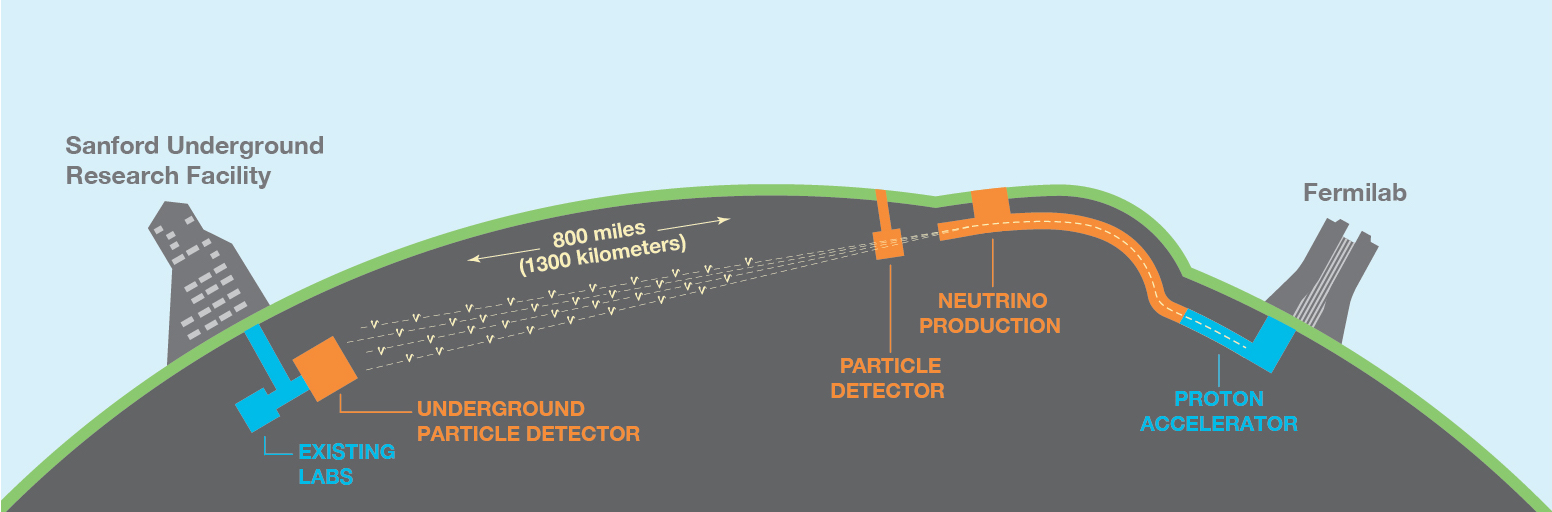
\includegraphics[width=0.99\textwidth]{figures/ch3-DUNE/LBNE_Graphic_061615_2016.jpg}
     \caption{Schematic representation of the DUNE experiment with its main components}
        \label{fig:DUNEdiagram}
\end{figure}
The Deep Underground Neutrino Experiment (DUNE) will be a next generation long baseline neutrino oscillation experiment \cite{DUNE:2020TDR1}. Its main goal will be to measure all the parameters governing neutrino and anti-neutrino oscillations in a single experiment, with particular emphasis on the CP violation phase $\delta_\textrm{CP}$ and the neutrino mass ordering. The experiment will consist of three main components: a wide band high intensity neutrino beam situated at Fermilab, which will be capable of producing both a $\nu_\mu$ and a $\Bar{\nu}_\mu$ fluxes; a kt-scale underground liquid Argon based Far Detector (FD), situated at the Sanford Underground Research Facility (SURF) in South Dakota, at $\sim1300$ Km from the source; a modular Near Detector (ND) situated at $\sim500$ m from the source.

Due to budgetary restrictions DUNE will pursue a staged approach in its construction and data production \cite{DUNE:2022Snowmass}. The initial composition of the experiment, referred to as Phase I, will include two LArTPC Far Detector modules, both being 10kt in volume, but utilizing a Vertical Drift \cite{DUNE:2023TDRVD} and an Horizontal Drift (or Single Phase) technology \cite{DUNE:2020TDR4} respectively. The initial configuration of the ND will include two out of the three originally envisioned detectors: the liquid argon near detector ND-LAr, a modular LArTPC similar in technology to the FD modules and the system for on axis neutrino detection SAND, whose main function will be to act as a beam monitor \cite{Battisti:2022ND}. A third ND module will be placed between ND-LAr and SAND to act as a muon spectrometer: this will be called the Temporary Muon Spectrometer (TMS) and will be removed from the ND facilities after Phase I to be replaced by a more capable detector. In Phase I DUNE will be able to determine the neutrino mass ordering, measure $\delta_\textrm{CP}$ at 3$\sigma$ if maximal, measure several oscillation parameters at world-leading levels of precision, detect supernova collapse neutrinos if available and search for BSM physics. 

In order to pursue its full physics scope, after Phase I DUNE will undertake several key improvements to all of its key components: this second form of the experiment is referred to as Phase II. The Far Detector will be completed by two extra liquid argon modules (nominally using the Verdical Drift technology) for a total fiducial mass of at least 40kt. The proton beam's power will augmented from 1.2 MW to 2.4 MW. The TMS will be replaced by a more capable high pressure gaseous Argon magnetized detector called ND-GAr. All of these upgrades are necessary for DUNE to reach one of its key stated goals: reach 5$\sigma$ sensitivity on CP violation over a wide range of $\delta_\textrm{CP}$ values. Additionally in Phase II, DUNE will be capable of producing independent measurements of $\sin^2{\theta_{13}}$ with precision comparable to that of reactors, it will have significant sensitivity to the $\theta_{23}$ octant, and will reach a world-leading sensitivity in a wide range of physics beyond the three neutrino paradigm as well as additional BSM physics and astrophysics. 

\section{DUNE's facilities and design}
In this section we give a brief overview of the components constituting the DUNE experiment, including the neutrino beamline, the Near Detector and the Far Detector. The muon spectrometer component of the Near Detector, which includes the ND-GAr detector for Phase I and the temporary muon spectrometer for Phase II, will be discussed in more detail in dedicated sections as they constitute the main focus of this thesis.


\subsection{The LBNF beamline}
\begin{figure}[!h]
     \centering
     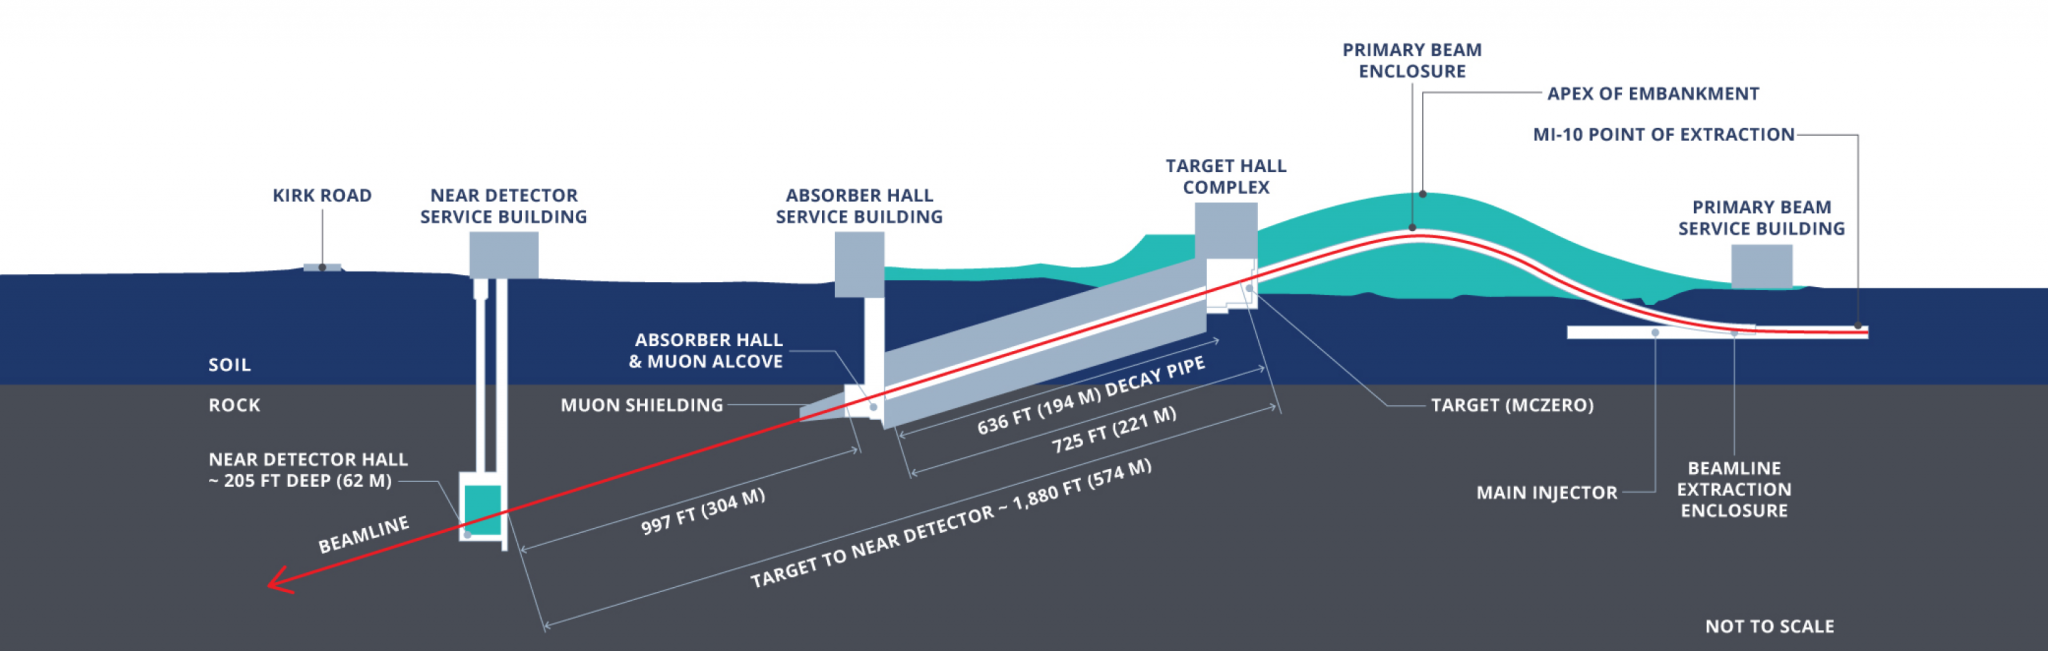
\includegraphics[width=0.99\textwidth]{figures/ch3-DUNE/LBNF-IL-graphic-Fermilab-LBNF.png}
     \caption{Schematic representation of the DUNE experiment with its main components}
        \label{fig:KFdiagram}
\end{figure}
The neutrino flux that will be utilized by the DUNE experiment, will be produced by the LBNF Beamline at Fermilab, which is expected to produce the highest power neutrino beam in the world \cite{DUNE:2016LBNFTDR, Papadimitriou:2016ksv}. The production of the neutrino flux begins by accelerating protons through a proton accelerator. The primary proton beam, which operates in the energy range of 60-120 GeV, is extracted from Fermilab's Main Injector (MI), a proton accelerator already utilized by the NOvA experiment and partially based on the Tevatron collider facilities. The main injector will be upgraded through the Proton Improvement Plan, phase II (PIP-II), in time for the DUNE Phase I data taking period to reach average beam powers of the order of 1.14 MW, delivering $7.5 \times 10^{13}$ protons in one MI machine cycle (0.7 sec - 1.2 sec) to the LBNF target. Further improvements are expected the PIP III project to reach 2.4 MW of power for DUNE Phase II and all the beamline components are being planned to accommodate these improvements with minimal retro-fitting. 

Once the primary proton beam reaches the desired energy, it is directed through the use of extraction and transport components over a man-made hill and bent downwards towards a graphite target located at grade level. This constitutes the first element of the proper neutrino beamline. The charged mesons, primarily kaons and pions, produced in the interactions of the protons are sign selected and focused by two magnetic horns into a decay pipe toward the far detector. The target and focusing horns are all located inside a heavily shielded vault called the target chase, that is isolated from the decay pipe at its downstream end by a metallic window. Their design is derived from that of the NuMi neutrino beam. 

The mesons produced in the proton interactions are short-lived and decay into either anti-muons and neutrinos or muons and anti-neutrino,s depending on the charge of the mesons. If the main neutrino types being produced are $\nu_\mu$ the Beamline is said to be in Forward Horn Current (FHC) mode, otherwise it is said to be in Reverse Horn Current (RHC) mode.  Both polarities will produced high purity
fluxes, with an expected contamination from the “incorrect” neutrino type (i.e. $\nu_\mu$ in RHC mode and vice-versa) of less than 10\% in the oscillation energy region. This type of impurities are introduced by hadrons of the opposite sign propagating at the centre of the beam, where no magnetic field is present. A small $\nu_e$ and $\Bar{\nu}_e$
component is also introduced by the decay of secondary kaons and tertiary muons from pion decays. At the end of the decay region, an absorber is needed to remove the residual hadrons remaining at the end of the decay pipe.  The absorber core consists of replaceable aluminium and steel water-cooled blocks. Approximately 40\% of the beam power is deposited in the target chase and surrounding shielding, 30\% in the decay pipe and 30\% in the absorber.

The wide band neutrino beam which is produced by the Beamline facilities, is needed to cover the first and second neutrino oscillation maxima, which for a 1300 km baseline are expected to be approximately at 2.4 and 0.8 GeV. For this reason the beamline design is optimized for neutrino energies between 0.5 and 5 GeV. 

\subsection{The Far Detector}
\begin{figure}[!ht]
     \centering
     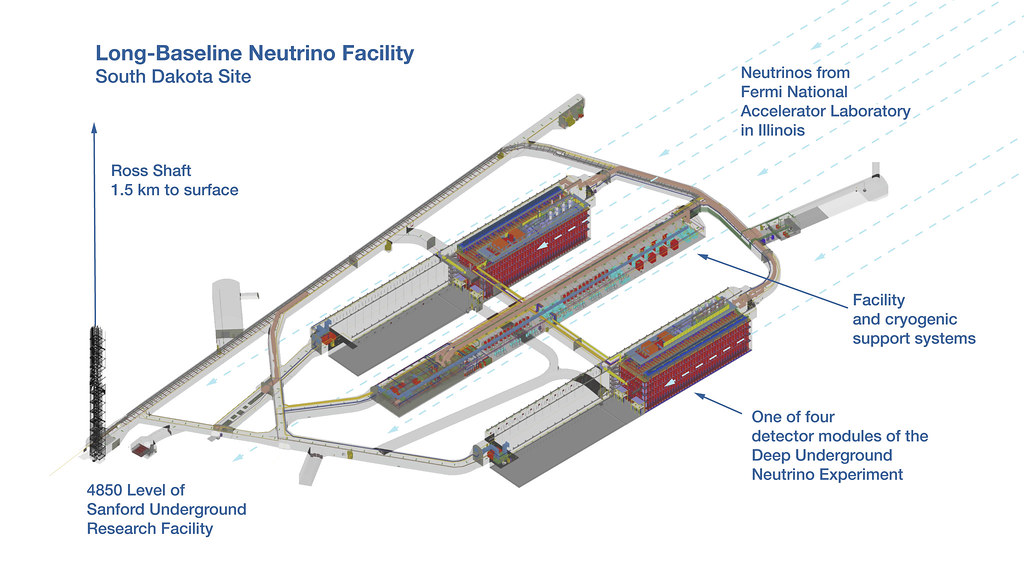
\includegraphics[width=0.99\textwidth]{figures/ch3-DUNE/Far_Detector.jpg}
     \caption{Schematic representation of the Far Detector experiment with its main components}
        \label{fig:DUNEdiagram}
\end{figure}
The DUNE Far Detector will be composed of four LArTPC detector module, each containing a 10kt fiducial liquid Argon mass  and a total liquid Argon mass of 17.5kt. Each module will fit inside a cryostat. Of the four modules only the first two will be available during DUNE Phase I, the first one using an Horizontal Drift technology (originally identified as Single Phase \cite{DUNE:2020TDR4}) will be called FD1-HD and the second one using a Vertical Drift technology\cite{DUNE:2023TDRVD} (evolved from the Dual Phase Technology \cite{DUNE:2018mlo}) will be called FD2-VD. The last two modules will be employed during Phase II and are nominally set to be Vertical Drift detectors\cite{DUNE:2022Snowmass}.

The LArTPC was pioneered by the ICARUS experiment \cite{Rubbia:1977zz,ICARUS:2004wqc} and is now a mature detector technology within the neutrino experiment community, being employed in detectors such as MicroBooNe\cite{MicroBooNE:2016pwy} and SBND\cite{Machado:2019oxb} at Fermilab as well as the ProtoDUNE-SP\cite{DUNE:2020cqd} prototype tested at the CERN neutrino facilities. In a LArTPC, ionization electrons produced by the energy deposition of charged particles generated in neutrino interactions, are drifted by an electric field in the liquid Argon towards an anode and are collected on a charge multiplier element, producing a readable two dimensional signal. The measurement of the collected ionization electrons also provides a measurement of the $dE/dx$ of the charged particles, which is what enables both calorimetry and particle identification (PID) in a LArTPC.

Argon is a UV light scintillator. Once shifted into the visible spectrum, the UV scintillation photons produced by can be collected by photon detectors and provide an initial start time $t_0$, indicating when the ionization electrons begin to drift. Comparing the time at which the ionization signal reaches the anode relative to this start time allows reconstruction of the event topology in the drift coordinate. 

The FD1-HD design combines a kt level fiducial mass with a sub-cm spacial resolution. Both are crucial to achieve DUNE's scientific goals of measuring CP violation, while searching for nucleon decay and being capable of observing neutrinos from supernova bursts. An example of the design of the detector being directly informed by the physics requirements of the experiment, comes from the electron/photon separation requirements necessary to study $\nu_e$ appearance signals in the LBNF $\nu_\mu$ flux. Electrons are typically produced in charged current $\nu_e$ interactions and induce electro-magnetic showers in the LAr medium. Similar electro-magnetic activity can be induced by photons coming for example from $\pi^0$ decay. The FD modules are capable of distinguishing between these two signals by using $dE/dx$ information combined with spacial information. Photon induced signals have an initial non ionized gap of several cm's before the formation of the electro-magnetic shower and have a $dE/dx$ which is double that of an electron induced one.

\begin{figure}[!t]
     \centering
     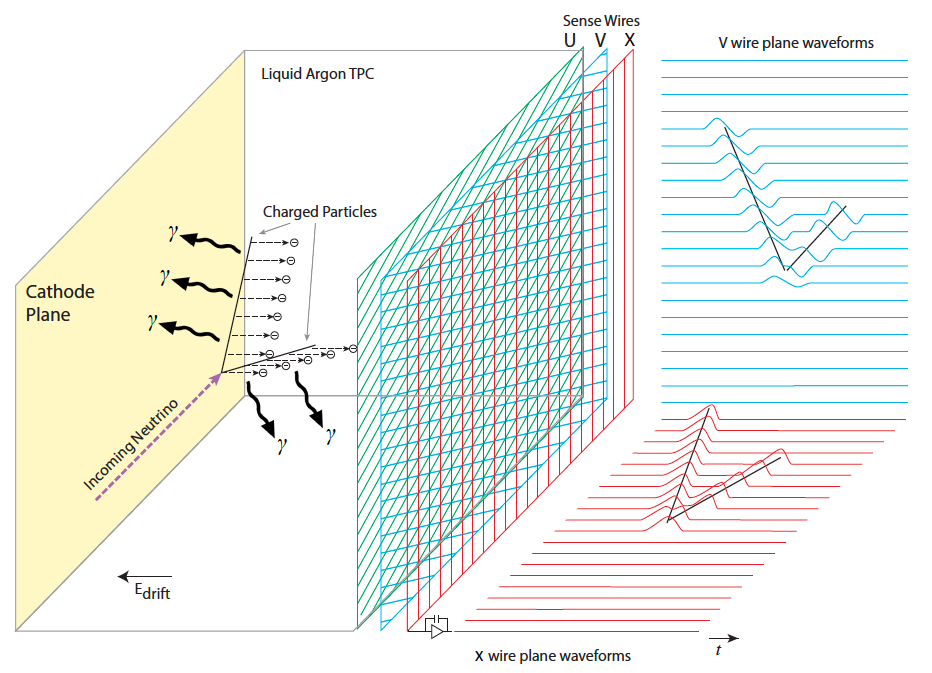
\includegraphics[width=0.8\textwidth]{figures/ch3-DUNE/TheBoPicture.png}
     \caption{Schematic representation of the Far Detector experiment with its main components}
        \label{fig:DUNEdiagram}
\end{figure}

The FD1-HD detector modules consist of 4 separate liquid Argon filled drift volumes with a maximum drift length of 3.5 m. Each Volume is instrumented with a vertical cathode plane and an anode plane, for a total of three module-long (58.2 m) anode planes and two cathode planes. A field cage covers the spaces between the two, producing a stable 500 V/m electric field in the horizontal direction. The drift ionization electrons reach the anode planes in an order of a few milli-seconds. 

Each anode plane is instrumented with a total of 50 anode plane assemblies APAs which consist of an aluminum frame with three layers of active wires and an additional shielding layer wrapped around them. The first two active layers are identified as the U and V induction layers. These layers are angled at a $\pm 37.5^\circ$ in order to reduce ambiguities in event reconstruction. The relative voltage between the layers is chosen so that the drift electrons pass through them and produce a bipolar induction signal on both planes. The drifting electrons are finally collected in the final $X$ wire plane, where they produce a mono-polar signal. In the $X$ collection plane, as well as in the $G$ shielding plane, the wires run vertically. The spacing between the wires in each layer is of 5 mm, and defines the spacial resolution of the APAs.

The scintillation photons produced by the passing charged particles in the liquid Argon in the very ultra violet (VUV) spectrum are collected by photon detector (PD) systems called X-ARAPUCA \cite{Segreto:2018jdx}. The photons are produce in the order of 24000 per MeV of deposited energy, and reach the detectors in a time-frame of the order of a nanosecond. The X-ARAPUCA modules are mounted between the sets of wire-planes and consist of layers of dichroic filter and wavelength shifters, that shift the VUV scintillation light into the visible range, trap the visible photons, and transport them to a silicon photo-multiplier (SiPM). The signals produced in the SiPMs are then combined with the wire signals from the APAs at the data acquisition (DAQ) level.

\begin{figure}[!t]
     \centering
     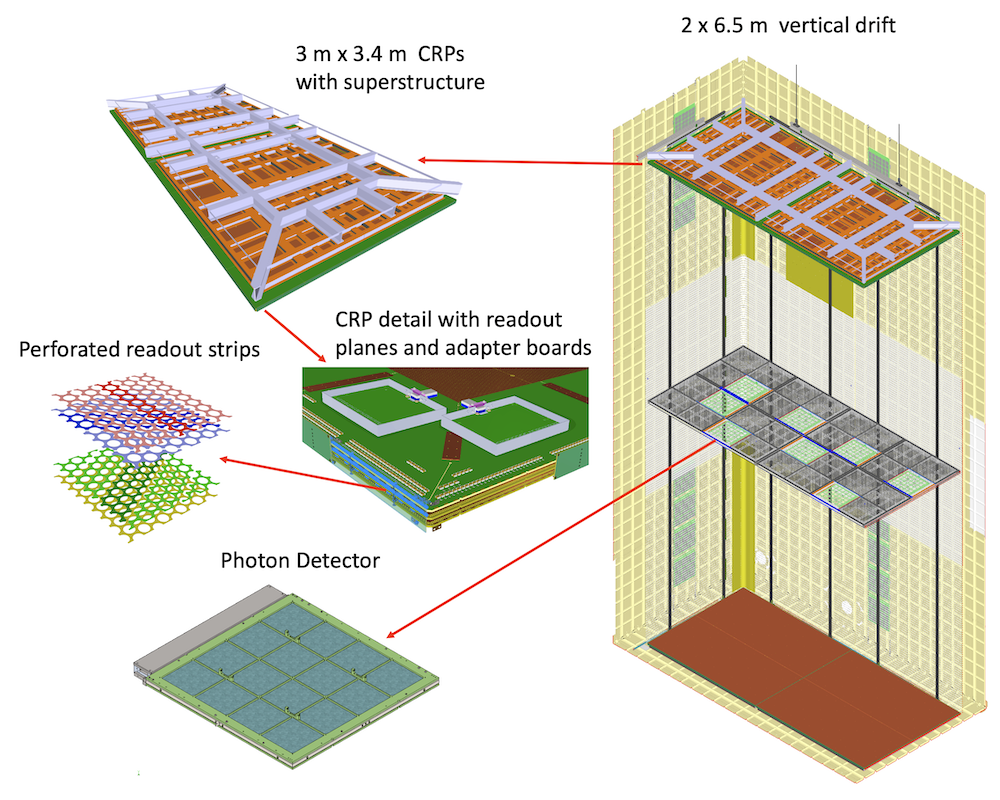
\includegraphics[width=0.7\textwidth]{figures/ch3-DUNE/setup_new_updated.png}
     \caption{Schematic representation of the Far Detector experiment with its main components}
        \label{fig:DUNEdiagram}
\end{figure}

The FD2-VD design has developed from the R\&D experience accumulated by the DUNE collaboration with the ProtoDUNE-SP and ProtoDUNE-DP prototypes at the neutrino research facilities at CERN. The detector consists of several vertical drift modules enclosed in a large cryostat structure. Each module is divided into two vertical drift regions 6.5 m in height, by an horizontal cathode and feature two anode planes, one close to the cryostat top, just below the surface of the liquid Argon region and one close to the bottom of the cryostat. Field cage modules hang vertically around the module's perimeter. The 450 V/cm electric field drifts the ionisation electrons, either upwards or downwards depending on the drift region. The vertical design of the FD2-VD offers a slightly larger instrumented module compared to FD1-HD and it's more cost-effective thanks to its high-modularity and general structure and geometry. 

The anode planes in the FD2-VD design consist of two double-sided perforated printed circuit boards (PCBs) that are connected to form a charge-readout unit (CRUs). The perforation holes allow the electrons to pass through the PCB's. The first PCB is instrumented with two sets of induction strips, while the second one hosts the collection strips. The three planes of strips are segmented at about 7.5 mm pitch for the induction planes and 5 mm pitch for the collection plane, and are set at $60^\circ$ angles relative to each other to maximize information in the charge readout from different projections. Two CRU's are connected to a frame to form a Charge Readout Plane (CRP). Each anode plane consists of 80 CRP's. Much like in the FD1-HD design the anode plane signal allows for a two-dimensional reconstruction of any given event, while the third dimension is given by the drift time information obtained from the scintillation light.

The PD's implemented in the FD2-VD follow the same general design of the ARAPUCA-X modules developed for FD1-HD. The PDs will be mounted on the four cryostat membrane walls as on both sides of the central cathode structure. This configuration offers a uniform ligth measurement coverage across the entire LArTPC volume. Additionally, the FD2-VD liquid argon will be doped with a small quantity of xenon. This has no impact on the TPC operation but significantly enhances the photon detection performance.

\subsection{The Near Detector}

\begin{figure}[!h]
     \centering
     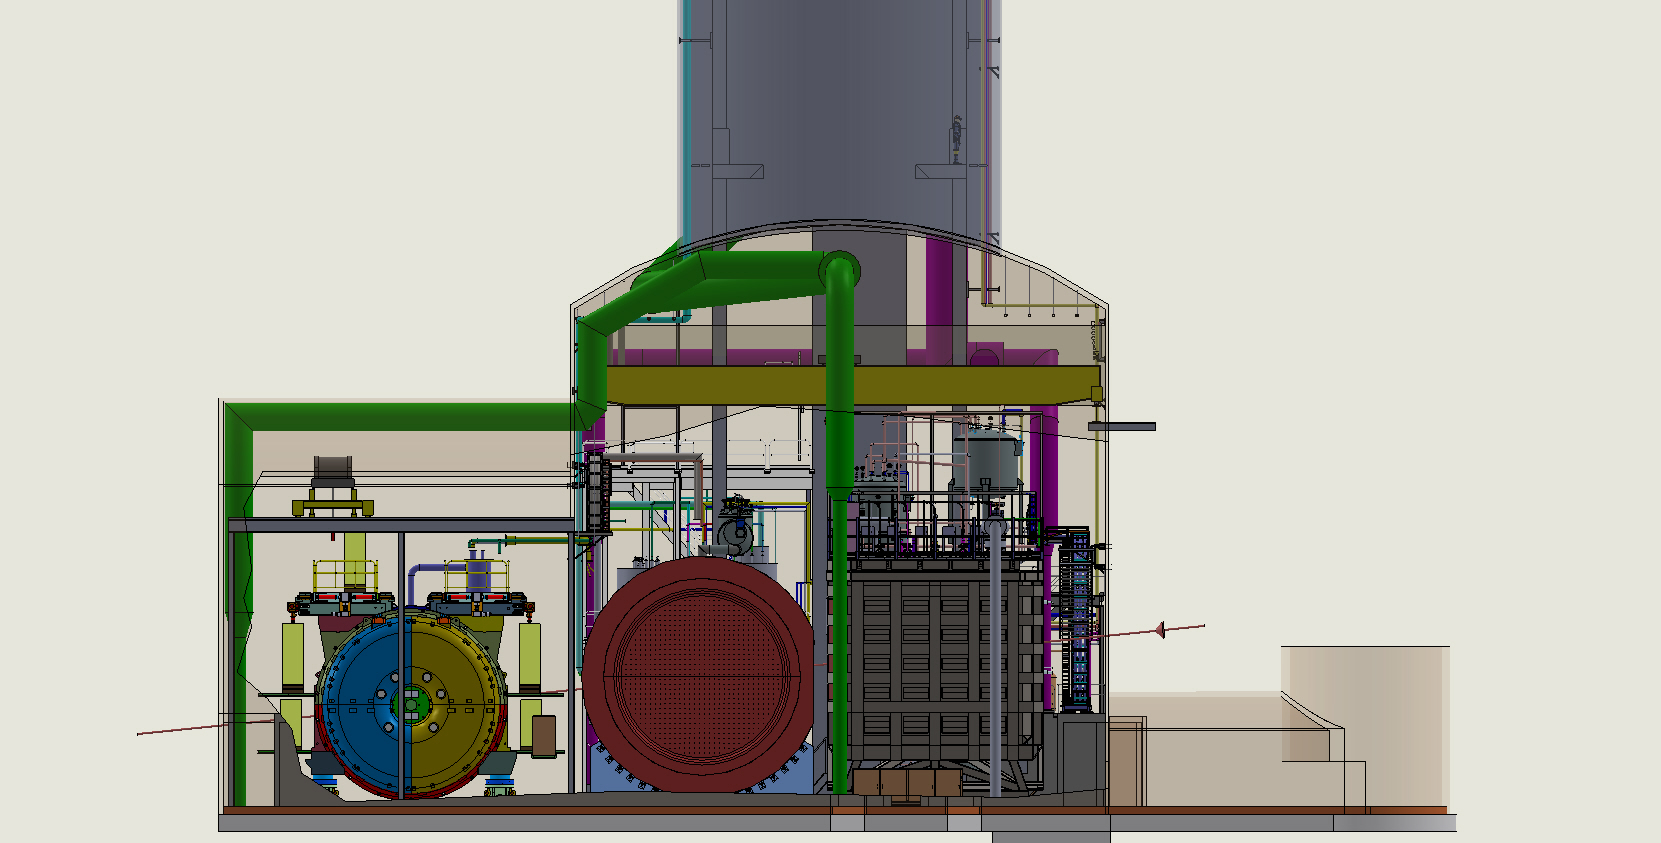
\includegraphics[width=0.99\textwidth]{figures/ch3-DUNE/ndhall.JPG}
     \caption{Schematic representation of the Far Detector experiment with its main components}
        \label{fig:NDhall}
\end{figure}

To enable oscillation measurements, DUNE must first predict the anticipated signal and background at the Far Detector based on oscillation parameters, followed by a comparison with measured flavour-tagged neutrino spectra. To generate this prediction, one must determine the neutrino flux at production, neutrino interaction cross-sections, and detector response—factors all affected by systematic uncertainties requiring constraint. The Near Detector (ND) is tailored to address each prediction component \cite{DUNE:2021NDCDR}: it will gauge the un-oscillated neutrino beam flux both on-axis and at varying off-axis angles; refine models of neutrino interactions through cross-section and final state topology measurements; model detector responses relative to neutrino energy. Additionally, the ND is designed for operation within a high event rate environment, ensuring the requisite statistical coverage across the full phase-space. The ND will be of three detectors with complementary designs: ND-LAr, which will use a LArTPC technology similar to the FD modules; ND-GAr, a gaseous Argon TPC detector; and SAND, a magnetized beam monitor. ND-LAr and ND-GAr are movable off-axis and will contribute to the DUNE-PRISM program, while SAND remains fixed on-axis. A schematic depiction of the Near Detector, inclusive of all detectors, is presented in Figure \ref{fig:NDhall}. Due to budgetary reasons the ND-GAr detector will become available only during Phase II of the DUNE experiment. A much simpler detector referred to as the Temporary Muon Spectrometer (TMS) will replace it during Phase I. Both ND-GAr and the TMS will be discussed in a dedicated section along-side an alternative and now abandoned Phase I muon spectrometer design called ND-GAr-Lite. 


\begin{figure}[!t]
     \centering
     \begin{subfigure}[b]{0.59\textwidth}
         \centering
         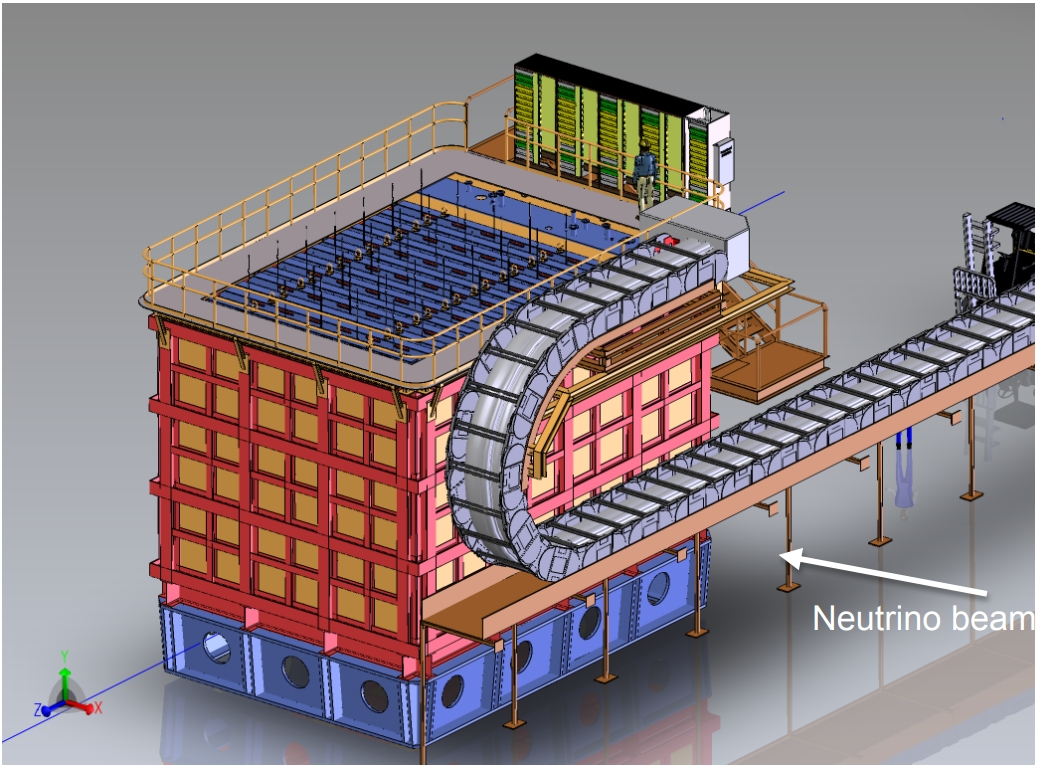
\includegraphics[width=\textwidth]{figures/ch3-DUNE/ND-LAr.jpg}
         \caption{}
         \label{fig:NDLAr}
     \end{subfigure}
     \begin{subfigure}[b]{0.39\textwidth}
         \centering
         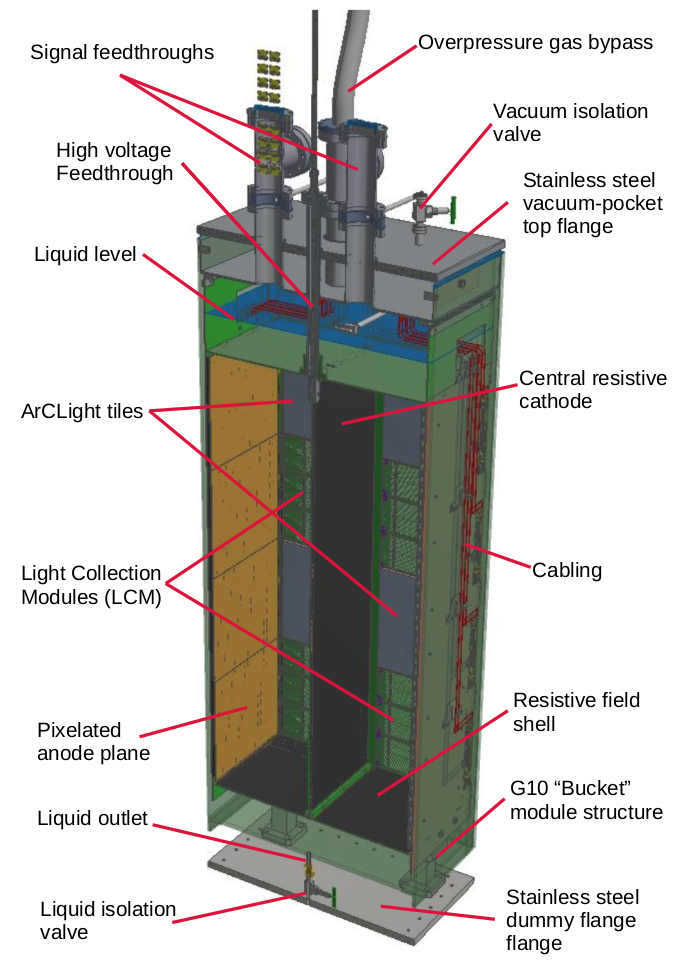
\includegraphics[width=\textwidth]{figures/ch3-DUNE/ND-LAr_module.png}
         \caption{}
         \label{fig:NDLArModule}
     \end{subfigure}
        \caption{(a) Average $\beta$ as a function of the track length $l $ and  (b) average track length as a function of the true momentum $p_\textrm{true}$ for the HP sample.}
        \label{fig:ND-Larview}
\end{figure}

ND-LAr is a LArTPC detector engineered for operation within a high-rate environment. Utilizing the same Argon target and similar detector technology as the FD modules, ND-LAr is essential for modeling detector response and liquid Argon neutrino interaction cross-sections. ND-LAr is comprised of 35 distinct TPC modules, mirroring the design of the ArgonCube prototype \cite{Dwyer:2018phu}. Despite the relativly modest dimentions of the detector, this modular architecture is indispensable for managing the high event rate, facilitating a smaller drift region, enhanced light separation, and increased sensor pixelation. Each module encompasses two optically isolated TPCs outfitted with a LArPix-based pixelated charge readout system  \cite{Goldi:2018mbo}, alongside a light readout for rapid timing data from prompt scintillation light, and a field structure ensuring minimal field non-uniformity throughout the active volume. Given the relatively compact dimensions of its active volume, ND-LAr cannot fully contain the majority of muons generated in $\nu_\mu$ Charged Current (CC) interactions within liquid Argon. Hence, precise momentum reconstruction of this muon sample necessitates an external spectrometer component, a role fulfilled by ND-GAr and the TMS.

\begin{figure}[t]
     \centering
     \begin{subfigure}[b]{0.5\textwidth}
         \centering
         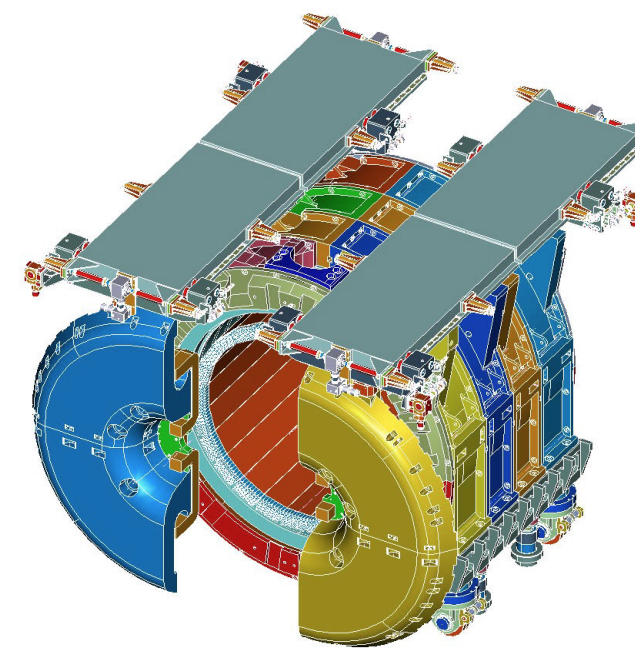
\includegraphics[width=\textwidth]{figures/ch3-DUNE/SAND.png}
         \caption{}
         \label{fig:SAND-outside}
     \end{subfigure}
     \hfill
     \begin{subfigure}[b]{0.48\textwidth}
         \centering
         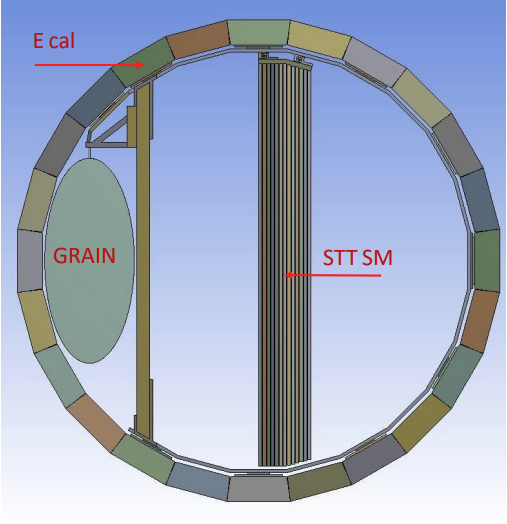
\includegraphics[width=\textwidth]{figures/ch3-DUNE/SAND-inside.png}
         \caption{}
         \label{fig:SAND-inside}
     \end{subfigure}
        \caption{(a) Schematic view of the external components of SAND, including its cryostat and its solenoid magnet (b) Side view of the internal components of SAND, including its active liquid Argon target called GRAIN, one of the straw tube tracker modules and the electro-magnetic calorimeter.  }
        \label{fig:SAND-all}
\end{figure}

ND-LAr and ND-GAr possess the capability to be translated up to 30 meters perpendicular to the neutrino beam axis, spanning angles from $0^{\circ}$ to $3^{\circ}$, a feature named DUNE-PRISM. With increasing off-axis angles, the mean energy of the neutrino flux diminishes while its energy dispersion narrows. Consequently, the Near Detector gains access to diverse un-oscillated neutrino flux profiles, combining them to predict the oscillated flux at the far detector. This data-centric methodology mitigates reliance on models. Moreover, a key feature of the DUNE-PRISM program is that the off-axis fluxes will variate in mean energies and spreads and will thus be dominated by distinct interaction types (e.g., quasi-elastic, resonant etc.). Access to this variety of samples will facilitate the disentanglement of cross-section effects, enhancing flux and interaction modeling.

The System for On-Axis Neutrino Detection (SAND) will function as a constant on-axis monitor of the neutrino beam, a crucial role for the DUNE-PRISM program. It will ensure that any differences in flux measured by ND-LAr and ND-GAr result from their off-axis position rather than anomalies in beam production. SAND's main structural components, along with its solenoid magnet, cryostat, and electromagnetic calorimeter, will be repurposed from the KLOE experiment (Figure \ref{fig:SAND-all}). The internal tracker design of SAND has recently been finalized, featuring a Straw Tube Tracker (STT) divided in modules. These modules will include a series of tunable passive slabs interleaved with tracking layers of 5mm diameter tubes. SAND will provide various targets, such as CH$_2$ and C, potentially highly useful in studying neutrino interactions. They will offer a clean sample of neutrino-on-hydrogen interactions by "subtraction," devoid of nuclear effects. Additionally, SAND will incorporate its own active target of liquid Argon called GRAIN, whose design is currently being finalized. 

\section{The ND-GAr detector}
% \begin{figure}
%      \centering
%      \begin{subfigure}[b]{0.4\textwidth}
%          \centering
%          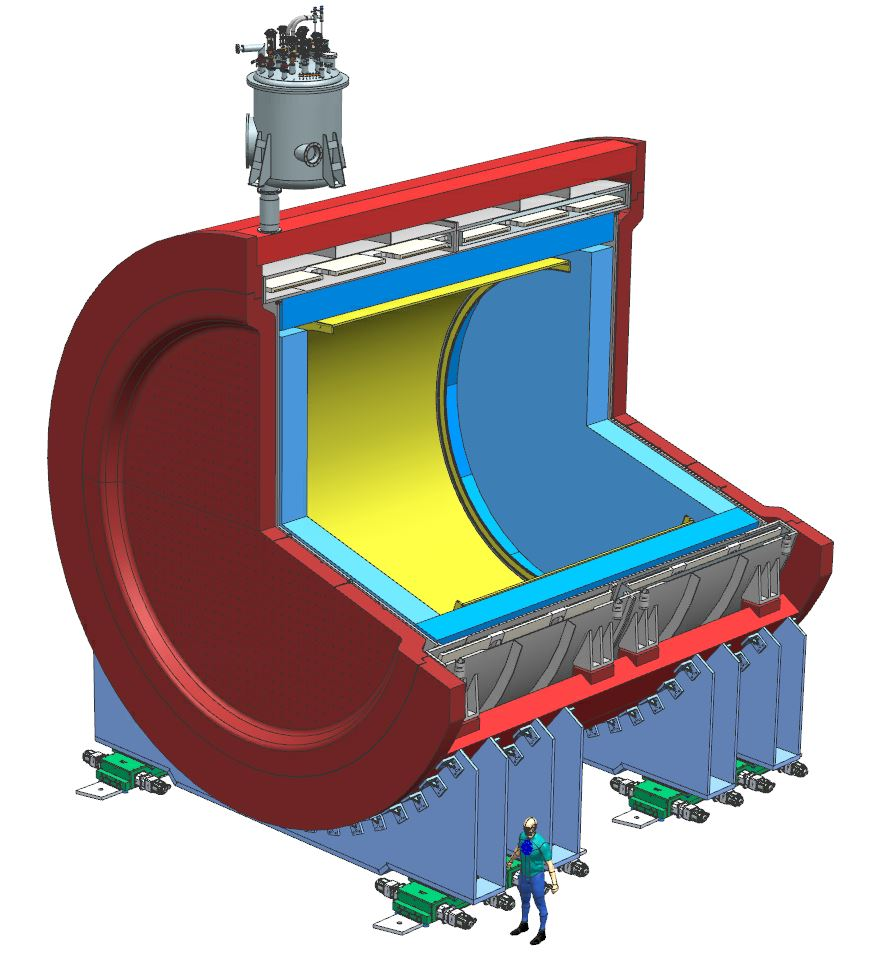
\includegraphics[width=\textwidth]{figures/ch3-DUNE/ND_GAr.jpg}
%          \caption{}
%          \label{fig:ND-G}
%      \end{subfigure}
%      \hfill
%      \begin{subfigure}[b]{0.58\textwidth}
%          \centering
%          \includegraphics[width=\textwidth]{figures/ch3-DUNE/SPY_X-section2.jpg}
%          \caption{}
%          \label{fig:ND-G-threshold}
%      \end{subfigure}
%         \caption{(a) Schematic view of the external components of ND-GAr with a cutaway showing the magnet, electro-magnetic calorimeter and the internal TPC  (b) Plot showing proton range in cm as a function of Kinetic Energy in MeV in double logarithmic scale. The different curves show the range dependency in different gaseous, liquid or solid media \cite{Lu}. }
%         \label{fig:GAr}
% \end{figure}

\begin{figure}[t]
     \centering
     \includegraphics[width=0.6\textwidth]{figures/ch3-DUNE/SPY_X-section2.jpg}
     \caption{Schematic representation of ND-GAr experiment with its main components}
        \label{fig:ND-G}
\end{figure}

ND-GAr will be a magnetized detector with a magnetic field of 0.5T, mainly constituted of a high pressure gas time projection chamber (HPgTPC) surrounded by an electro-magnetic calorimeter (ECAL). A simple cut-away schematic of the detector is shown in Figure \ref{fig:GAr}. ND-GAr will fulfill two main goals: firstly it will act as a spectrometer measuring the charge and momentum of particles exiting ND-LAr; secondly it will offer its own sample of neutrino interactions inside the HPgTPC. The high pressure gas environment will offer relatively low tracking thresholds and enhanced particle identification (PID) performance when compared to LArTPC's, especially for pion-proton separation. The PID capabilities of ND-GAr specifically derive from a combination of $dE/dx$ measurements in the HPgTPC, $E/p$ measurements in the ECAL and the curvature momentum and sign selection measurements available from the magnetization of the TPC alongside range measurements in the ECAL.

ND-GAr's spectrometer role mostly consists in identifying the sign and measuring the momentum of muons exciting ND-LAr. This is done to measure the spectrum of $\nu_\mu$ and $\Bar{\nu}_\mu$ reaching the near detector, through their CC interaction products. This is crucial to reach the oscillation measurement sensitivity desired by the experiment.

\begin{figure}[t]
     \centering
     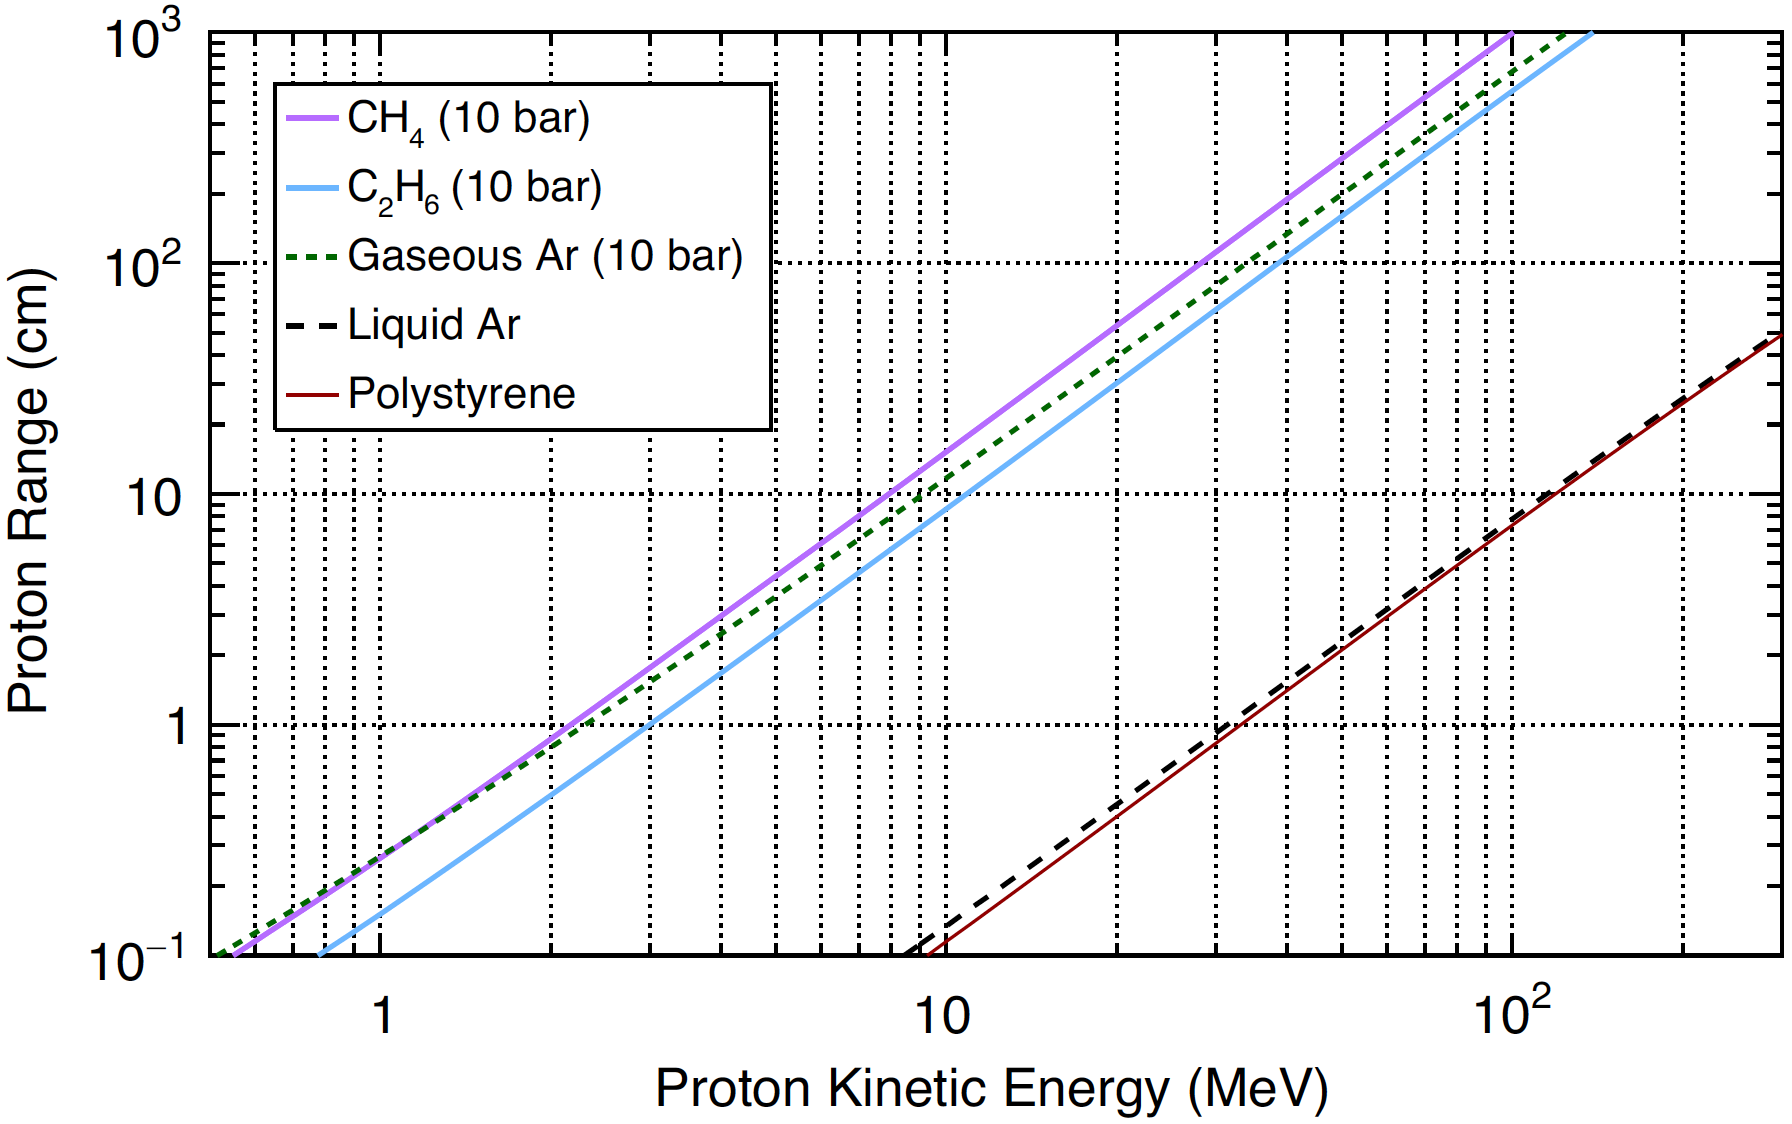
\includegraphics[width=0.7\textwidth]{figures/ch3-DUNE/threshold.png}
     \caption{Schematic representation of ND-GAr experiment with its main components}
        \label{fig:ND-G-threshold}
\end{figure}

ND-GAr's lower tracking thresholds as well as its superior PID capabilities and acceptance, will make kinematic regions not accessible to a LAr detector, available to the ND complex. The relationship between proton tracking threshold and tracking material can be seen in Figure \ref{fig:ND-G-threshold}. This is particularly important to enhance the ability of the ND of clarifying the relationship between the true and reconstructed energy in neutrino interactions on Argon. Nuclear effects such as final state interactions (FSI), Fermi motion and 2p2h effects can introduce significant systematic uncertainties in the reconstruction of the neutrino energy. Theoretical studies suggest for example that FSI can increase dramatically the number of final state protons in the kinetic range of 10s of MeV's and it's thus crutial for the ND to be able to measure them and identify them. This is possible with a HpGTPC which has lower tracking thresholds, but not in a LAr or solid detector such as ND-LAr or SAND. 

It is also important for ND-GAr to characterize the spectrum of charged pions coming from $\nu_\mu$ and $\Bar{\nu}_\mu$ CC interactions. At very low energies, down to 20 MeV , this is essential because this is the region where FSI's are more prevalent. Only a gaseous detector has low enough energy thresholds to do it with a sufficient efficiency. At higher energies above 100 MeV, ND-GAr becomes essential in distinguishing the pion multiplicity, since in LAr the same pions tend to produce hadronic showers, while in ND-Gar's TPC they are more likely to  produce distinguishable tracks. Measuring neutral pions from $\nu_\mu$ and $\Bar{\nu}_\mu$ CC interactions in the same momentum range is also possible for ND-GAr thanks to its ECAL.

\subsection{The HpGTPC}
The design of ND-GAr's HPgTPC is closely related to the design of the ALICE experiment's TPC \cite{ALICE}. The basic detection mechanisms of ALICE's and ND-GAr's TPC's are identical. The primary ionization electrons are formed by the energy deposition of passing charged particles, and drifted towards the end-caps by a an electric field produced by a high voltage (HV) central electrode plane. The total drift region has a cylindrical shape with a diameter of $\sim 5m$ and a length of $\sim 5m$ and the electric field is oriented in parallel to the 0.5T magnetic field, in order to reduce transverse diffusion. At the end-caps, multi-wire proportional chambers (MWPC's) induce electron avalanches which produce a signal on an anode pad plane. Read-outs of the pad signals give hit coordinates in two dimensions, while the drift time provides the third.

The read-out chambers or ROC's used in ALICE, contain the MWPC's and read-out pad planes and are divided in 18 trapezoidal regions, each including a smaller inner chamber (IROC) and an outer chamber (OROC). All of ALICE's ROC's will be re-installed in ND-GAr, as they have been replaced in the original detector by GEM-based ROC's \cite{Ferretti:2022yjd}. An additional central region of ROC's (CROC's) will fill the central regions of the read-out planes, which in ALICE was occupied by a silicon based central tracker and an inner field cage. 

Despite all the common elements, some key differences between the design of the two TPC's exist: the two detectors will use different gases, with ALICE's base gas being a mixture Ne/CO$_2$/N$_2$ and ND-GAr using a mixture of Ar-CH$_4$ at 90\%-10\% molar fractions; ND-GAr will operate at a pressure 10 times larger than ALICE; the electronics and data acquisition systems will be completely re-designed to be closer to the LArPix technologies used in DUNE's LArTPC's; the field cage will only include an outer component, since the central region in ND-GAr will be part of the active volume of the detector, while in ALICE it was occupied by the the beam pipe and a silicon-based tracker.
\begin{figure}[t]
     \centering
     \begin{subfigure}[b]{0.52\textwidth}
         \centering
         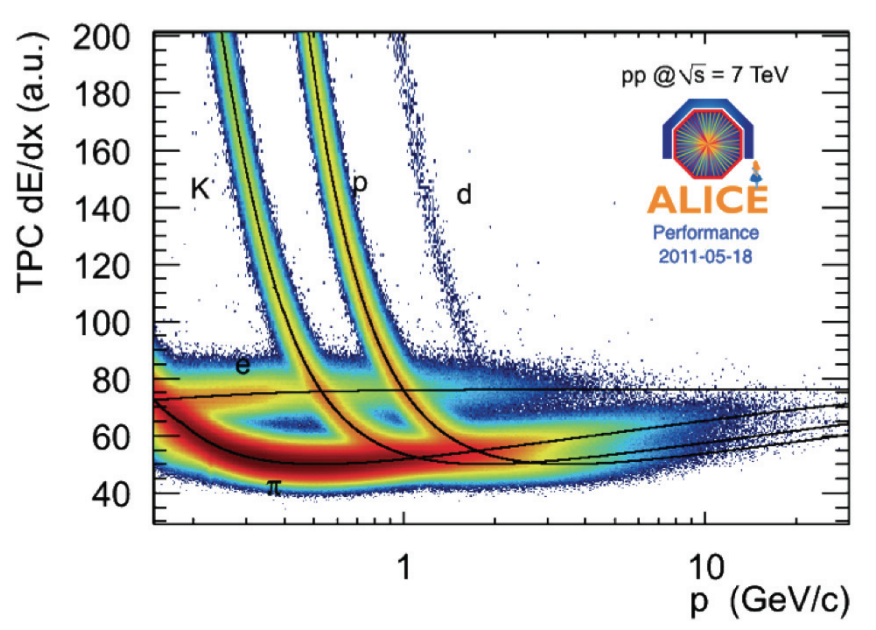
\includegraphics[width=\textwidth]{figures/ch3-DUNE/ALICE_TPC_dEdx_Lippmann_2012.png}
         \caption{}
         \label{fig:ALICEPID}
     \end{subfigure}
     \hfill
     \begin{subfigure}[b]{0.47\textwidth}
         \centering
         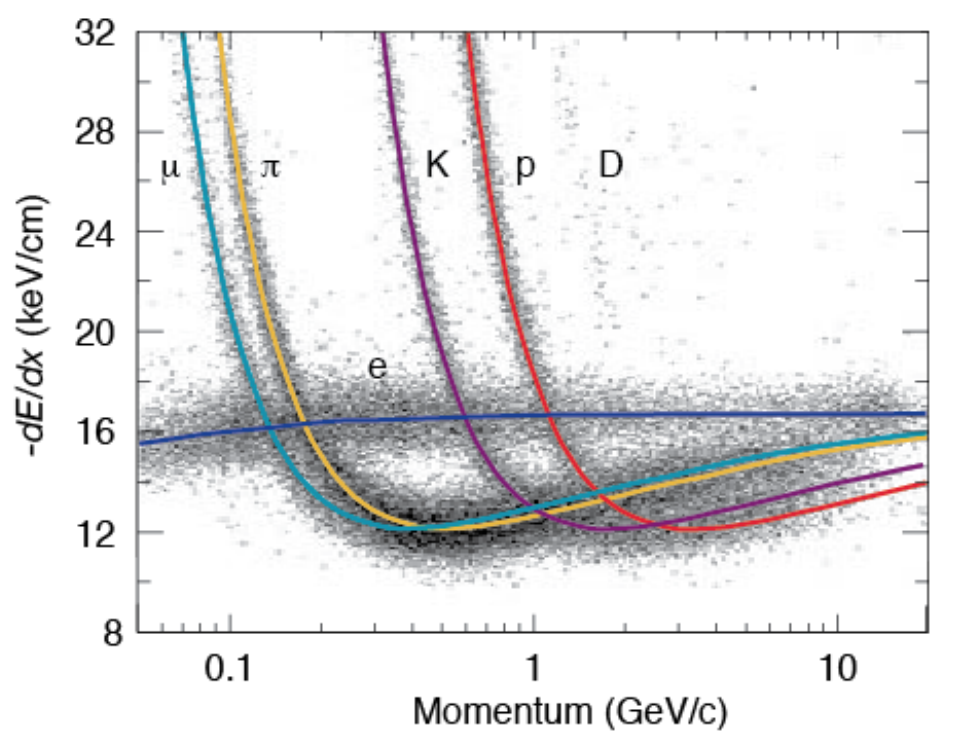
\includegraphics[width=\textwidth]{figures/ch3-DUNE/PEP4-TPC-80Ar-20CH4-8_5atm_dEdx.png}
         \caption{}
         \label{fig:PEPPID}
     \end{subfigure}
        \caption{(a) Schematic view of the external components of ND-GAr with a cutaway showing the magnet, electro-magnetic calorimeter and the internal TPC  (b) Plot showing proton range in cm as a function of Kinetic Energy in MeV in double logarithmic scale. The different curves show the range dependency in different gaseous, liquid or solid media \cite{Lu}. }
        \label{fig:PID}
\end{figure}

The HPgTPC is oriented so that the neutrino beam is perpendicular to the electric and magnetic fields. This is the most favorable orientation for measuring charged particles traveling along the neutrino beam direction. In ALICE the track reconstruction is done by combing ROC hits to form tracks following the trajectories of charged particles in the TPC. This is done for ND-GAr through the GArSoft software package which handles the simulation and reconstruction for the detector. A comprehensive description of this tool will be given later in Sec. and Sec. respectively. 

In ALICE the ionization induced by charged particle tracks can be used to estimate the particle's $dE/dx$. When combined with a curvature momentum estimate, this can be used for PID. In Fig. \ref{fig:ALICEPID} we show the characteristic PID curves for charged particles produced in proton-proton collisions at $\sqrt{s}=7 \textrm{TeV}$. The band resolution of the different particle types $dE/dx$ curves is expected to be significantly improved in ND-GAr. The 10 times higher gas pressure in ND-GAr will result in a correspondend increase in ionization per unit track length. A better comparison can thus be made with the performance of the PID capabilities of PEP-4/9, which operated at 8.5 atmospheres: the experiment's $dE/dx$ curves are plotted in Fig. \ref{fig:PEPPID} showing good separation between particle types below a few GeV, including pions and muons which are problematic for lower material budget TPC's. 

\begin{figure}[t]
     \centering
     \begin{subfigure}[b]{0.47\textwidth}
         \centering
         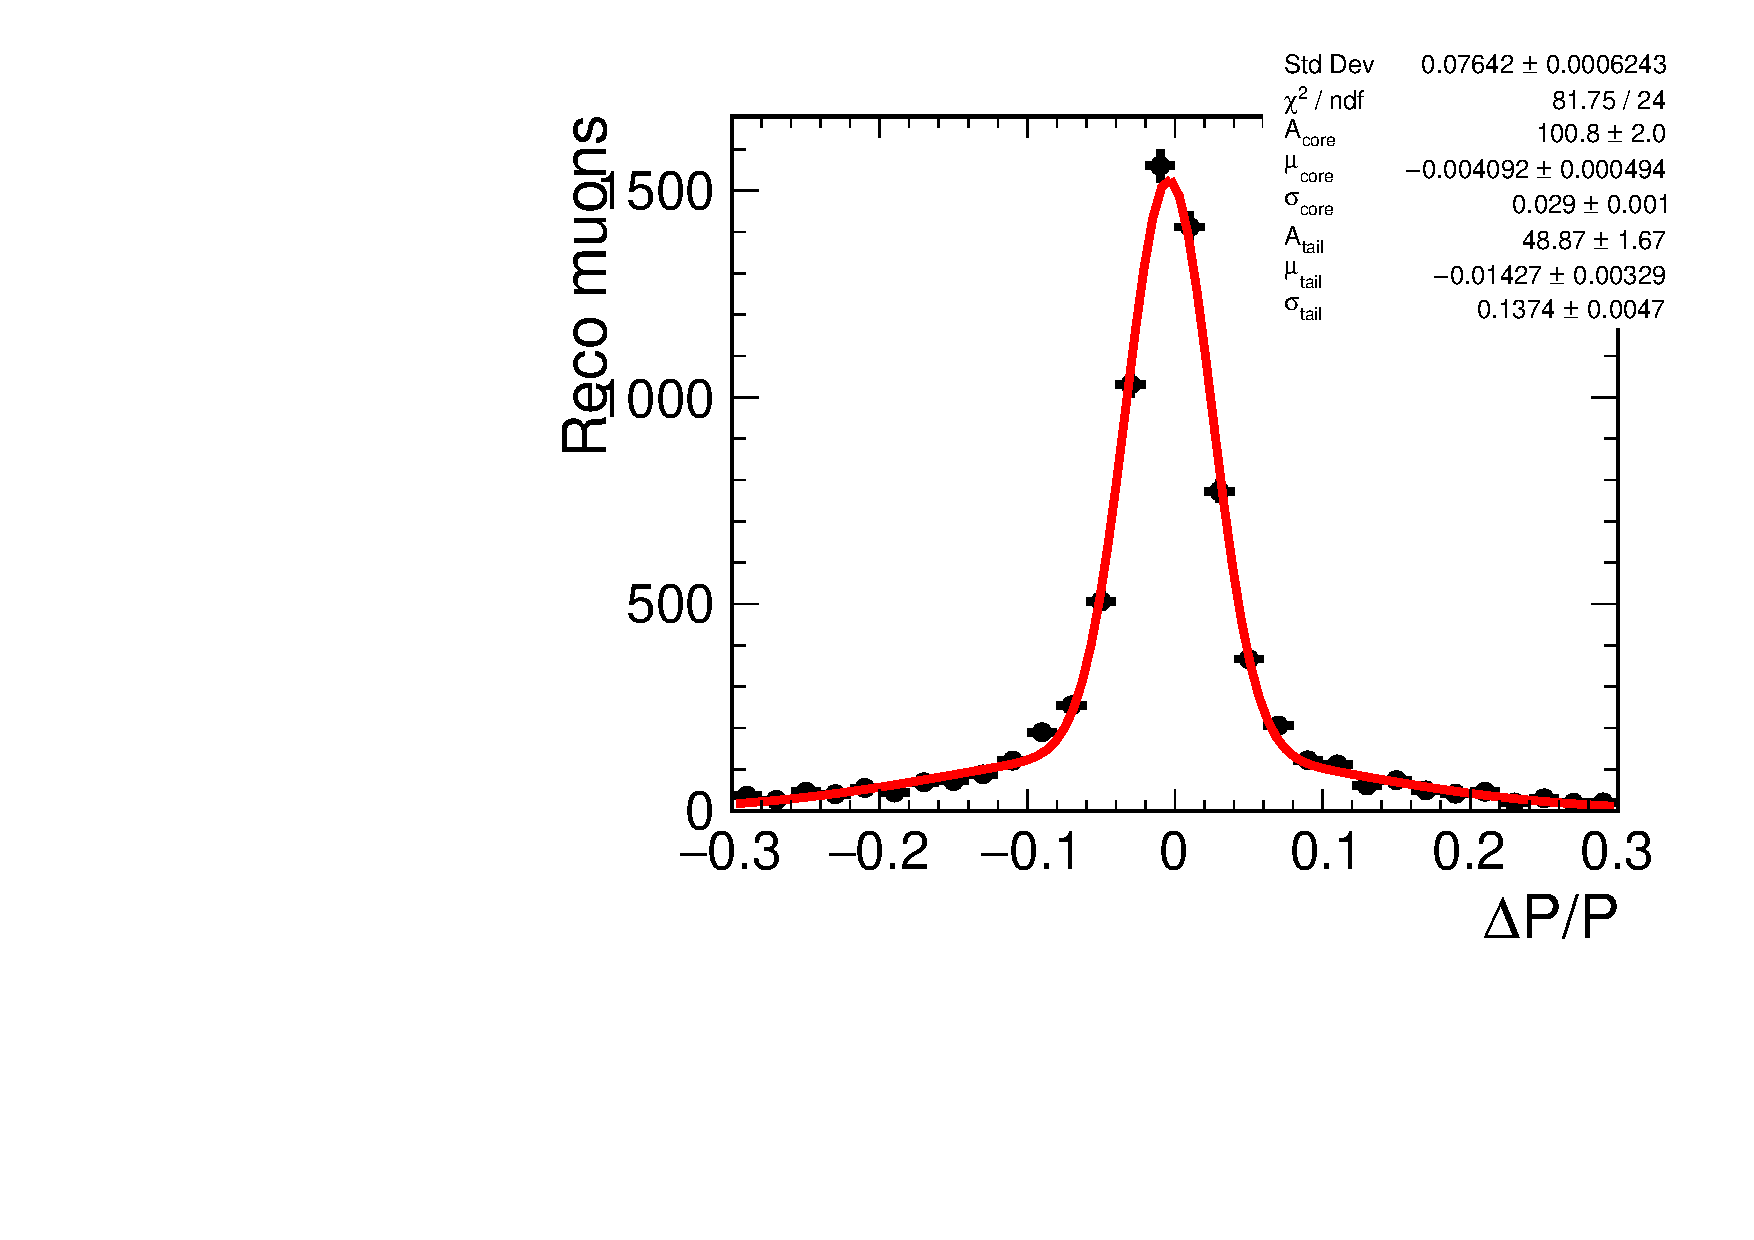
\includegraphics[width=\textwidth]{figures/ch3-DUNE/dpmuon.pdf}
         \caption{}
         \label{fig:GArTPCdp}
     \end{subfigure}
     \hfill
     \begin{subfigure}[b]{0.52\textwidth}
         \centering
         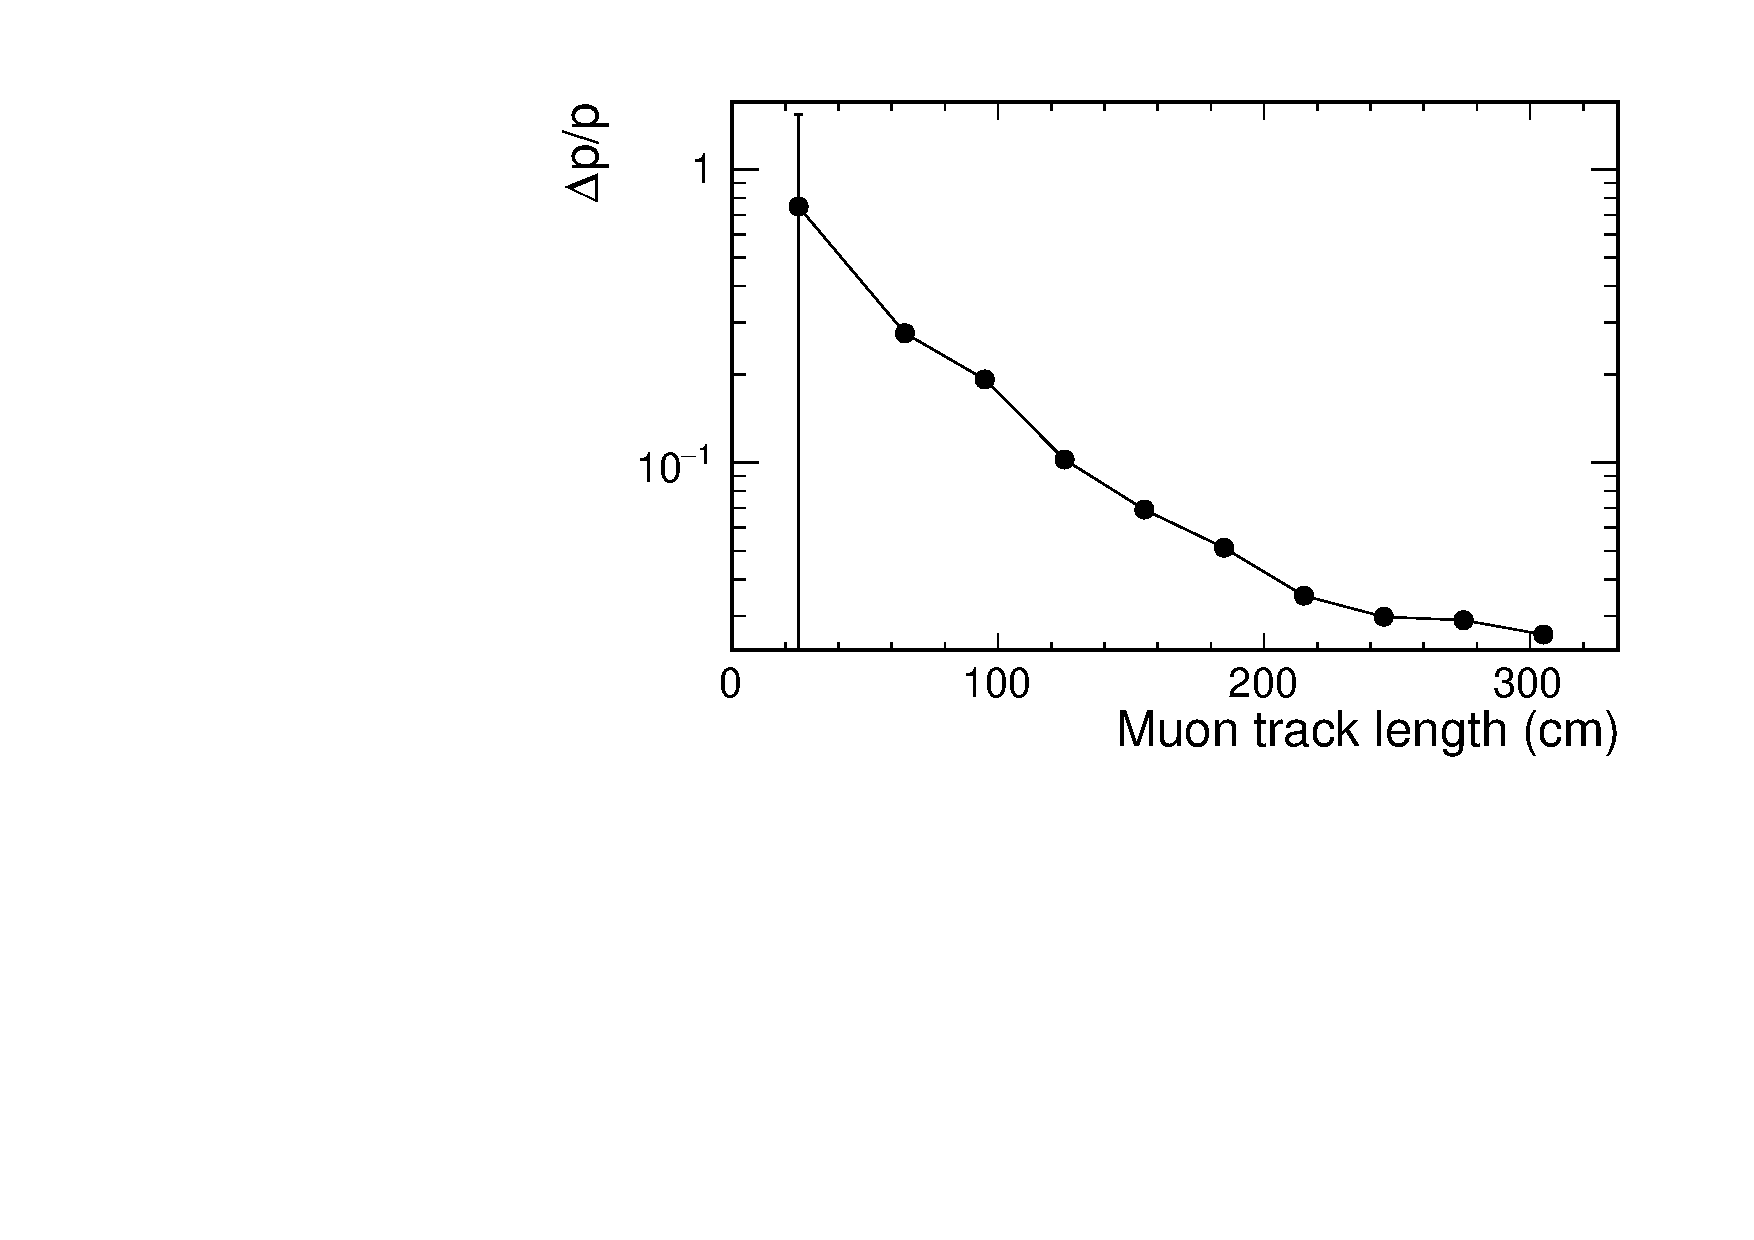
\includegraphics[width=\textwidth]{figures/ch3-DUNE/muonpoverpfunc.pdf}
         \caption{}
         \label{fig:GArTPCdpoverp}
     \end{subfigure}
        \caption{(a) Schematic view of the external components of ND-GAr with a cutaway showing the magnet, electro-magnetic calorimeter and the internal TPC  (b) Plot showing proton range in cm as a function of Kinetic Energy in MeV in double logarithmic scale. The different curves show the range dependency in different gaseous, liquid or solid media \cite{Lu}. }
        \label{fig:GARTPCdp}
\end{figure}

The resolution of a curvature momentum measurement in a TPC depends on the pad resolution as well as the multiple coulomb scattering (MS) degradation (see Sec for a more in depth discussion). The characteristics of the track and of the neutrino event also influence the curvature resolution. These include the particle's transverse momentum $p_T$ the track's length as well as the detector's occupancy at the time of the track formation.

Given the randomized nature of particle track formation in a neutrino experiment, the distribution of the tracks length is expected to have a significant component of short tracks. For this reason fiducial cuts are imposed inside the TPC. Note that low energy particles that stop within the detector (primarily protons) would be reconstructed via their track length rather than their curvature. Within the fiducial volume ND-GAr will have a $4\pi$ acceptance. This include particles crossing the central cathode region, which is very thin (25 $\mu m$ of mylar).

An early study was done using the GArSoft software suite, on the momentum resolution for muons coming from $\nu_\mu CC$ interactions in the HpGTPC using the LBNF flux. A fiducial cut was imposed on the interaction vertexes requiring a distance of at least 50 cm from the barrel walls and 30 cm from the end-caps. The momentum resolution was calculated in terms of fractional residuals defined as:
    \begin{equation}
        \frac{\Delta p}{p_\textrm{true}} = \frac{p_\textrm{reco}-p_\textrm{true}}{p_\textrm{true}}
    \end{equation}
where $p_\textrm{true}$ is the true initial momentum of the particle while $p_\textrm{reco}$ is the reconstructed one. The distribution was fitted with a double Gaussian function defining a "core" and a tails resolution. The resolution defined by the $\sigma$ of the residual distribution is of 2.7\% for the core distribution and 12\% for the tails as shown in Fig. \ref{fig:GArTPCdp}. The single Gaussian resolution is shown as a function of the muon track length in Fig. \ref{fig:GArTPCdpoverp}.

\subsection{The electro-magnetic calorimeter}
The main role of the ECAL will be to reconstruct electrons and photons coming from neutrino interactions. The ability of detecting photons and identifying their production point makes the reconstruction of $\pi_0$ from inside the HpGTPC possible. This will be especially important in the reconstruction of $\nu_e$ events for which the missed identification of $\pi_0$ produces important systematic uncertainties. The ECAL will also be important in determining the $t_0$ for particles coming from ND-LAr and rejecting external background such as rock muons and neutrons. It will offer a time precision at the sub-nanosecond level.

The reference design of the ECAL is heavily inspired by the CALICE hadron calorimeter from the ALICE experiment \cite{CALICE:2010fpb} as well as the ECAL of the ND280 modules at T2K \cite{T2KUK:2013wkh}. It will have an octagon shape fully contained in the pressure vessel, with each octant composed by trapezoidal modules. The modules will contain alternating layers of active polystirene scintillator read out by SiPm's and absorber sheets. The active layers are segmented in tiles and strip offering an effective space resolution of the order of a few cm's.

\begin{figure}[t]
     \centering
     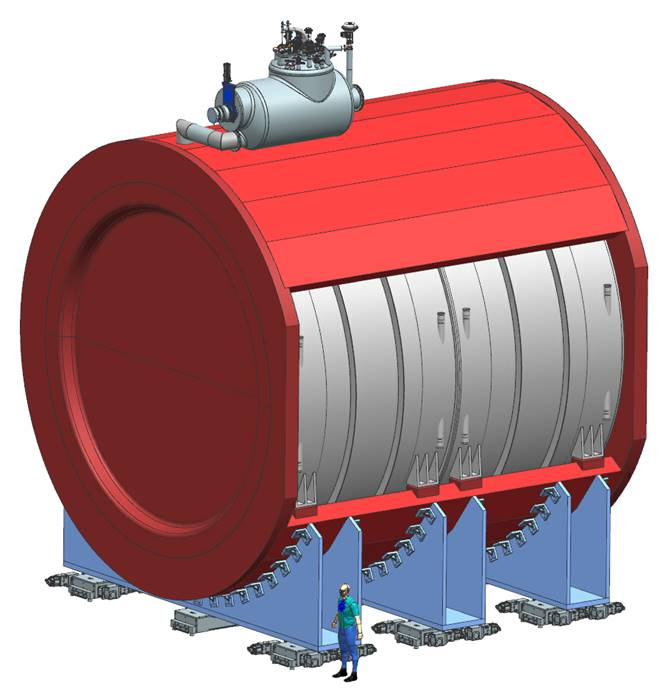
\includegraphics[width=0.6\textwidth]{figures/ch3-DUNE/Spy.jpg}
     \caption{Schematic representation of ND-GAr experiment with its main components}
        \label{fig:Spy}
\end{figure}

\subsection{The SPY magnet system}
The current integrated design for ND-GAr's solenoid, pressure vessel and yoke is named the Solenoid with Partial return Yoke (SPY) \cite{Bersani:2023rlw} and is largely based on the magnet system developed for the Multi Purpose Detector (MPD) at the NICA Collider at JINR \cite{Golovatyuk:2016zps}. The magnet system is composed of a superconducting magnet surrounded by an iron return yoke. To reduce dimensions and overall costs, the magnet and cryostat system has been designed to serve as the cylindrical component of the pressure vessel for the HpGTPC, while also providing support for the HpGTPC and the ECAL, which will be fully contained inside its volume.

The magnet coil is composed of rectangular superconducting cables bent and grouped to form six identical sub-coils with an internal diameter of 7 m, a length of 0.9m and a thickness of 20 mm, operating at 5000A. The coils will be hosted in a cryostat reaching operating temperatures of 4.5 K to 4.7 K. The cooling elements of the cryostat will consist of pipes welded onto the outer surface of the coil formers hosting a thermosiphon-driven flow of liquid helium. 

SPY's magnet will produce an overall magnetic field of 0.5T with a field uniformity of $\pm 1\%$. These field characteristics surpass the requirements necessary to achieve the particle reconstruction performance desired by ND-GAr. These include a minimum 3\% momentum resolution for muons exiting from ND-LAr and a performance at least as good as the Far Detector for particles produced in neutrino interactions on gas. The yoke has also been designed to reduce the amount of material between ND-LAr and ND-GAr to a minimum by removing a portion of the downstream barrel. This is important to ensure that the muons coming from ND-LAr loose as little energy as possible in un-instrumented portions of the detectors, reducing the relative uncertainties to a minimum.

SPY is completed by a carbon steel return yoke, which presents several unique characteristics. The pole faces of the yoke have been designed to offer sufficient mechanical strength to act also as the end-caps of the detector's pressure vessel. This removes the necessity for the large domed heads that would normally be required for a pressure vessel of such a diameter, shortening the overall dimensions of the system by about 4m.

\section{The temporary muon spectrometer}
\clearpage

\section{The temporary muon spectrometer}
\subsection{ND-GAr-Lite}
\subsection{TMS}
\section{Dune's scientific program}
\subsection{Sensitivities and systematics}
\subsection{Mass ordering and $\delta_\textrm{CP}$}
\subsection{Precision measurements}
\subsection{Proton decay}
\subsection{Supernova neutrinos}
\subsection{Oscillation physics with atmospheric neutrinos}
\subsection{Near Detector Physics}
%\subsection{ND-GAr Physics}
% \begin{savequote}[8cm]
% La fisica è diventata così potente e ricca da poter nuovamente introdurre nei propri modelli la complessità e il disordine, ciò che Galileo era stato costretto a escludere.

% Physics has become so powerful and rich to be able to re-introduce complexity and disorder in its models, which is what Galileo was forced to leave behind.
% \qauthor{--- Giorgio Parisi}
% \end{savequote}


\chapter{\label{ch:4-KF-NDGArLite}Kalman Filter reconstruction for ND-GAr-Lite}
\minitoc

\section{Introduction}
ND-GAr-Lite was a proposed temporary muon spectrometer  for the DUNE ND complex, to be used during Phase-I of the experiment. As described in Sec. \ref{Sec: DUNE-GArLite} the key design principle behind the detector was to include the structural components of ND-GAr, but to exclude the active detector elements: the gas TPC and the ECAL. In their place a simple tracker composed of segmented tracking planes would be built. Significant effort was dedicated to this design by the ND-GAr group, which was able to produce official geometries for the detector and code which allowed to fully simulate the passage of particles through it, down to the signal formation, and track finding and reconstruction.

While a full simulation for ND-GAr-Lite was available at the time of the writing of this thesis, it was known that many aspects were not mature. In particular the track reconstruction algorithm was known not to be at a state-of-the-art level. No treatment of energy loss or multiple scattering was put in place and no estimate of the uncertainties from the measurement was produced by the algorithm.

As a key part of this thesis project, a collaboration with experts from the ALICE experiment tracking group was established to produce a Kalman Filter based on the one used for the ALICE TPC (see Chapter \ref{ch:5-KF-NDGArToy} for a full description). This new algorithm was set to improve on the existing one and fit the needs of both the new geometry of the ALICE detector as well as ND-GAr. In this context, an additional goal of this thesis project became to produce a similar algorithm, also based on the pre-existing ALICE Kalman Filter, that could be applied to ND-GAr-Lite's tracker. 

The first step in the development of the algorithm, consisted in creating a simple Toy Monte Carlo simulation which allowed for a high degree of control over many aspects of particle propagation and signal formation. This was achieved by developing many aspects of the simulation modularly and somewhat independently from one another. Most of the development stage in the algorithm's life consisted in producing different samples with this Toy Monte Carlo tool and then testing the performance of the algorithm and whether it conformed to expectations. Once the Kalman Filter was thought to be at a good level of maturity, it was tested on the more complete simulation already available from the ND-GAr group.

This Chapter will be divided as follows: in Sec. \ref{Sec:KalmanTheory} we give a brief overview of the Kalman Filter technique as it applies to track fitting; in Sec. \ref{Sec:KFLite} we introduce the Kalman Filter algorithm developed for ND-GAr-Lite; in Sec. \ref{Sec:GArSoft_Lite} we give a full description of the simulation software developed by the ND-GAr group; in Sec. \ref{Sec:ToySim-Lite} we describe the Toy Monte Carlo tool specifically developed for the testing of the Kalman Filter; in Sec. \ref{Sec:ToyMCTests-Lite} we present some selected results from the tests done using the Toy Monte Carlo tool; in Sec. \ref{Sec:MC-Studies-Lite} we show the performance of the algorithm when applied to the more complete simulation developed by the ND-GAr group and we compare with the results obtained with the previously existing algorithm.

\section{The Kalman Filter technique}
\label{Sec:KalmanTheory}
In this section we offer a brief review of the Kalman Filter technique, specifically in the context of track fitting~\cite{Bishop1995,Kalman_app}. 
Track fitting consists in estimating track parameters, while filtering involves analyzing linear dynamic systems. By viewing a track in space as a dynamic system, we can utilize filtering techniques for track fitting, including Kalman Filters. This can be achieved by uniquely describing the conditions of the particle with a number of parameters grouped into a true state vector, $s^{\textrm{true}}$ (a function of a suitable coordinate, $x_k$, known as the free parameter) at each trajectory point $k$, $s^{\textrm{true}}(x_k) \equiv s_k^{\textrm{true}}$. 

Assuming that the system is linear, the propagation of $s_k^{\textrm{true}}$ can be described by a linear transformation, $F_{k}$. The propagation of the system can be corrupted by inherent processes, such as multiple scattering for a charged particle moving across a medium. This random disturbance can be encapsulated in a process noise vector, $w_k$, and can affect all or only some of the state vector variables. The propagation of the system can then be written as:
\begin{equation} \label{eq:ev}
     s_k^{\textrm{true}} = F_{k-1}s_{k-1}^{\textrm{true}}+w_{k-1}.
\end{equation}

By using a detector we are able to measure some properties of the particle at specific intervals of $x_k$, where the trajectory and the detector intersect. We can encapsulate these properties in a measurement vector,  $m_k$, which is a linear combination of the properties in $s_k^{\textrm{true}}$. If the detection process is affected by noise, $m_k$ will also be corrupted by a measurement noise vector, $\epsilon_k$. The whole measurement operation can be written as :
\begin{equation}
    m_k = H_k s_k^{\textrm{true}} + \epsilon_k,
\end{equation}
where $H_k$ is a linear transformation. 

We assume that all components of $w_k$ and $\epsilon_k$ are Gaussian distributed, unbiased, and uncorrelated. The expectation values and covariances for the $k^\textrm{th}$ are defined as:
\begin{align}
    \text{E}\left[w_k\right]&=\vv{0}, \;\text{Cov}\left[w_k\right]=Q_k, \\  
    \text{E}\left[\epsilon_k\right]&=\vv{0}, \;  \text{Cov}\left[\epsilon_k\right]=R_k.
\end{align}
The Kalman Filter is a Bayesian iterative algorithm which produces an estimate,  $s_k$, of the true state vector, $s_k^{\textrm{true}}$, at each trajectory point. It combines \textit{a priori} knowledge of the system, condensed in the track propagator, $F_k$, and the measurement information from $m_k$. The covariance matrix associated with the estimated state vector, $s_k$, is defined as:
\begin{equation} \label{eq:covdef}
    \text{Cov}\left[s_k\right] = C_k.
\end{equation}
The Kalman Filter procedure can be divided into discrete operational steps, that are applied iteratively:
\begin{enumerate}
    \item Seeding: Produce an initial estimate for the state vector and covariance matrix, $s_0$ and $C_0$, respectively, using a certain technique.
    \item Propagation: Produce an \textit{a priori} estimate for the state vector and the covariance matrix, $\widetilde{s}_k$ and $\widetilde{C}_k$, respectively, at the next $x_k$ ($k\ge1$) step, using only the track propagator and no measurement knowledge:
    \begin{align}
        \widetilde{s}_k&=F_{k-1}s_{k-1},\label{eq:prop} \\
        \widetilde{C}_k&=F_{k-1}C_{k-1}F_{k-1}^T+Q_{k-1},\label{eq:pcov}
    \end{align}
    where the process noise matrix $Q_k$ is added as a correction to the covariance matrix. Note that $T$ stand for transpose.
    \item Update: Produce an updated estimate for the state vector and the covariance matrix, $s_k$  and $C_k$, respectively, using information from the current measurement. The update is performed requiring that the covariance for the new estimate is minimized. This is done through the use of the so called Kalman gain, which is defined as:
    \begin{equation}
        K_k\equiv\widetilde{C}_k H_k^T\left(R_k+H_k \widetilde{C}_k H_k^T\right)^{-1}.\label{eq:kgain}
    \end{equation}
    The update operation, also known as filtering, then follows as:
    \begin{align}
        s_k&=\widetilde{s}_k+K_k\left(m_k-H_k \widetilde{s}_k\right),\label{eq:updates}\\
        C_k&=\left(\mathbb{1}-K_kH_k\right)\widetilde{C}_k.\label{eq:updatec}
    \end{align}
 To proceed to the next point, the algorithm is repeated from the propagation step, using the current updated estimate, $s_k$, as the input. 
\end{enumerate}
An illustration of the basic functioning of the Kalman Filter algorithm is provided in Fig.~\ref{fig:KFdiagramfinal}.

\begin{figure}[t]
     \centering
     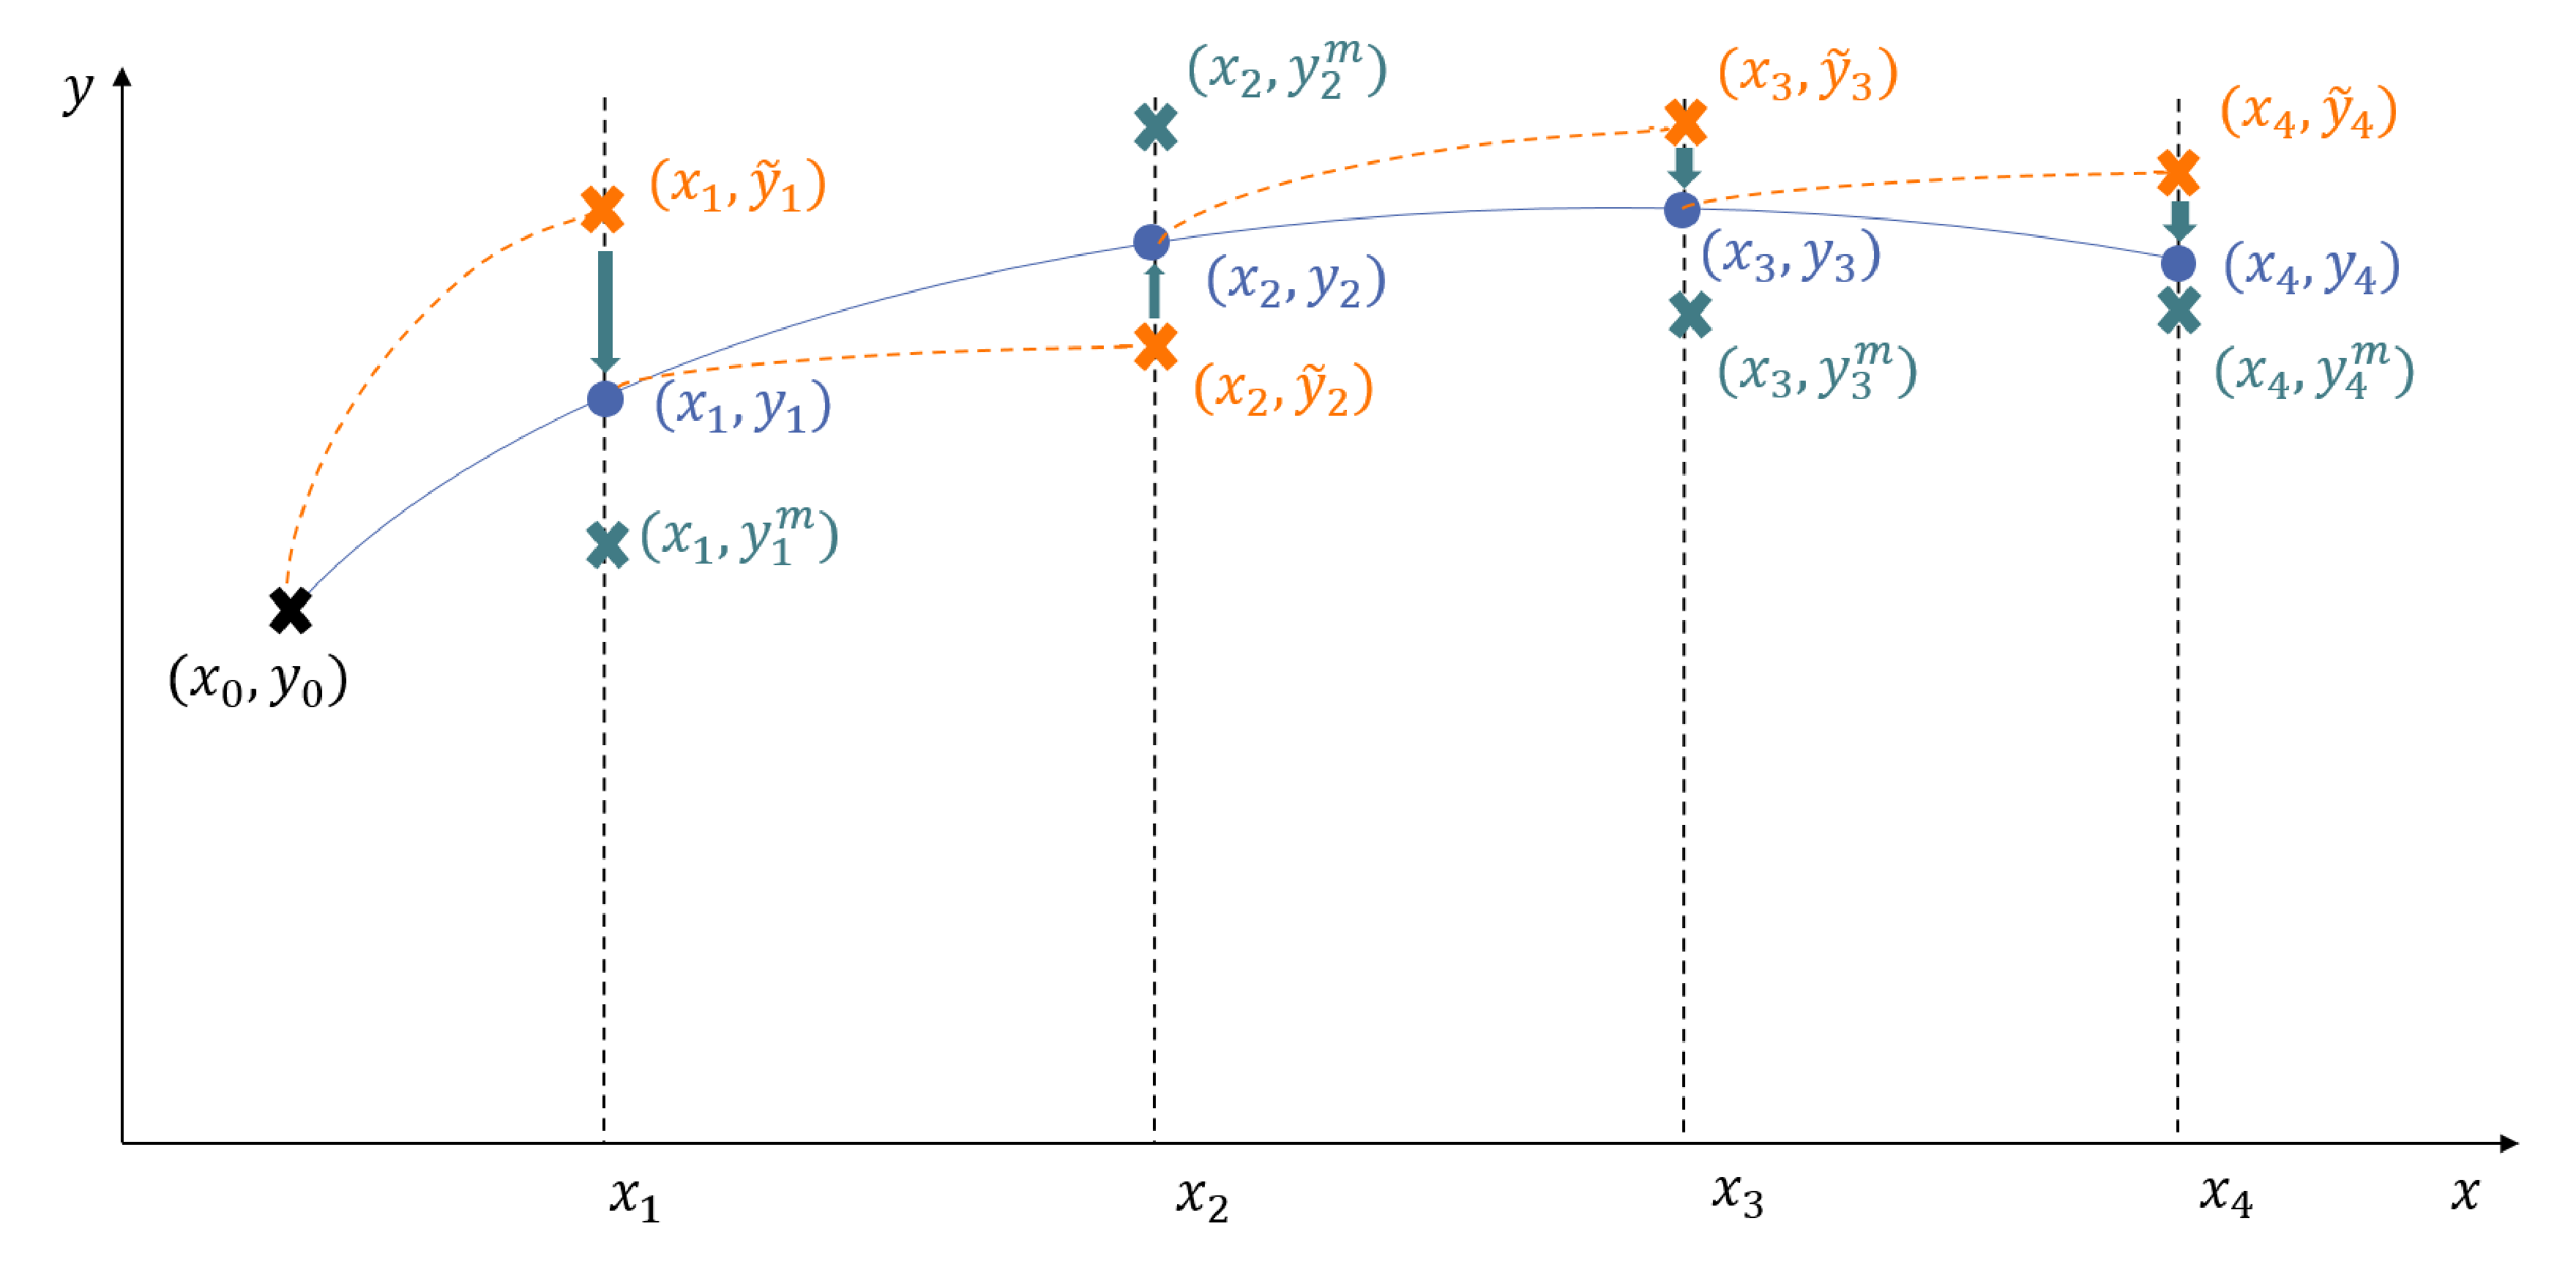
\includegraphics[width=0.99\textwidth]{figures/ch2-Theory/KFdiagram_final.eps}
     \caption[Schematic representation of a Kalman Filter]{Schematic representation of a Kalman Filter: $y$ represents one of the variables of the state vector $s$ which is a function of the free parameter $x$. The coordinates of the free parameter $x_k$ are taken at the points of intersection between the detector and the particle trajectory. Starting from the first estimate $(x_0,y_0)$, which is obtained from a seeding algorithm, the Kalman Filter produces an \textit{a priori} estimate at the following point $(x_1,\widetilde{y}_1)$, shown in orange. The result is compared with the measurement $(x_1,y_1^\textrm{m})$ shown in green and the filtering step is applied, producing an updated estimate $(x_1,y_1)$. The procedure is repeated until no more track points are available \cite{Battisti:2024nqq}.}
        \label{fig:KFdiagramfinal}
\end{figure}

The machinery described so far, assumes that the evolution of the dynamic system is determined by linear transformations. However, the propagation of a charged particle in a magnetic field is non-linear. Equation~\ref{eq:prop} in this case takes the more general form:
\begin{equation}\label{eq:EKF}
    \widetilde{s}_k=f_{k-1}\left(s_{k-1}\right),
\end{equation}
where $f_{k-1}$ is a non-linear function. In order to apply the Kalman Filter technique, the track propagator in Eq.~\ref{eq:pcov}, $F_{k-1}$, has to be approximated by the Taylor expansion coefficient defined as follows:
\begin{align}
    f_{k-1}\left(s^*\right)& \simeq f_{k-1}\left({s}_{k-1}\right) + F_{k-1}\cdot\left(s^*-{s}_{k-1}\right), \label{eq:jacobian} \\
    F_{k-1}&=\frac{\partial f_{k-1} }{ \partial s^*},\label{eq:jacobian2}
\end{align}
where $s^*$ is a generic state vector coordinate near the point of expansion, $s_{k-1}$. All the other Kalman Filter steps (Eqs.~\ref{eq:kgain}-\ref{eq:updatec}) remain identical to the linear procedure. This technique is known as extended Kalman Filter. 

\section{The Kalman Filter applied to ND-GAr-Lite}
\label{Sec:KFLite}
The Kalman Filter developed for ND-GAr-Lite was largely based on the parametrization utilized by the ALICE collaboration for their own TPC Kalman Filter, which can be considered the state of the art in the field ~\cite{Ivanov:2003yr, Arslandok:2022dyb}. The code produced to apply and test the custom Kalman Filter, however was largely produced as a custom tool to accommodate the peculiarities of ND-GAr-Lite's tracking system which has little in common with a gas TPC such as ALICE. The Kalman Filter algorithm developed for ND-GAr-Lite will be referred to as \texttt{KF-Lite}. 

We assume that an ideal magnetic field is applied along the direction perpendicular to the neutrino beam which is identified by the coordinate $z$. The $x$ coordinate identifies the horizontal direction, while the $y$ coordinate identifies the vertical.  The spatial information in the $zy$ plane is assumed to be given by the detector's tracking planes. The information regarding the $x$ coordinate is given by the central position of the triangular scintillator bar in which the hit was formed.

\begin{figure}[!ht]
         \centering
         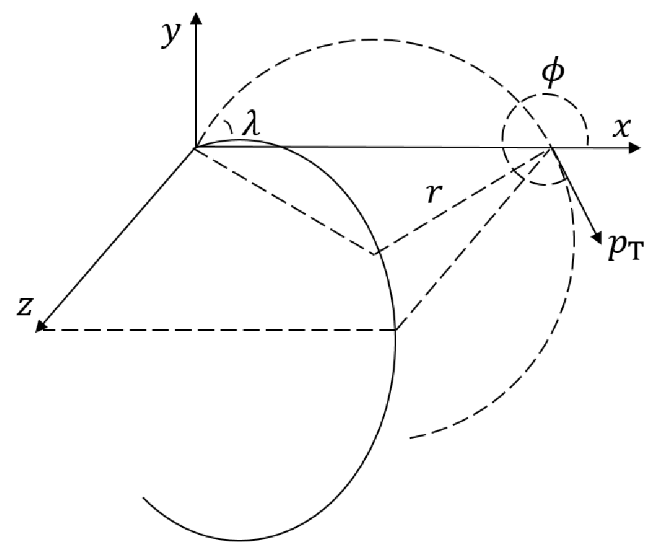
\includegraphics[width=0.6\textwidth]{figures/ch4-KF_NDGArLite/Variables_Diagram_new.png}
        \caption[Diagram illustrating the definition of the coordinates defining the evolution of the custom Kalman Filter.]{Diagram illustrating the definition of the coordinates defining the evolution of the custom Kalman Filters produced for ND-GAr-Lite as well as ND-GAr. } \label{fig:Detector_var}
\end{figure}


The algorithm is evolved along the free parameter, $x$, and its state vector is defined as:
\begin{equation}\label{eq:state}
    s(x) = \left(y,z,\sin{\phi},\tan{\lambda}, q/p_{\text{T}}\right),
\end{equation}
where $y$ is the vertical direction; $z$ is the drift direction; $\phi$ is the azymuthal angle of the transverse momentum i.e. the component of the momentum vector transverse to the drift direction; $\lambda$ is the ``dip angle''  between the transverse momentum and the total momentum vector; q is the charge sign of the particle and $p_{\text{T}}$ is the module of the transverse momentum. Note that the inverse transverse momentum can also be written in terms of track curvature $1/r$. The conversion is easily obtained using the standard formula for charged particles moving in a magnetic field:
\begin{equation}\label{eq:curvatureconv}
    p_{\text{T}} \ \left(\text{GeV}/c\right) =0.3 \ B \left(\text{T}\right) \ r \left(\text{m}\right).
\end{equation}
A visual representation of the coordinates is given in Fig.~\ref{fig:Detector_var}.

The state vector is evoleved along the trajectory using a propagator function, as described in Eq. \ref{eq:prop}:
\begin{equation} \label{eq:func}
    \widetilde{s}_k = f_{k-1}(s_{k-1}) =
        \left\{
        	\begin{aligned}
        		& \widetilde{y}_k  =  y_{k-1}+ \frac{\sin{\phi}_{k-1}+\sin\widetilde{\phi}_k} 
                                     {\cos{\phi}_{k-1}+\cos\widetilde{\phi}_k}  \Delta x_k,  \\
        		& \widetilde{z}_k  =  z_{k-1}+\left(\widetilde{\phi}_k-\phi_{k-1}\right)\frac{r}{q}_{k-1}\tan{\lambda}_{k-1} ,\\ 
                    & \sin \widetilde{\phi}_k =  \sin \phi_{k-1} + \frac{q}{r}_{k-1}\Delta x_k,  \\               
                    & \tan \widetilde{\lambda}_k   =  \tan \lambda_{k-1}, \\   
                    & \widetilde{\frac{q}{p_{\text{T}}}}_k = \frac{q}{p_{\text{T}}}_{k-1} \times\frac{p_{k-1}}{\Delta p_k+p_{k-1}},
        	\end{aligned}
        \right.
\end{equation}
where $\Delta x_k$ is the distance in the $x$ direction between the previous and current points, $p_k$ is the total momentum and $\Delta p_k$ is the total momentum loss. In order to obtain the propagation matrix, $F_k$, one only needs to calculate the Taylor expansion coefficient $\partial f_k / \partial s_k$, as described in Eqs. \ref{eq:jacobian} and \ref{eq:jacobian2}, with the exception of the $q/p_{\text{T}}$ term, which is treated separately.

In order to compute the momentum loss, $\Delta p_k$, at each trajectory point, the ionization energy loss, $-\textrm{d}E/\left(\rho\textrm{d}x\right)$ (where $\rho$ is the density of the material in $\text{g/cm}^3$), of the particle is evaluated using the standard Bethe-Bloch formula as defined in Eq. \ref{eq:Bethe}.
%~\cite{PDG}:
% \begin{equation} \label{eq:Bethe}
%     -\frac{\textrm{d}E}{\rho\textrm{d}x} = 4\pi N_{A}r_e^2m_ec^2z^2\frac{Z}{A}\frac{1}{\beta^2}\left(\frac{1}{2}\ln{\frac{2m_ec^2\beta^2\gamma^2T_{\textrm{max}}}{I^2}}-\beta^2-\frac{\delta}{2}\right),
% \end{equation}
% where $N_{A}$ is Avogadro's number, $r_e$ is the classical electron radius, $m_ec^2$ is the electron mass energy, $z$ is the charge of the particle, $Z$ and $A$ are the atomic number and mass of the absorbing material, $\beta$ and $\gamma$ are the usual relativistic factors for the passing particle, $I$ is the material mean excitation energy, $T_{\textrm{max}}$ is the maximum kinetic energy which can be imparted to a free electron in a single collision and $\delta/2$ is a density effect correction factor. 
The differential energy loss, $-\textrm{d}E/\left(\rho\textrm{d}x\right)$, is calculated using the properties of the most abundant gas present in the gas mixture in standard conditions and then multiplied by the material's density to obtain a reasonable approximation of the $\textrm{d}E/\textrm{d}x$~\cite{STERNHEIMER1984261}. The total momentum loss between two steps is then calculated by numerical integration~\cite{Griffiths2010}. 

In the evaluation of $F_k$, the $q/p_{\text{T}}$ parameter is treated as if it were static. A correction term, $c_k$ is added to the $q/p_{\text{T}}$ diagonal element of the covariance matrix, $\widetilde{C}_k$, after the propagation step:
\begin{equation} \label{eq:eloss-factor}
    c_k=\left(a\cdot\frac{\Delta p_k}{p_{k-1}} \cdot\frac{q}{p_{\text{T}}}_{k-1}\right)^2,
\end{equation}
where $a=3.162\times 10^{-3}$ is a constant multiplicative factor which is directly taken from the ALICE TPC framework~\cite{carminati2003simulation}.

Multiple scattering is treated through the noise correction matrix, $Q_k$. At each step the scattering angle can be treated as emerging from a Gaussian distribution with a root mean square equal to the Molière angle $\theta_{\textrm{M}}$, as defined in Eq. \ref{eq:MoliereAngle}. The $Q_k$ terms relative to $\sin \phi$, $\tan \lambda$ and $q/p_{\text{T}}$ are evaluated through error propagation and added to the covariance matrix as described in Eq. \ref{eq:pcov}:
\begin{equation}\label{eq:Q}
    Q =\begin{bmatrix}
    0 & 0 & 0 & 0& 0 \\
    0 & 0 & 0 & 0& 0 \\
    0 & 0 & \theta_{\textrm{M}}^2\cdot\frac{\cos^{2}\phi}{\cos^{2}\lambda} & 0& 0 \\
    0 & 0 & 0 & \frac{\theta^2_{\textrm{M}}}{\cos^4\lambda}& \frac{q}{p_{\text{T}}}\cdot\theta^2_{\textrm{M}}\cdot\frac{\tan\lambda}{\cos\lambda} \\
    0 & 0 & 0 & \frac{q}{p_{\text{T}}}\cdot\theta^2_{\textrm{M}}\cdot\frac{\tan\lambda}{\cos\lambda}& \left(\frac{q}{p_{\textrm{T}}}\right)^2\theta^2_{\textrm{M}} \tan^2\lambda
    \end{bmatrix} .
\end{equation}

Note that in the case of ND-GAr-Lite the material budget corrections are applied only between points that are inside the same tracking plane. When the \texttt{KF-Lite} needs to be moved between two consecutive points which lie in separate planes, the state vector is propagated in three separate steps: first the state vector is propagated to the edge of the first plane and the correspondent material budget corrections are applied; then it is propagated to the next plane applying no corrections, since the space between the planes is considered to be empty; finally the state vector is propagated to the following point and both the material budget corrections and the filtering step of the \texttt{KF-Lite} algorithm are applied.

Each step in the evolution of the \texttt{KF-Lite} can potentially fail, in which case the algorithm is stopped. This can happen mainly in two scenarios: $\sin \phi$ can be calculated to be out of range, i.e. $|\sin \phi|>(1-10^{-7})$ or the particle can lose all its remaining energy. Once the \texttt{KF-Lite} is stopped, the information for each of the reconstructed points is saved. Flags are used to preserve information on which of the reconstruction steps have been successful and which have failed.


\subsection{Seeding algorithms}
\label{Sec:SeedingLite}
One of the limitations of the Kalman Filter technique is that it requires an initial estimate to be externally provided, both for the state vector $s_0$ and the covariance matrix $C_0$. As mentioned in
Sec. \ref{Sec:KalmanTheory} this procedure is often referred to as \enquote{Seeding} and the initial estimates are referred to as the algorithm’s \enquote{Seed}. Two seeding methods have been tested for this work: the first is taken directly from the ALICE infrastructure, while the second coincides with the algorithm originally used by ND-GAr-Lite for its track reconstruction.

The seeding strategy originally used by the ALICE experiment consists in a simple three-point circle finding algorithm and will be referred to from now on simply as \texttt{Seed}. In the plane perpendicular to the magnetic field, the trajectory of a charged particle is a circle. Since only one circumference will pass through any three points, one can find a point which is roughly at the start of the particle trajectory, one at the end and one in the middle and obtain the properties of the circle that passes though them. This equates to solving a system of three linear equations for three unknown variables: the coordinates of the center of the circumference $(x_C,y_C)$ and its radius $r$. After traslating the coordinate system to the first of the three points $(x_0,y_0)$ the equations can be written as:
\begin{equation}
\begin{cases} 
x_C^2+y_C^2 = r^2, \\
(x_1-x_C)^2+(y_1-y_C)^2=r^2, \\
(x_2-x_C)^2+(y_2-y_C)^2=r^2,
\end{cases}
\end{equation}
where $(x_C,y_C)$ and $(x_n,y_n)$ are the traslated center of the circle and the three trajectory points respectively and $r$ is the radius. From the circle properties $(x_C,y_C)$ and $r$ and the coordinates of the three points, one can find an estimate for the state vector $s_0$ at the starting point $(x_0,y_0,z_0)$. Apart from $y_0$ and $z_0$ which are taken as the measured values the other elements are estimated as:
\begin{equation}\label{eq:SeedPar}
    \begin{cases}
        1/p_\textrm{T} = 1/(0.3  B  r )\\
        \sin \phi = x_C/r \\
        \tan \lambda = z_1 / \Delta xy
    \end{cases}
\end{equation}
where $\Delta xy$ is the arch between the first and second point and is calculated as:
\begin{equation}
    \Delta xy = 2r \arcsin \left( \frac{\sqrt{y_1^2+x_1^2}}{2r}\right)
\end{equation}
The charge sign $q$ is determined as:
\begin{equation}
    q = \frac{x_3y_2-x_2y_3}{|x_3y_2-x_2y_3|}
\end{equation}
The three-point method for the estimation of the initial-state vector $s_0$ can be written as: 
\begin{equation}
    s_0 = h\left[\left(x_0,x_1,x_2);(y_0,y_1,y_2,z_0,z_1, z_2\right)\right]\equiv h(\zeta;\eta) ,
\end{equation}
where $x_i,y_i$ and $z_i$ are the measured coordinates of the three points, all taken to be independent and uncorrelated. In order to compute an estimate for $C_0$ one can use the matrix expression for error propagation~\cite{Cov}:
\begin{equation}\label{eq:error_Prop}
    C_0 = gVg^T 
\end{equation}
\begin{equation}
   g_{ij}  = \frac{\partial h_i}{\partial \eta_j},
\end{equation}
where $V$ is the covariance matrix of the vector $\eta$, which is determined by the resolution of the detector in $y$ and $z$. The coordinate $x$ is taken to be the free parameter and thus is not considered in the error propagation. The partial derivatives are estimated numerically as:
\begin{equation}
    \frac{\partial h_i}{\partial \eta_j} \approx \frac{h(\zeta;\eta_{i\neq j},\eta_j+\sigma_{\eta_j})-h(\zeta;\eta_{i\neq j},\eta_j)} {\sigma_{\eta_j}},
\end{equation}
where $\sigma_{\eta_j}$ is the resolution of the vector element $\eta_j$. The \texttt{Seed} estimation for both the covariance matrix $C_0$ and the state vector $s_0$ is adjusted for energy loss and multiple scattering using the same method as the Kalman Filter. The $q/p_\texttt{T}$ ratio is corrected with the factor described in Eq.~\ref{eq:func}, and the relative covariance matrix element is updated by adding the $c_k$ factor from Eq.~\ref{eq:eloss-factor}. To handle multiple scattering, the $Q$ matrix calculated in Eq.~\ref{eq:Q} is added to the covariance. The total distance traveled, needed to calculate total energy loss and the scattering angle $\theta_\texttt{M}$, is determined by determining the length of the trajectory of the particles which is confined inside the scintillating planes. 

The second seeding algorithm consists in the iterative linear regression method for circle fits (\texttt{ILRM}) outlined in \cite{ILRM}. It was originally used as ND-GAr-Lite's full reconstruction algorithm and has so far only been tested as a seeding method on ND-GAr-Lite. The algorithm is closely related to the least squares method, where the center of the circle trajectory in the $xy$ plane and its radius $r$ are found by minimizing the functional:
\begin{equation}
    L(x_C,y_C,r)=\sum_{i=1}^{n}(\sqrt{(x_i-x_C)^2+(y_i-y_C)^2}-r)=\sum_{i=1}^{n}\rho_i
\end{equation}
where $(x_i,y_i)$ are the coordinates of all the points along the track. Due to the non-linear dependence of the functional $L$ on the circle parameters, applying the least square method leads to very cumbersome computations. One can then linearize the system by introducing the new variable $Z_i=x_i^2+y_i^2$ and re-writing the circle equation as:
\begin{equation}
    Z = 2x_Cx+2y_Cy+\gamma
\end{equation}
where $\gamma = r^2-x_C^2-y_C^2$. This linear regression method (LRM) is equivalent to minimizing the functional:
\begin{equation}
    M(x_C,y_C,r)=\sum_{i=1}^{n}((x_i-x_C)^2+(y_i-y_C)^2-r^2)^2
\end{equation}
While the LRM method is much faster than the non-linear method, it is only reliable in the cases where $\rho_i\ll r$. The \texttt{ILRM} method solves this instability issue by utilizing a slightly different functional:
\begin{equation}
    \label{eq:ILRMfunctional}
    K(x_C,y_C,r)=M(x_C,y_C,r)r^{-2}
\end{equation}
Using the numerical methods outlined in App. \ref{App:ILRM}, it is possible to find values of $(x_C,y_C,r)$ which minimize $K$,  maintaining the computational agility of the LRM method, and the stability of the non-linear methods. 

Starting from the circumference properties, all the components of the state vector can be calculated as described in Eq. \ref{eq:SeedPar}. The covariance matrix $C_0$ is estimated as in Eq. \ref{eq:error_Prop}, reapplying the fit only to three points, at the start, end and middle of the particle trajectory. This approximation is not completely correct and tends to overestimate the uncertainties, since in reality, all the points in the track are used. However, since only a rough estimate of $C_0$ is needed by the \texttt{KF-Lite}, no other method has been explored. As in the case of the application of the ALICE algorithm to ND-GAr-Lite, only the diagonal elements of $C_0$ are considered.
\section{The ND-GAr software suite: \texttt{GArSoft}}
\label{Sec:GArSoft_Lite}
\texttt{GArSoft} is a software toolkit used to handle the simulation and reconstruction of events inside ND-GAr and ND-GAr-Lite \cite{garsoft}. It is largely based on the \texttt{LArSoft} toolkit \cite{Church:2013hea,LArSoft} which is used by the DUNE experiment to handle the simulation and reconstruction for all its liquid argon based detector i.e. the ND-LAr detector and the FD modules. \texttt{GArSoft} as well as \texttt{LArSoft} are based on the \texttt{art} event processing framework \cite{Green:2012gv}, which is shared by most of the modern Fermilab experiments. The \texttt{art} framework allows for the different simulation and reconstruction steps to be handled modularly through the use of simple \texttt{fcl} text files.

\subsection{Particle generation and propagation in \texttt{GArSoft}}
\label{Sec:GArSoft_PartGen}
In \texttt{GArSoft} the simulation of neutrino interactions inside the detector geometries is handled through the use of the Generator of Events for Neutrino Interaction Experiments (GENIE) \cite{Andreopoulos:2009rq}. The main component of GENIE is the GENIE Generator, which provides software tools which support a state-of-the-art comprehensive physics model for neutrino interaction simulations in realistic experimental setups. GENIE also offers extensive data archives to allow for MC/data comparisons as well as a generator tuning framework. GENIE can be used in \texttt{GArSoft} by providing the generator with a neutrino flux file in the form of ROOT \cite{Brun:1997pa} n-tuples, a detector geometry in the form of a ROOT-readable \texttt{gdml} file and by specifying the type of neutrino interaction that one wants to simulate as well as the portion of the detector geometry in which the the user desires the interaction to occur. This framework allows for the neutrino interaction generation to be handled identically independently from the detector that one wants to simulate, assuming that the correct \texttt{gdml} file is provided. 

In addiction to the GENIE event generator, \texttt{GArSoft} also supports a particle gun generator. This tool allows the user to generate individual particles inside the detector geometry, specifying their type, starting position, 3-dimensional momentum and energy. This particle gun tool is directly adapted from Geant4 \cite{GEANT4:2002zbu}. Geant4 is a software package composed of tools for the simulation of the passage of particles through matter. The toolkit is capable of handling all aspects of the simulation, which include: the geometry of the detector and the materials involved, which in \texttt{GArSoft} are specified through a ROOT-readable \texttt{gdml} file; the fundamental particles of interest and the tracking of particles through materials and electromagnetic fields; the physics processes governing particle interactions as well as the response of sensitive detector components; the generation of event data, the storage of events and tracks, the visualization of the detector and particle trajectories, and the capture and analysis of simulation data at different levels of detail and refinement. 
\begin{figure}[t]
     \centering
     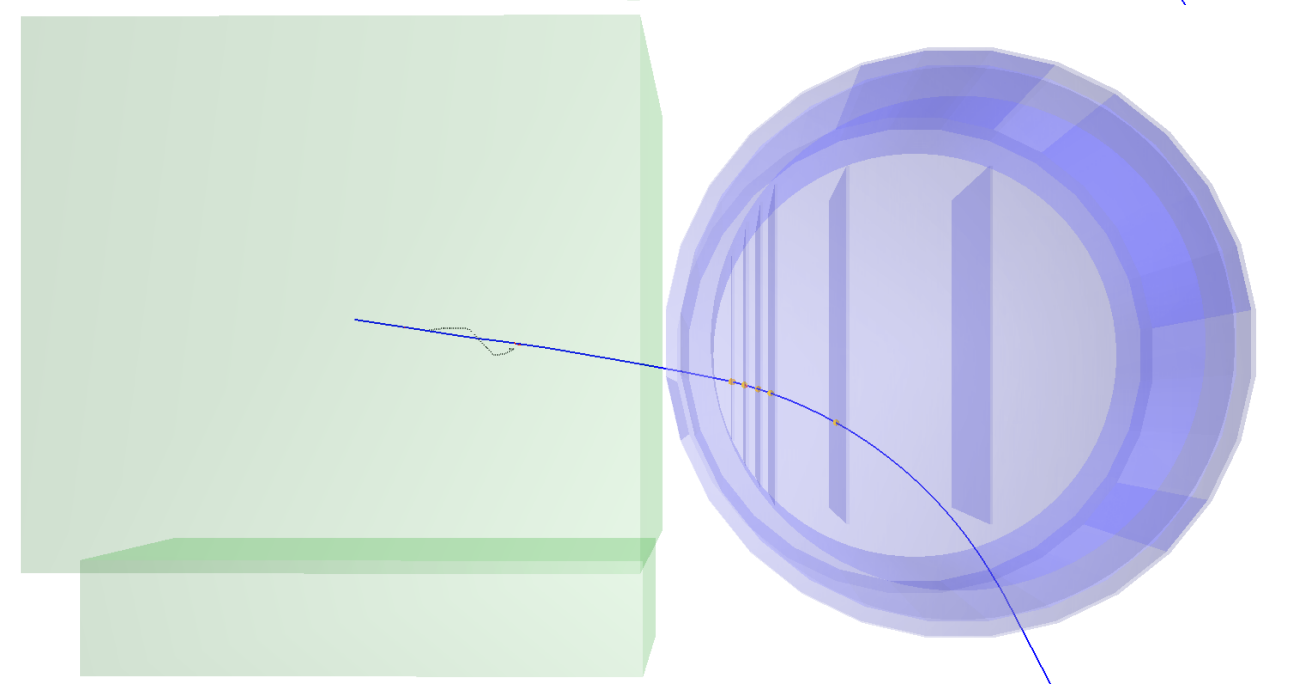
\includegraphics[width=0.9\textwidth]{figures/ch4-KF_NDGArLite/Event_display.png}
     \caption{ND-GAr-Lite tracker station layout with the 6-plane optimized design. The transparent green box depicts ND-LAr with an exiting muon that enters ND-GAr-Lite \cite{ND-GAR-LiteCDR}.}
        \label{fig:EvtDisplayplane}
\end{figure}

In \texttt{GArSoft} Geant4 is used to handle all aspects of the simulation up to the signal formation and digitization step which is handled through custom-made software which is detector-specific. Geant4 is also used in \texttt{GArSoft} to support a simple event-display application. Fig. \ref{fig:EvtDisplayplane} shows an example of a particle-gun generated muon starting in ND-LAr's volume, shown in light green and crossing the whole volume of the 6-plane configuration of ND-GAr-Lite shown in light blue. The energy deposits in the scintillator planes are highlighted in red. 

\subsection{Digitization, track formation and reconstruction in \texttt{GArSoft} for ND-GAr-Lite}
The signal formation on ND-GAr-Lite's scintillator planes is handled through custom-made software integrated in \texttt{GArSoft}. The hit cluster positions are simulated in the scintillator planes by taking the energy
deposits produced by GEANT4 and mapping them onto the correspondent strips. Each plane is formed by two sub-planes, which are segmented either along the y or z direction into triangularly shaped strips. If the strip belongs to the y-segmented sub-plane, the y is given by the center of the strip and the z is taken as the energy deposit’s position, normally smeared according to the strip’s space resolution which is $\sigma_s = 0.3$ cm; vice-versa if the strip belongs to the z-segmented sub-plane. Note that more than a hit per sub-plane per particle track can be produced depending on the trajectory of the particle. For example a particle with a perpendicular trajectory will on average produce two hits per sub-plane. This is a direct consequence of the disposition of the triangular scintillator strips. The energy deposition is converted to photo-electron counts via a simple response function and the timing information is smeared according to the time resolution of the strips. 

To produce a track candidate, the hit clusters are ordered using the time information, then a set of three hit clusters in three separate tracking planes is found, forming the initial track candidate. An \texttt{ILRM} fit is applied to the triplet and hit clusters are added to the track candidate, based on their vicinity to the helix trajectory defined by the fit. Every time a cluster is added, the track is refitted until the final track candidate is produced. All possible triplets are tested until the best track candidate is found. The original track finding algorithm only produced one track candidate per event. The track finding algorithm has been updated as part of this thesis project; now all the points that haven't been added to the main track candidate are collected and a new track candidate is looked for. This process is repeated until no unmatched clusters are left. The clusters that don't pass the \enquote{closeness} criteria with any of the candidate track trajectories are discarded.

Once all the track candidates are formed, they are fitted once again with the \texttt{ILRM} algorithm to provide estimates for the track parameters at both ends of the particle track. These are then saved in the form of 3-dimensional position and momentum together with all the hit cluster points forming the track. The information regarding the Monte Carlo true trajectory and properties of the particle are saved separately. No \enquote{back-tracker} algorithm which could match the ND-GAr-Lite reconstruction results with the MC truth information, was available at the time of the production of this thesis. These had to be matched separately using positional arguments. 

\section{Toy Monte Carlo simulation}
\label{Sec:ToySim-Lite}

A toy Monte Carlo tool was developed to test and study the new custom \texttt{KF-Lite} algorithm. The simulation was constructed with extreme modularity in mind, so that each of its aspects could be tested separately. The simulation procedure for each track can be divided in the following steps:
\begin{enumerate}
    \item \textbf{Definition of a simplified detector geometry.} The cylinder dimensions of the inner tracker region are specified, together with the position, dimensions, resolution  and material properties of the scintillator planes, which are approximately treated as solid rectangular slabs. The space in between the scintillator slabs is considered to be empty.
    \item \textbf{Particle Generation.} A particle is defined by specifying its type, charge, transverse momentum $p_T$, azymuthal angle $\phi$, dip angle tangent $\tan\lambda$ and starting position. From this information, the initial true MC state vector $s_0^t$ is built.
    \item \textbf{Propagation of the particle.} The state vector is propagated as described in Equation \ref{eq:func}. This is done along the x direction in a fixed coordinate frame at 0.25 cm increments. 
    \item \textbf{Application of energy loss and multiple scattering.} The magnitude of the corrections are calculated using the Bethe-Bloch and Molière formulas respectively, analogously to what was described in Sec. \ref{Sec:KFLite}. Note that these corrections are applied only when the particle is moving inside the scintillator planes.
    \item \textbf{Particle stopping.} The propagation is stopped if: the particle reaches the edges of the detector cylinder; the particle gets close enough to the Bragg Peak, that the basic Bethe-Bloch model no longer well describes the energy loss; one of the propagation steps fails.
    \item \textbf{Hit clusters generation}. All points inside the scintillator planes are recorded and grouped. For each scintillator a random amount of the recorded points, between 1 and 4, is saved as the hit clusters. 
    \item \textbf{Simulation of the measurement noise.} Once the hit clusters are generated, the measurement noise is simulated by smearing the $y$ and $z$ coordinates of the trajectory points with Gaussian distribution having a width equal to the resolution of the detector planes. 
\end{enumerate}
Once a track is generated, no additional track finding step is applied and the \texttt{KF-Lite} is applied on top of one of the possible seeding strategies. The energy loss, multiple scattering and point smearing, determine the process and measurement noise of the simulation; they can all be controlled by the user event by event, both in their magnitude and in whether or not they are applied at all. 


\section{The toy Monte Carlo studies}
\label{Sec:ToyMCTests-Lite}
The toy Monte Carlo tool described in Sec. \ref{Sec:ToySim-Lite} was employed to construct several test particle samples used for the development of the \texttt{KF-Lite} algorithm. The tests focused on the reconstruction of forward going muons in the few GeV's range, crossing the full detector, which are the key particle types for ND-GAr-Lite. The first step for each test, consisted in producing a sample of muons to apply the reconstruction to. Each particle would have either a fixed total momentum, or one chosen randomly from a range selected by the user. All particles were simulated to have a forward going momentum, with randomized small $y$ and $z$ components. The initial position could also either be fixed and set in the middle and front of the first scintillator plane, or placed randomly within a fiducial volume. Two different geometries were considered: the nominal 5-planes geometry and an optimized 6-plane geometry, both described in Sec. \ref{Sec: DUNE-GArLite}.

In the toy Monte Carlo simulation for each production, the Energy Loss, Multiple Scattering and measurement smearing could be set by the user independently from one another. Specifically, each of the elements could be switched on and off entirely, a Landau or Gaussian smearing on the energy loss could be applied, and the magnitude of the measurement smearing could be modified. Once the tracks were formed, the reconstruction was applied. For the seeding portion of the algorithm, only the \texttt{Seed} method, described in  Sec. \ref{Sec:SeedingLite} was fully implemented in the toy Monte Carlo tests. Finally the \texttt{KF-Lite} was applied once in the forward direction and once backwards, producing estimates at both ends of the track. For both the seeding and Kalman Filter applications, the Energy Loss and Multiple Scattering corrections could be applied or not, independently from one another. 

The series of independently set conditions just described, generated a vast amount of sample simulation and reconstruction combinations, most of which have been produced and tested. A summary of all the sample combinations considered for ND-GAr-Lite is provided in Tab. \ref{Tab:Lite} in App. \ref{App:Summary_Tables}. 
\begin{table}[t]
    \centering
    \begin{tabular}{||c|c|c|c|c|c|c|c||}
        \hline
        (cm) &  Plane-1&  Plane-2&  Plane-3&  Plane-4&  Plane-5&  Plane-6& Fiducial\\
        \hline
        \hline
        $x_1$ & -307 & -287 & -267 & -247 & -147 & 53 & -317\\
        \hline
        $x_2$ & -303 & -283 & -263 & -243 & -143 & 57 & -307\\
        \hline
        $y_1$ & -133 & -172 & -199.5 & -224.5 & -249.5 & -249.5 & -149.5\\
        \hline
        $y_2$ & 134 & 173 & 200.5 & 225.5 & 250.5 & 250.5 & 150.5\\
        \hline
        $z_1$ &  -300&  -300&  -300&  -300&  -300&  -300 & -200\\
        \hline
        $z_2$ &  300&  300&  300&  300&  300&  300 & 200\\
        \hline
    \end{tabular}
    \caption{Table showing the positions of the edges of the tracking planes in the 6-plane configuration of ND-Gar-Lite as well as the fiducial volume box from which the particles in the Toy Monte Carlo NC and C samples are generated. }
    \label{tab:Lite dimentions}
\end{table}

In this section we focus on two specific tests numbered 13.5c and 13.5.1c in the table. For these two tests the same simulation conditions were applied. We considered a sample of $5\times10^3$ forward going muons with initial momenta distributed uniformly between 0.5 GeV$/c$ and 4 GeV$/c$ inside the 6-plane geometry of ND-GAr-Lite. Their starting positions are distributed inside a block shaped fiducial volume placed immediately in front of the first plane. A summary of the positions of the six planes and of the starting fiducial volume is shown in Table \ref{tab:Lite dimentions}. Note that the coordinate frame has its origin in the center of the tracking section cilinder, which has a radius of 349.9 cm and a length of 669.6 cm. The scintillator planes were simulated to be made of polyvinyltoluene, a plastic polymere scintillator having a radiation length of $X_0 = 42.54 \ \text{cm}$ and a density of $\rho = 1.032 \ \text{g}/\text{cm}^3$. All the scintillator planes are set to have equal spacial resolution resolution in both the $y$ and $z$ direction of $\sigma_{yz} = 0.3 \ \text{cm}$. 

\begin{figure}[t]
     \centering
     \begin{subfigure}[b]{0.48\textwidth}
         \centering
         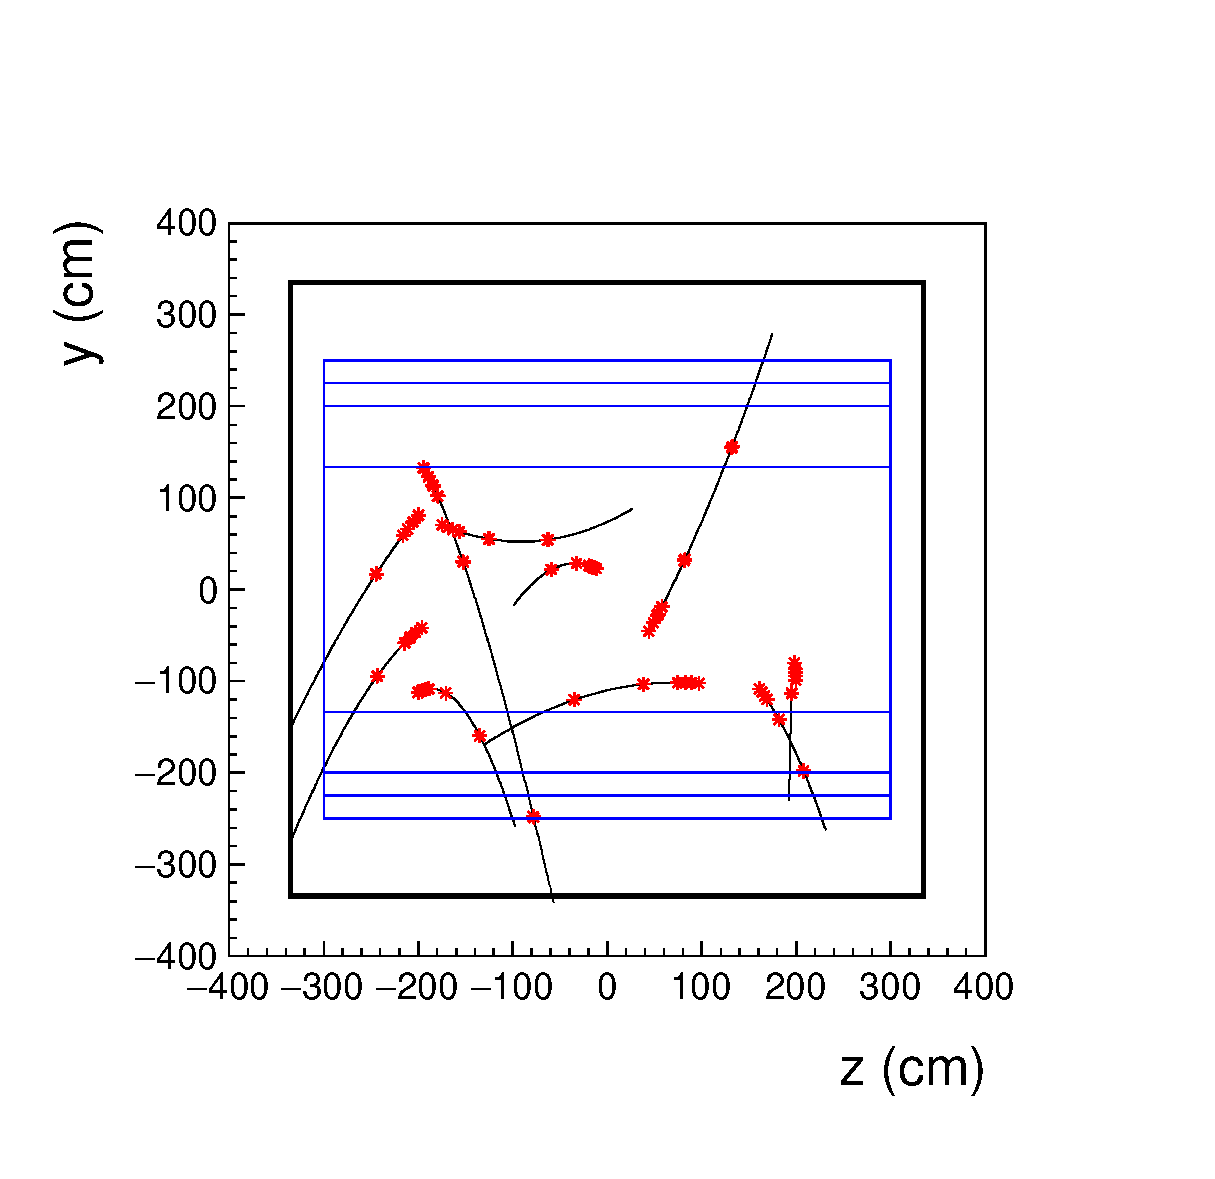
\includegraphics[width=\textwidth]{figures/ch4-KF_NDGArLite/Toy/YZ_view.eps}
         \caption{}
         \label{fig:YZViewGArLite}
     \end{subfigure}
     \begin{subfigure}[b]{0.48\textwidth}
         \centering
         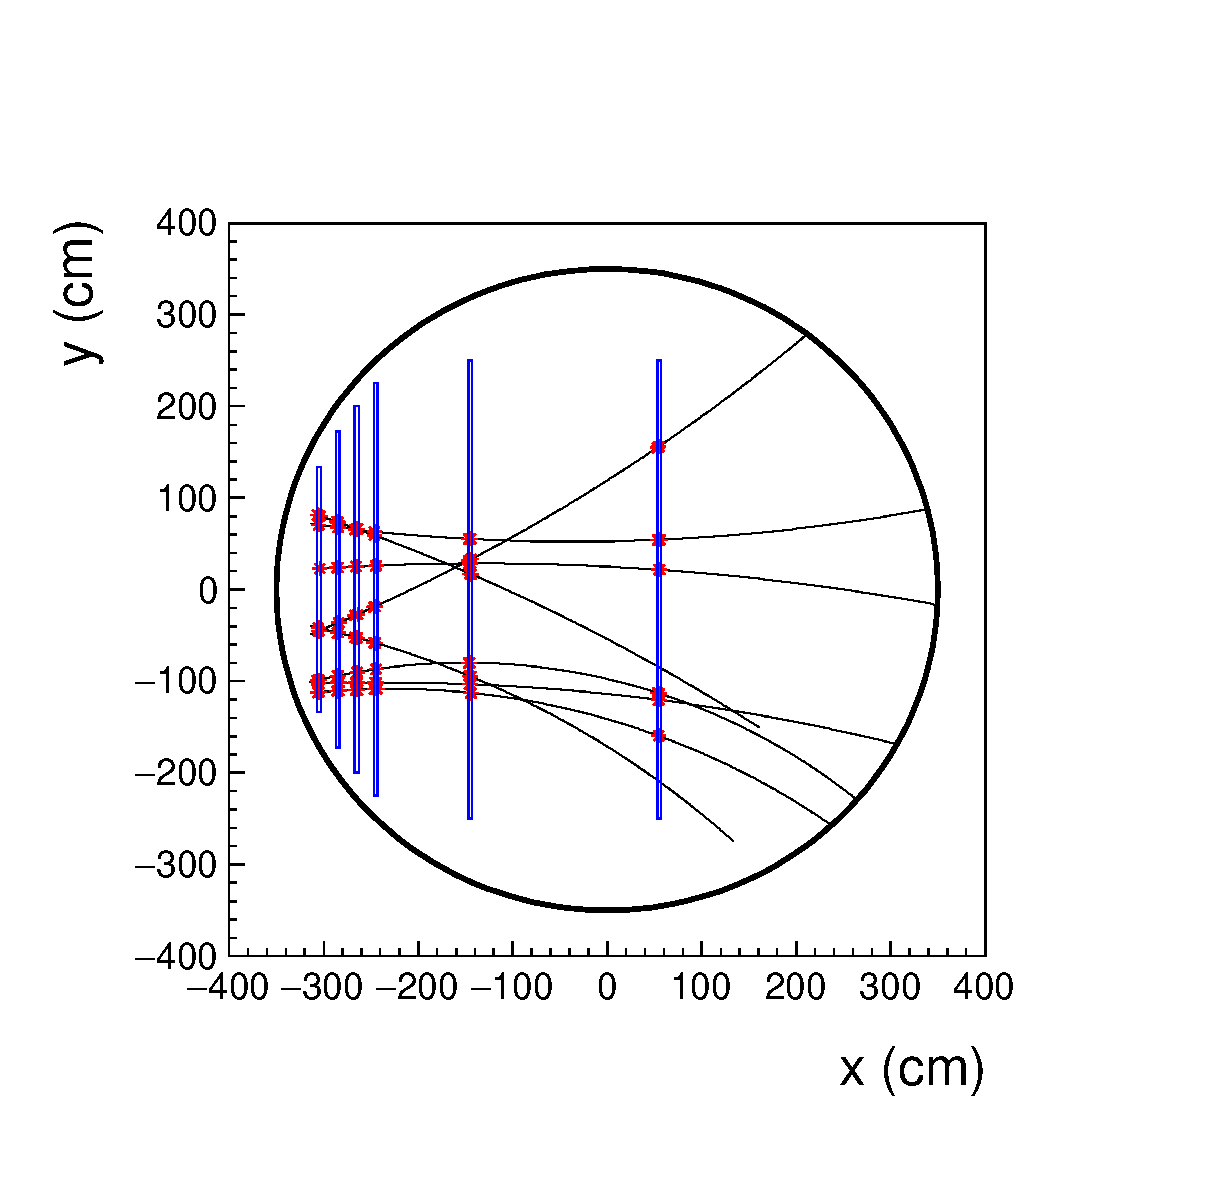
\includegraphics[width=\textwidth]{figures/ch4-KF_NDGArLite/Toy/XY_view.eps}
         \caption{}
         \label{fig:XYViewGArLite}
     \end{subfigure}
        \caption[Toy Monte Carlo event display for ND-GAr-Lite.]{Toy Monte Carlo event display showing 8 muon tracks from the simulated sample in (a) $zy$ and (b) $xy$ view. The edges of the cylindrical tracking region are outlined in black, while the tracking planes are outlined in blue. The simulated trajectories are traced in black, while the plane hits are highlighted with red markers.} \label{fig:ViewGArLite}
\end{figure}

The difference between the two samples stems from the reconstruction. In both cases the \texttt{Seed} algorithm followed by the KF algorithm are used sequentially, but only in the second case the Energy Loss and Multiple Scattering corrections are applied to both portions of the algorithm (i.e. the \texttt{Seed} algorithm and the KF). The purpose of comparing the two samples is to show the impact that the energy loss and multiple scattering corrections have on the reconstruction, as well as to verify that the simulation and reconstruction algorithms are internally consistent. We denote the sample in which the material budget corrections are not applied as the Non Corrected Sample or NC Sample and the other sample as the Corrected Sample or C Sample.

An example event display showing 8 muon tracks from the simulated sample are shown in in Fig. \ref{fig:ViewGArLite} both in a $zy$ and $xy$ view. The edges of the cylindrical tracking region are outlined in black, while the tracking planes are outlined in blue. The simulated trajectories are traced in black, while the plane hits are highlighted with red markers.

\begin{figure}[t]
     \centering
     \begin{subfigure}[b]{0.48\textwidth}
         \centering
         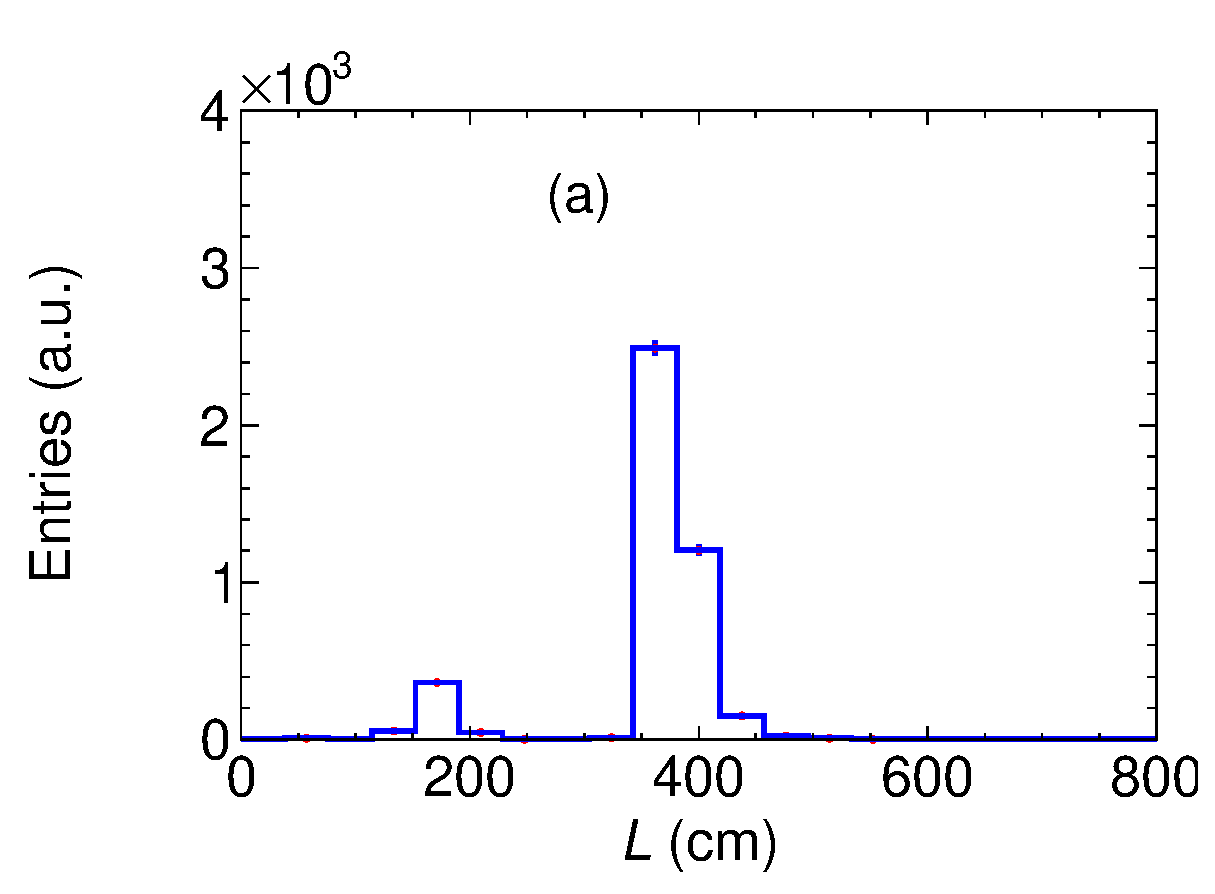
\includegraphics[width=\textwidth]{figures/ch4-KF_NDGArLite/Toy/LengthAllTall.eps}
         \caption{}
         \label{fig:ToyGArLite_L}
     \end{subfigure}
     \begin{subfigure}[b]{0.48\textwidth}
         \centering
         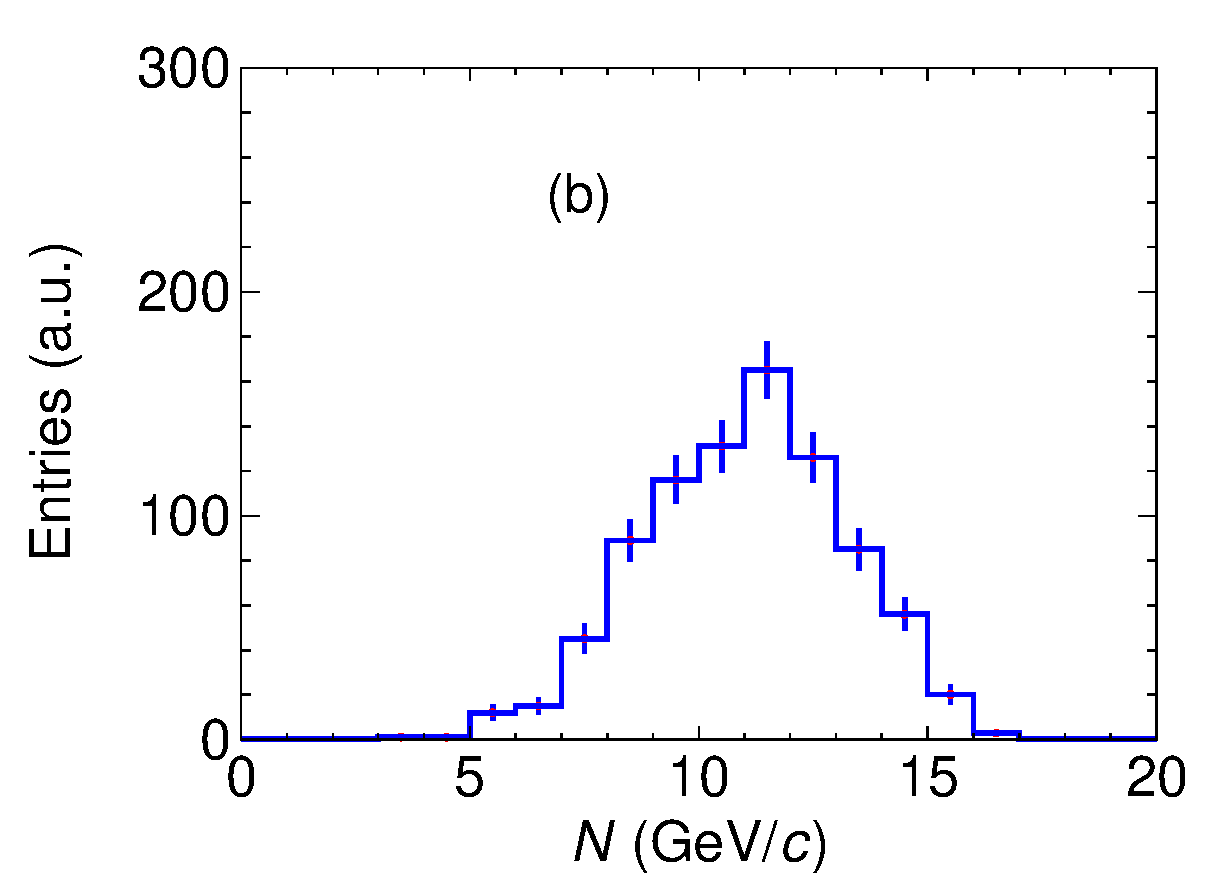
\includegraphics[width=\textwidth]{figures/ch4-KF_NDGArLite/Toy/NPointsAllTall.eps}
         \caption{}
         \label{fig:ToyGArLite_N}
     \end{subfigure}
          \begin{subfigure}[b]{0.48\textwidth}
         \centering
         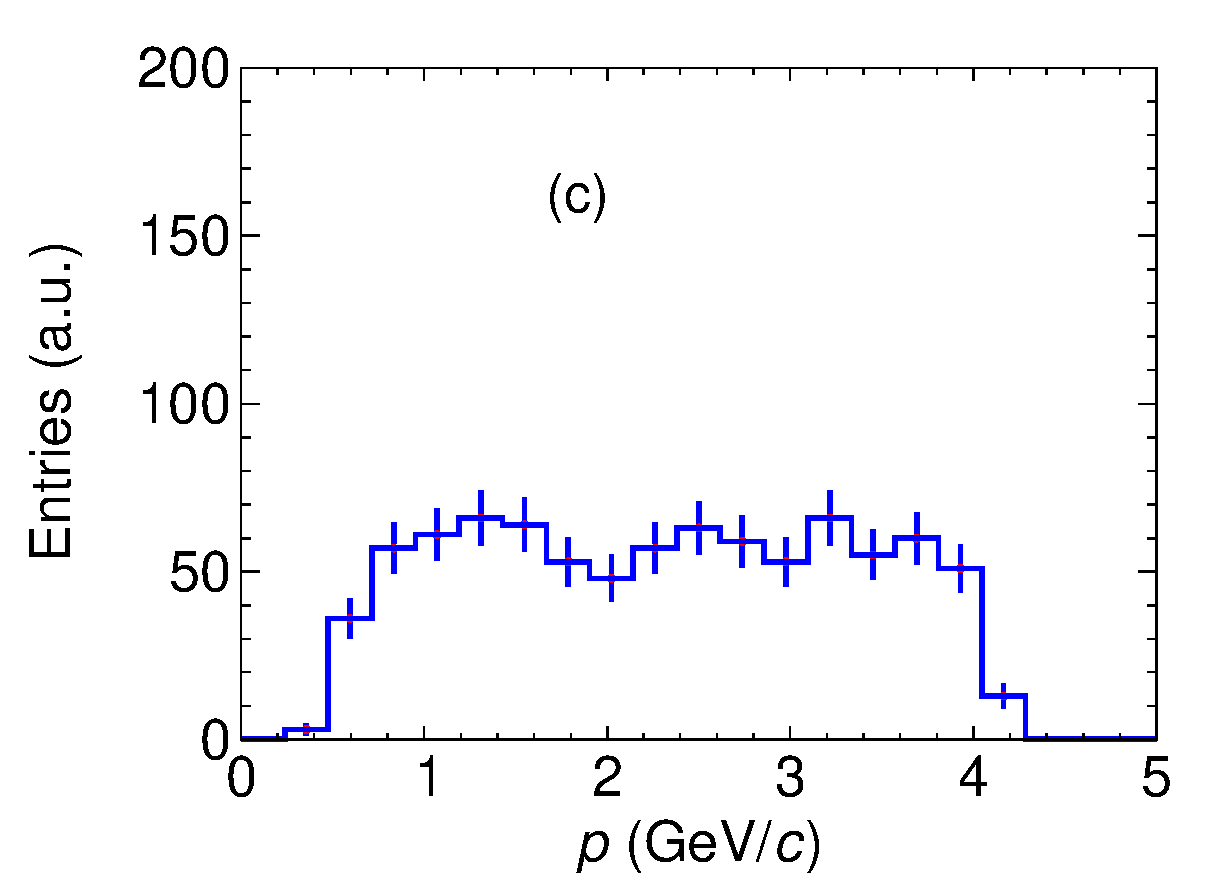
\includegraphics[width=\textwidth]{figures/ch4-KF_NDGArLite/Toy/pAllTall.eps}
         \caption{}
         \label{fig:ToyGArLite_p}
     \end{subfigure}
     \begin{subfigure}[b]{0.48\textwidth}
         \centering
         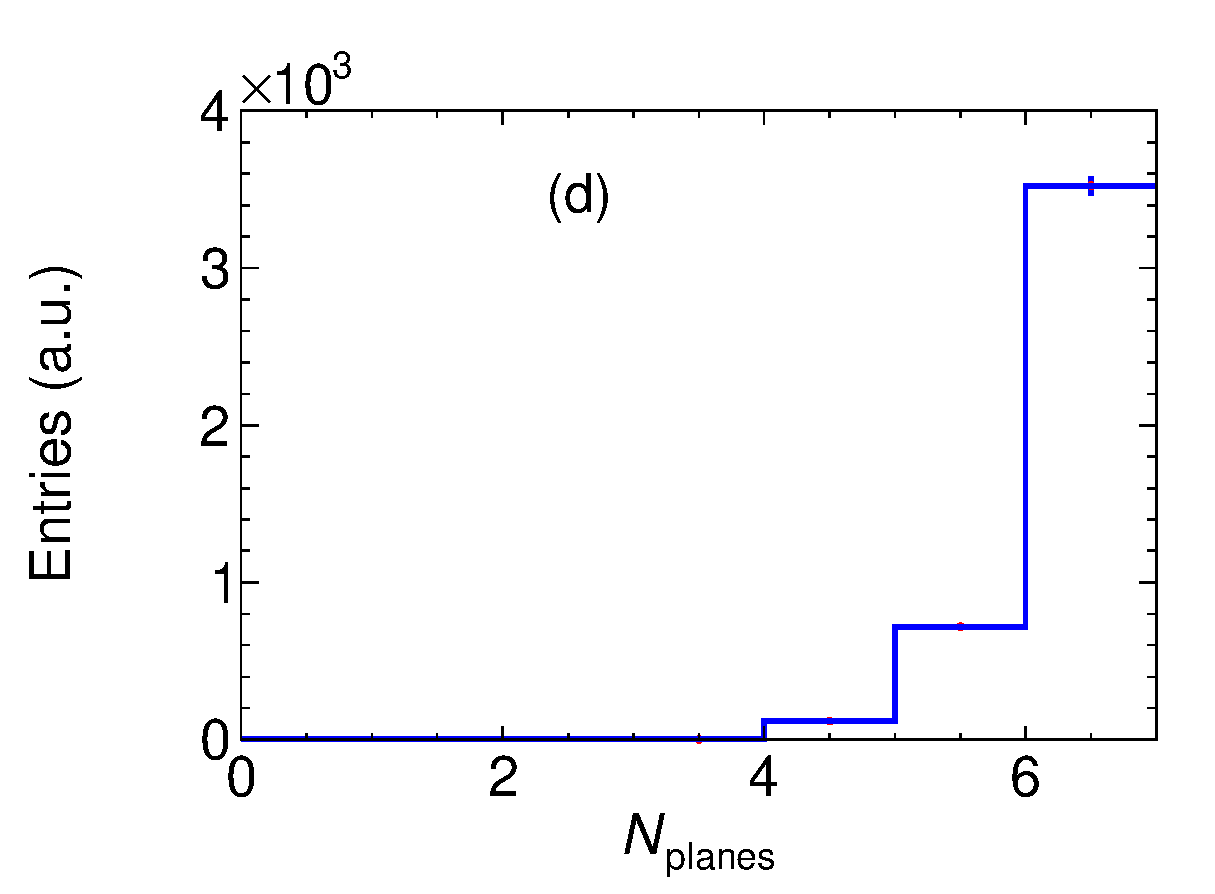
\includegraphics[width=\textwidth]{figures/ch4-KF_NDGArLite/Toy/NPlanesAllTall.eps}
         \caption{}
         \label{fig:ToyGArLite_planes}
     \end{subfigure}
        \caption[Properties of the particles simulated for the Toy Monte Carlo NC and C samples.]{Properties of the particles simulated for the Toy Monte Carlo NC and C samples: (a) length of the particle tracks $L$ (cm) measured as the summed distances between the hit clusters; (b) number of hit clusters belonging to the tracks $N$; (c) initial momentum of the particles $p$ (GeV/$c$); (d) total number of tracking planes traversed by the particle $N_\text{planes}.$} \label{fig:ToyGArLite_prop}
\end{figure}

\begin{figure}[t]
     \centering
     \begin{subfigure}{0.32\textwidth}
         \centering
         \includegraphics[width=\textwidth]{figures/ch4-KF_NDGArLite/Toy/NoCorr/UnitSeed_p0.eps}
         \caption{}
         \label{fig:resp0Seed_GArLite_NoCorr}
     \end{subfigure}
     \begin{subfigure}{0.32\textwidth}
         \centering
         \includegraphics[width=\textwidth]{figures/ch4-KF_NDGArLite/Toy/NoCorr/UnitSeed_p1.eps}
         \caption{}
         \label{fig:resp1Seed_GArLite_NoCorr}
     \end{subfigure}
    \begin{subfigure}{0.32\textwidth}
         \centering
         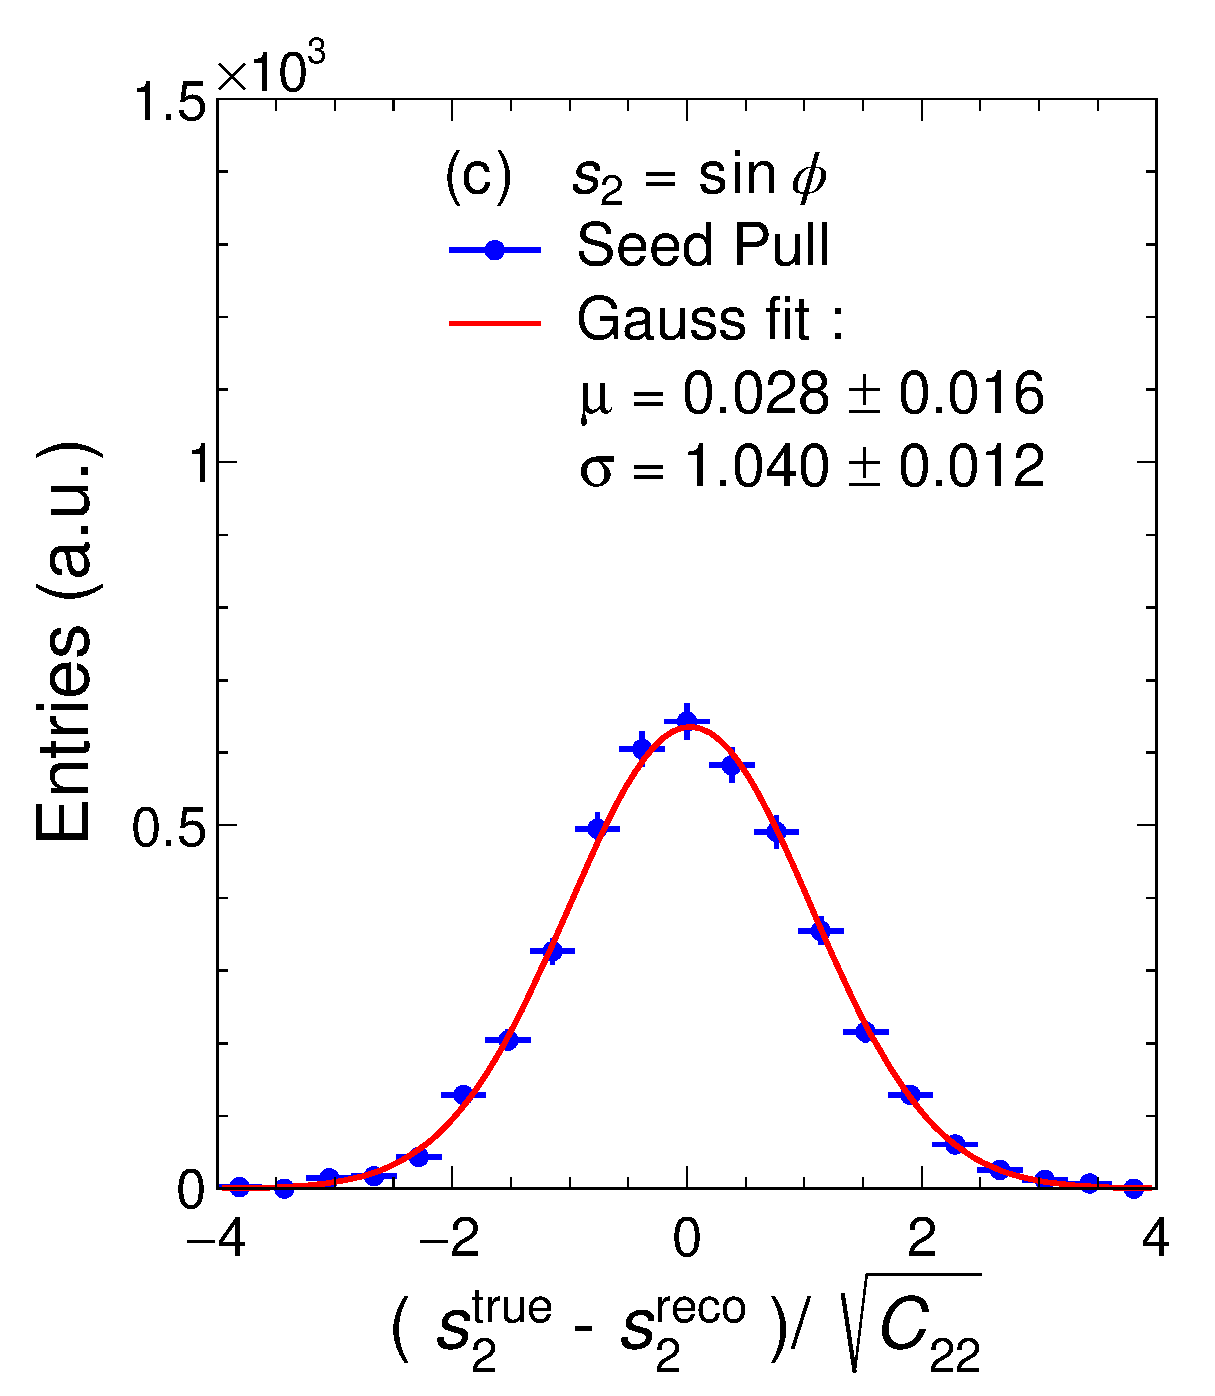
\includegraphics[width=\textwidth]{figures/ch4-KF_NDGArLite/Toy/NoCorr/UnitSeed_p2.eps}
         \caption{}
         \label{fig:resp2Seed_GArLite_NoCorr}
     \end{subfigure}
          \begin{subfigure}{0.32\textwidth}
         \centering
         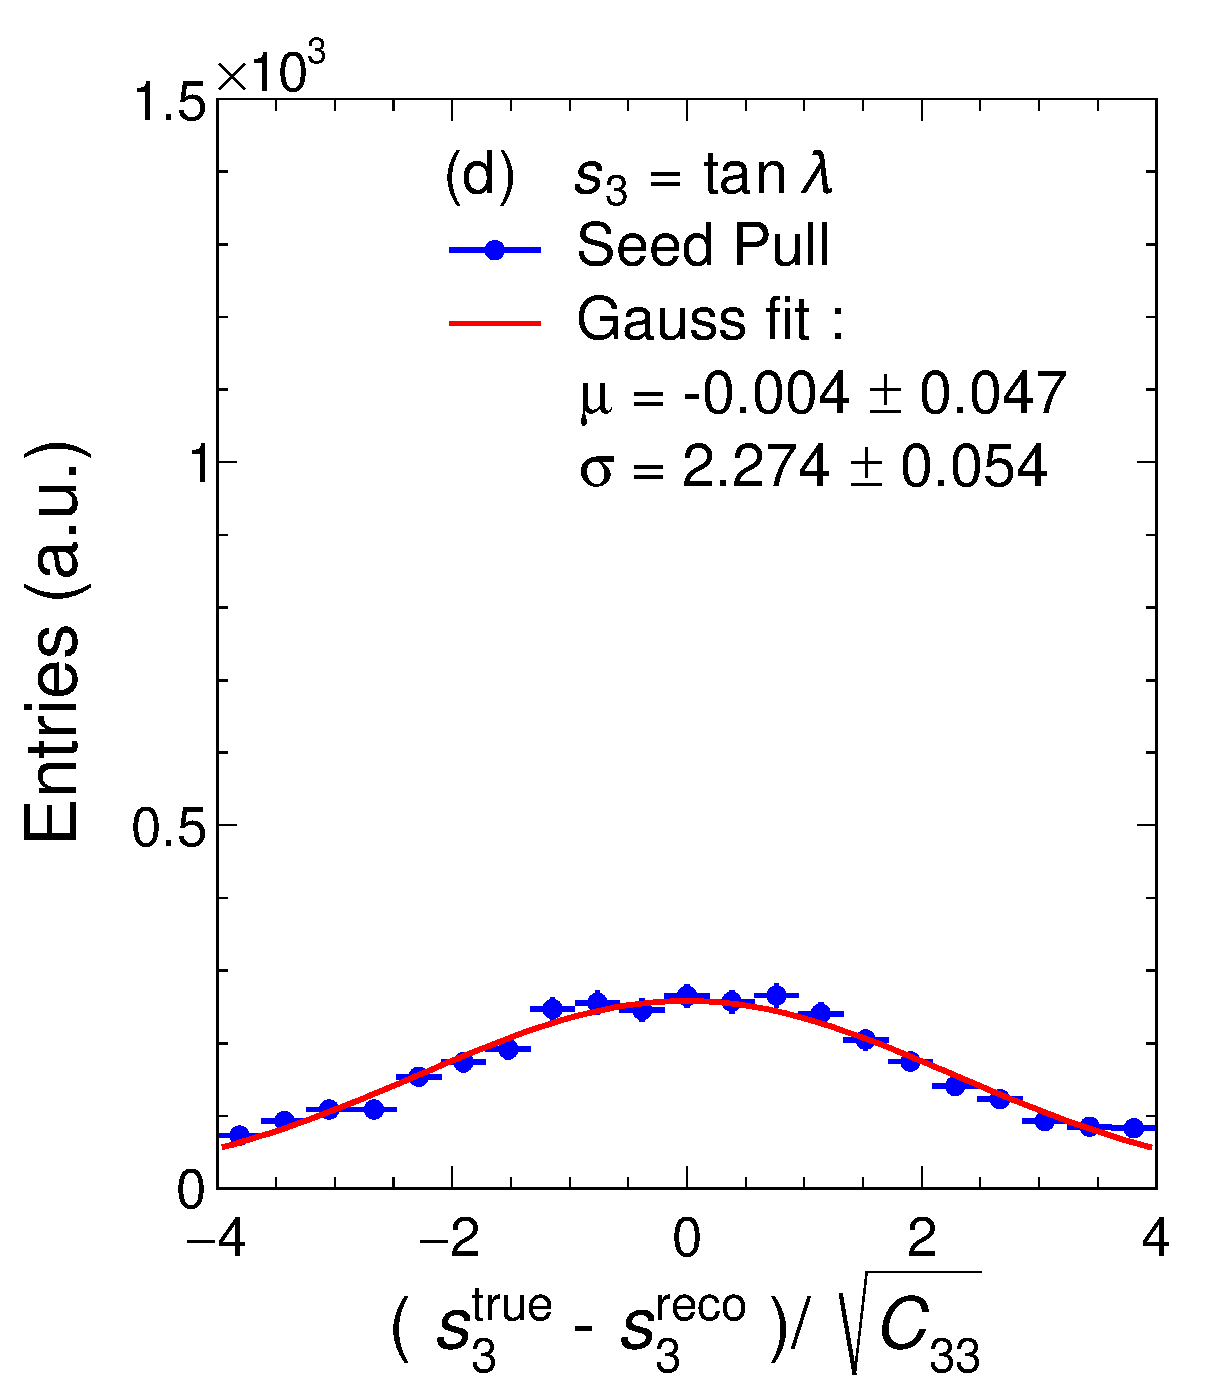
\includegraphics[width=\textwidth]{figures/ch4-KF_NDGArLite/Toy/NoCorr/UnitSeed_p3.eps}
         \caption{}
         \label{fig:resp3Seed_GArLite_NoCorr}
     \end{subfigure}
     \begin{subfigure}{0.32\textwidth}
         \centering
         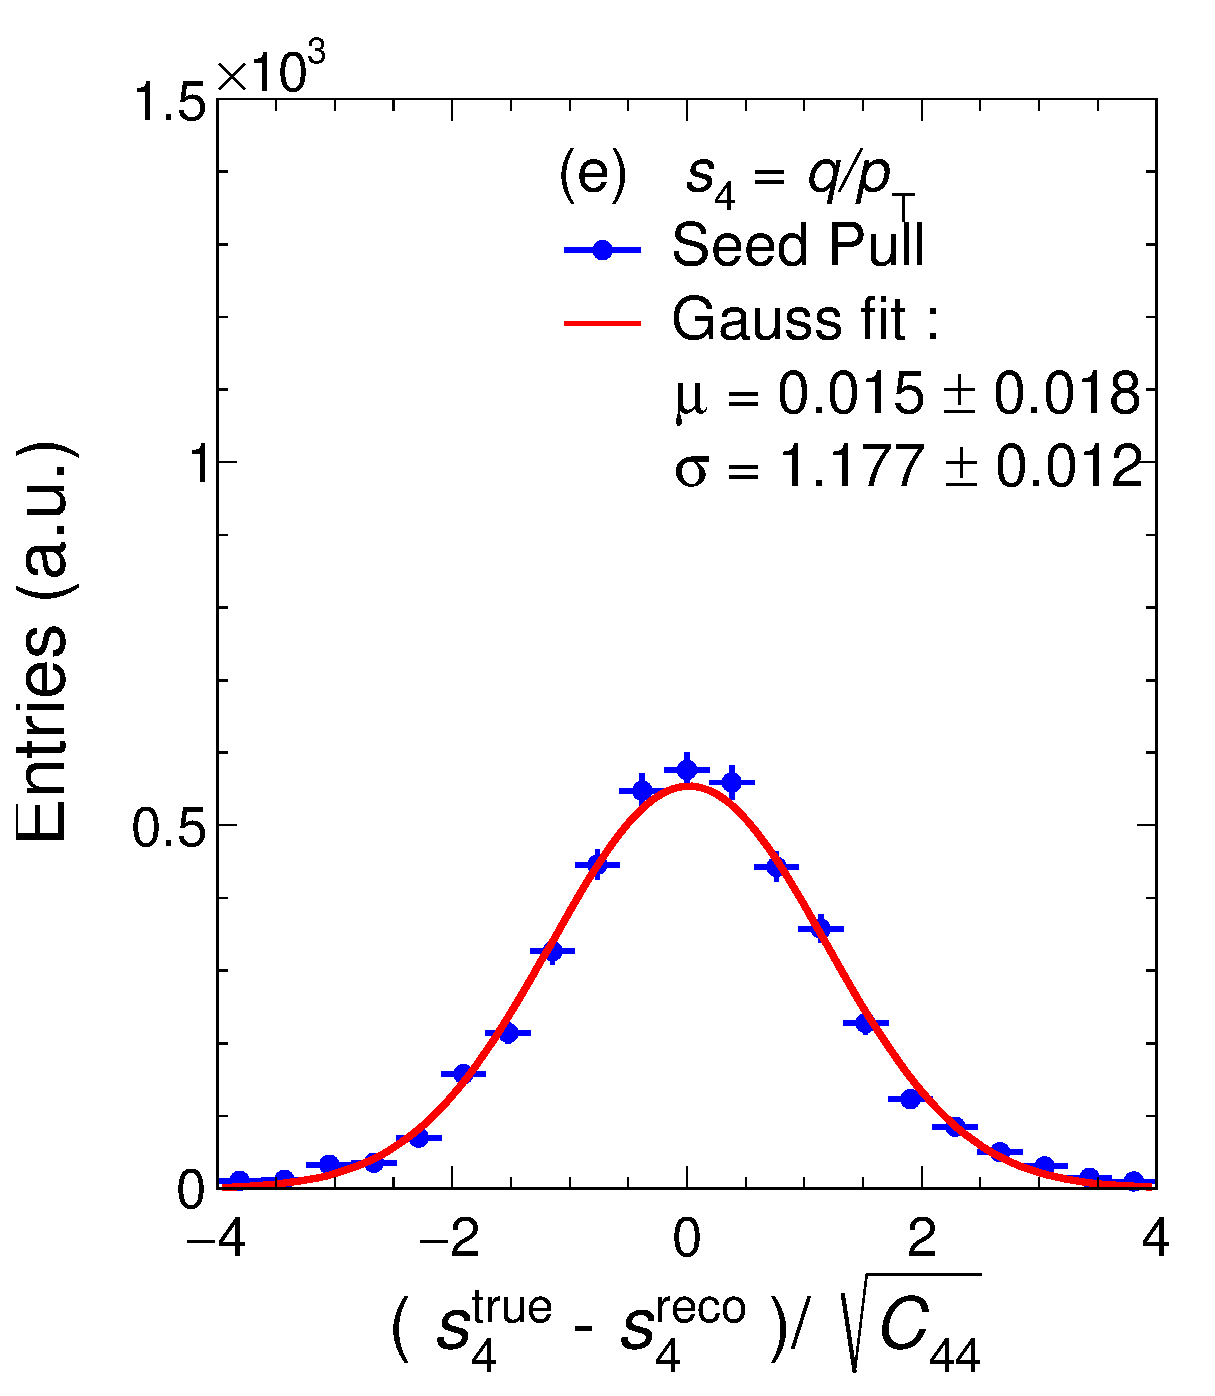
\includegraphics[width=\textwidth]{figures/ch4-KF_NDGArLite/Toy/NoCorr/UnitSeed_p4.eps}
         \caption{}
         \label{fig:resp4Seed_GArLite_NoCorr}
     \end{subfigure}
        \caption[Pull distributions for the \texttt{Seed} algorithm over the Non-Corrected sample.]{Pull distributions for the \texttt{Seed} algorithm over the Non-Corrected sample. All distributions were fitted to a Gaussian function. Results for parameters $s_0$ to $s_4$ (i.e. $y$, $x$, $\sin\phi$, $\tan\lambda$ and $q/p_{\text{T}}$) are shown from left to right and labeled from (a) to (e) accordingly. }
        \label{fig:ToyUnitSeed_GArLite_NoCorr}
\end{figure}

Some key quantities that describe the properties of the two samples are shown in Fig. \ref{fig:ToyGArLite_prop}. Fig. \ref{fig:ToyGArLite_L} shows the distribution of the tracks lengths $L$ in cm's defined as the total distance between the scintillator planes hit clusters. The distribution shows two clear peaks: one between 100 and 200 cm's and the other around 400cm. The two-peak distribution is easily explained by considering the disposition of the tracking planes in the 6-plane geometry for ND-GAr-Lite. In the 6-planes geometry the first 5 planes are disposed within the first 200 cm of the detector cylinder in the beam direction, while the last one is set 200 cm apart from all the others. This is confirmed by Fig. \ref{fig:ToyGArLite_planes} which shows the number of plains which are traversed by each particle in the samples. Most tracks in the samples cross the whole 6 planes and some cross either 4 or 5, explaining the two peaks in the $L$ distribution. Additionally Fig \ref{fig:ToyGArLite_N} shows the number of hit clusters $N$ associated with each track and Fig. \ref{fig:ToyGArLite_p} the initial true momentum $p$ of the particles.


\begin{figure}[t]
     \centering
     \begin{subfigure}{0.32\textwidth}
         \centering
         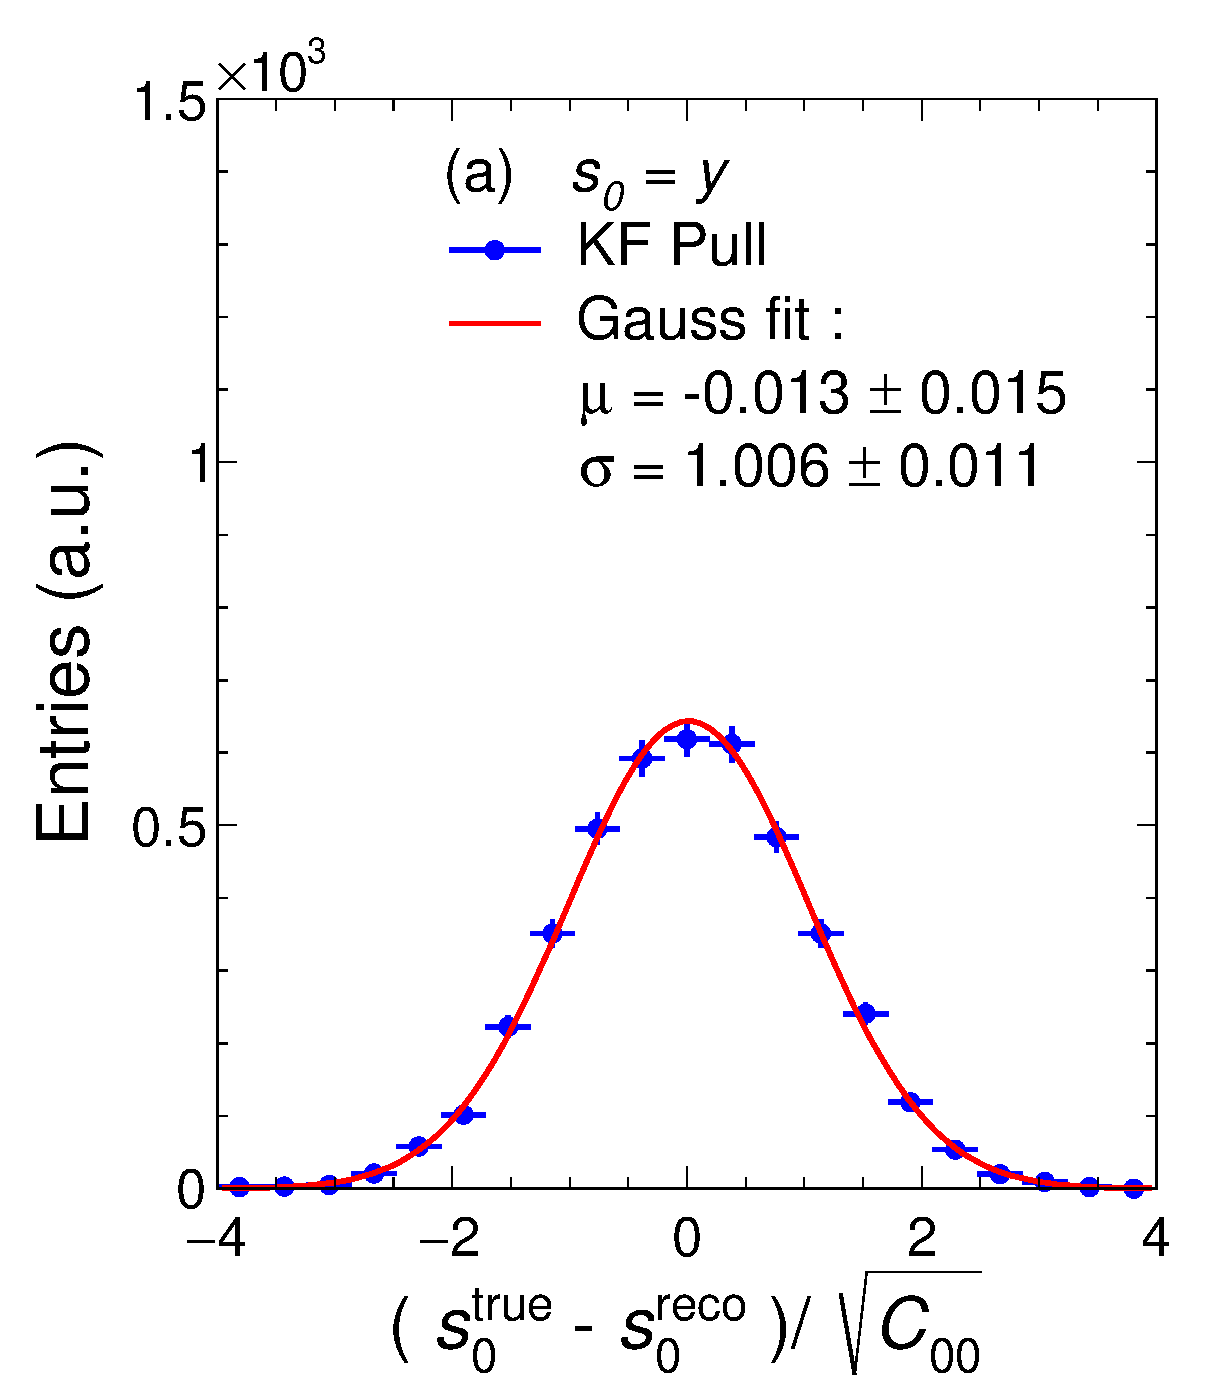
\includegraphics[width=\textwidth]{figures/ch4-KF_NDGArLite/Toy/NoCorr/UnitKFEnd_p0.eps}
         \caption{}
         \label{fig:resp0KF_GArLite_NoCorr}
     \end{subfigure}
     \begin{subfigure}{0.32\textwidth}
         \centering
         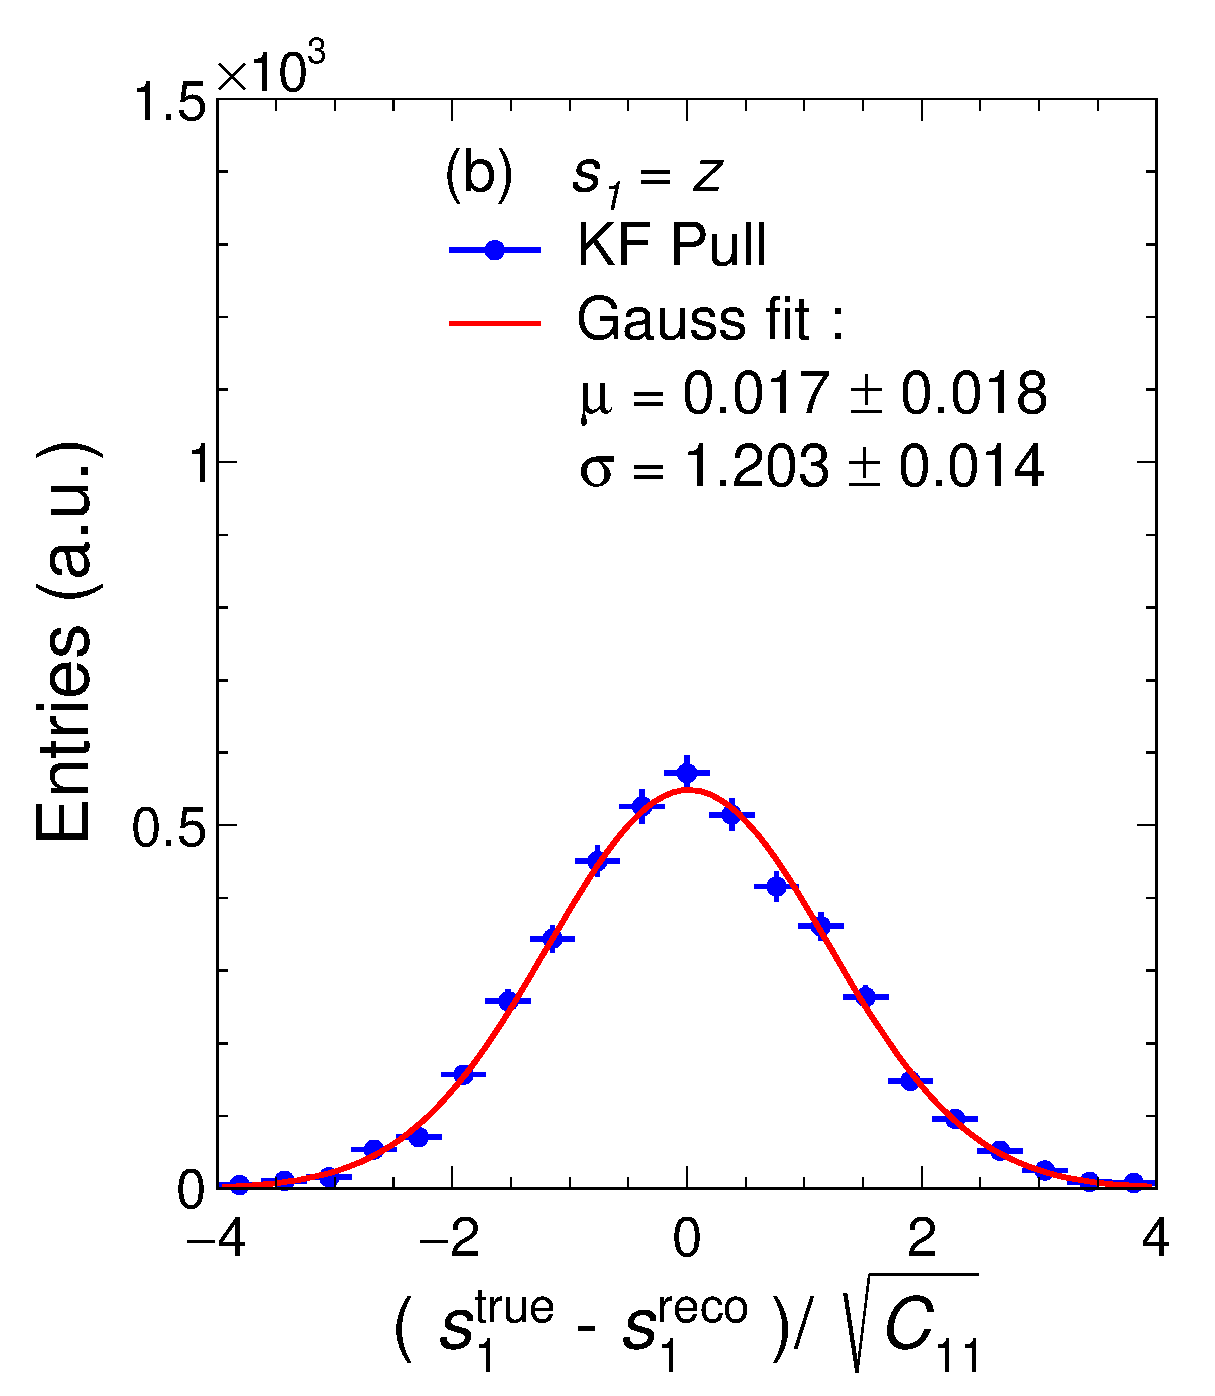
\includegraphics[width=\textwidth]{figures/ch4-KF_NDGArLite/Toy/NoCorr/UnitKFEnd_p1.eps}
         \caption{}
         \label{fig:resp1KF_GArLite_NoCorr}
     \end{subfigure}
    \begin{subfigure}{0.32\textwidth}
         \centering
         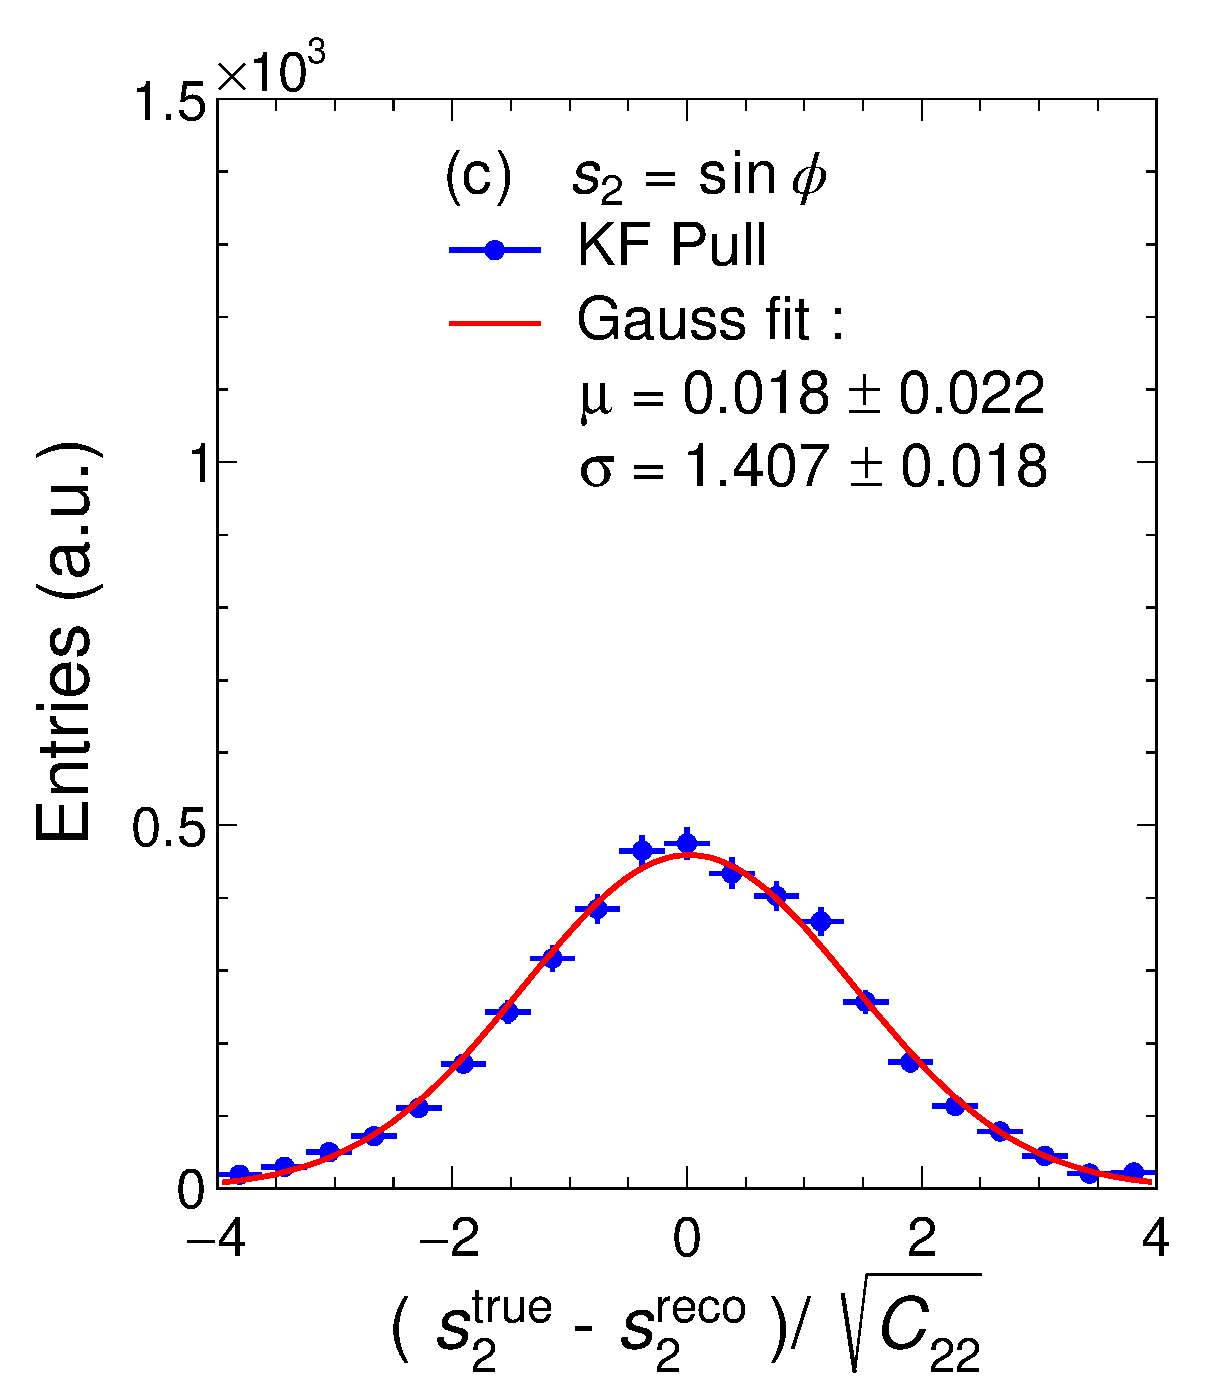
\includegraphics[width=\textwidth]{figures/ch4-KF_NDGArLite/Toy/NoCorr/UnitKFEnd_p2.eps}
         \caption{}
         \label{fig:resp2KF_GArLite_NoCorr}
     \end{subfigure}
          \begin{subfigure}{0.32\textwidth}
         \centering
         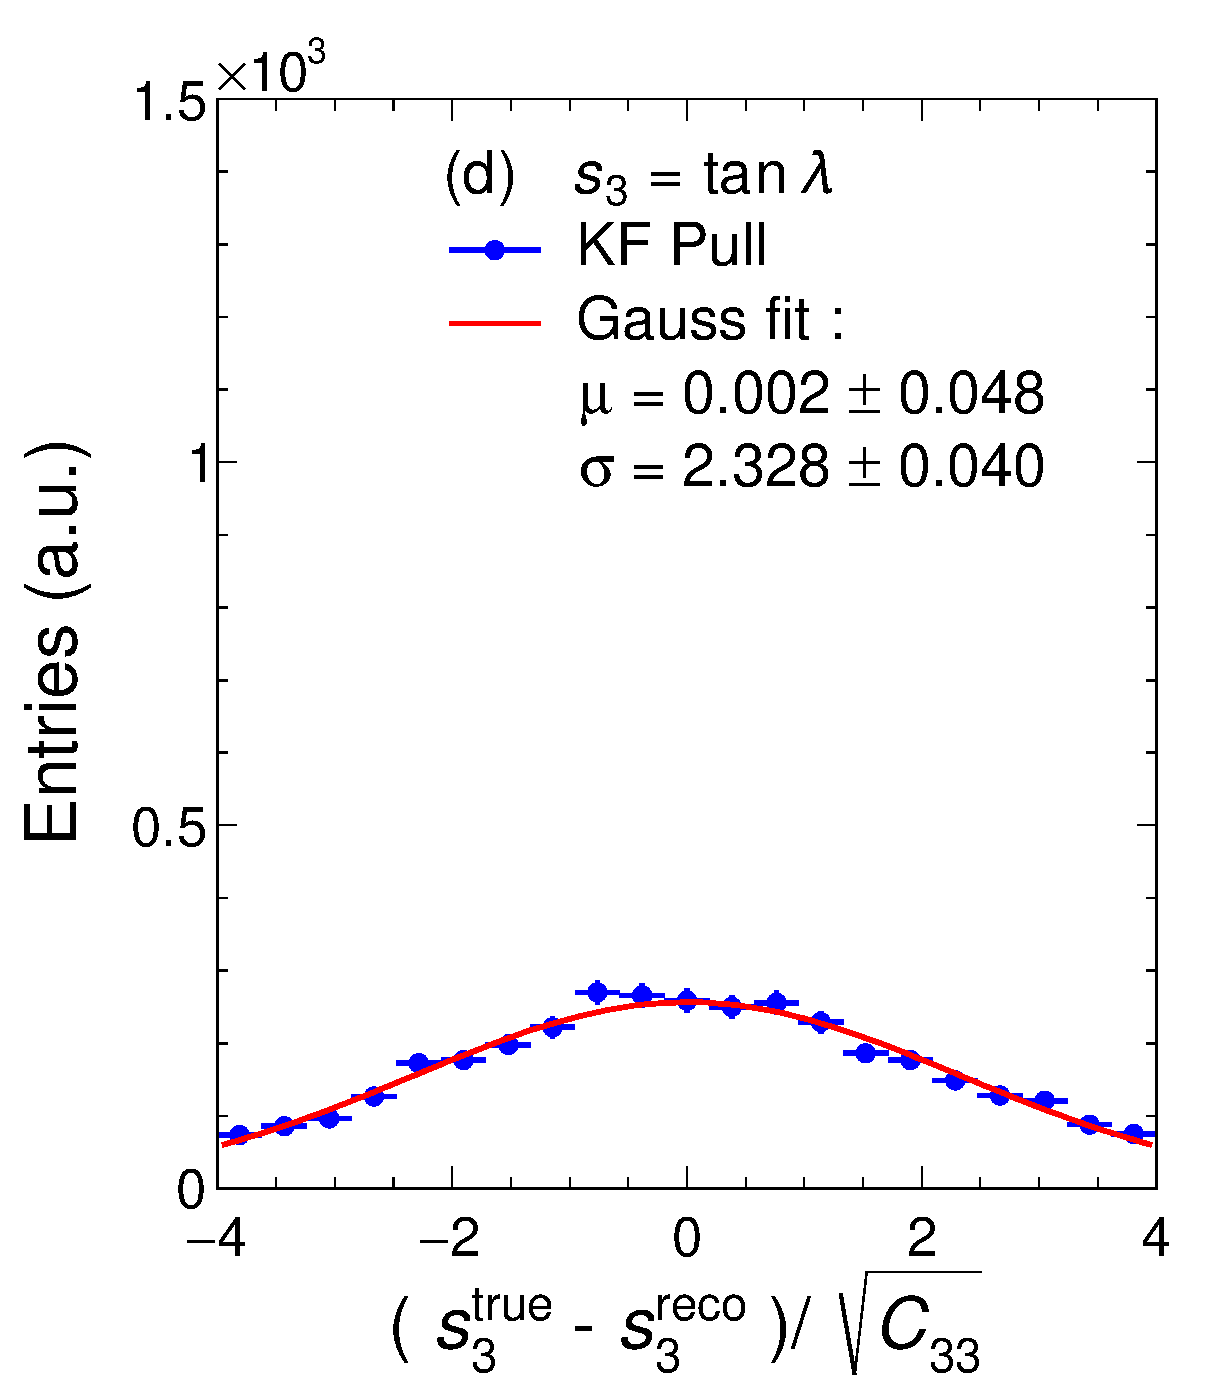
\includegraphics[width=\textwidth]{figures/ch4-KF_NDGArLite/Toy/NoCorr/UnitKFEnd_p3.eps}
         \caption{}
         \label{fig:resp3KF_GArLite_NoCorr}
     \end{subfigure}
     \begin{subfigure}{0.32\textwidth}
         \centering
         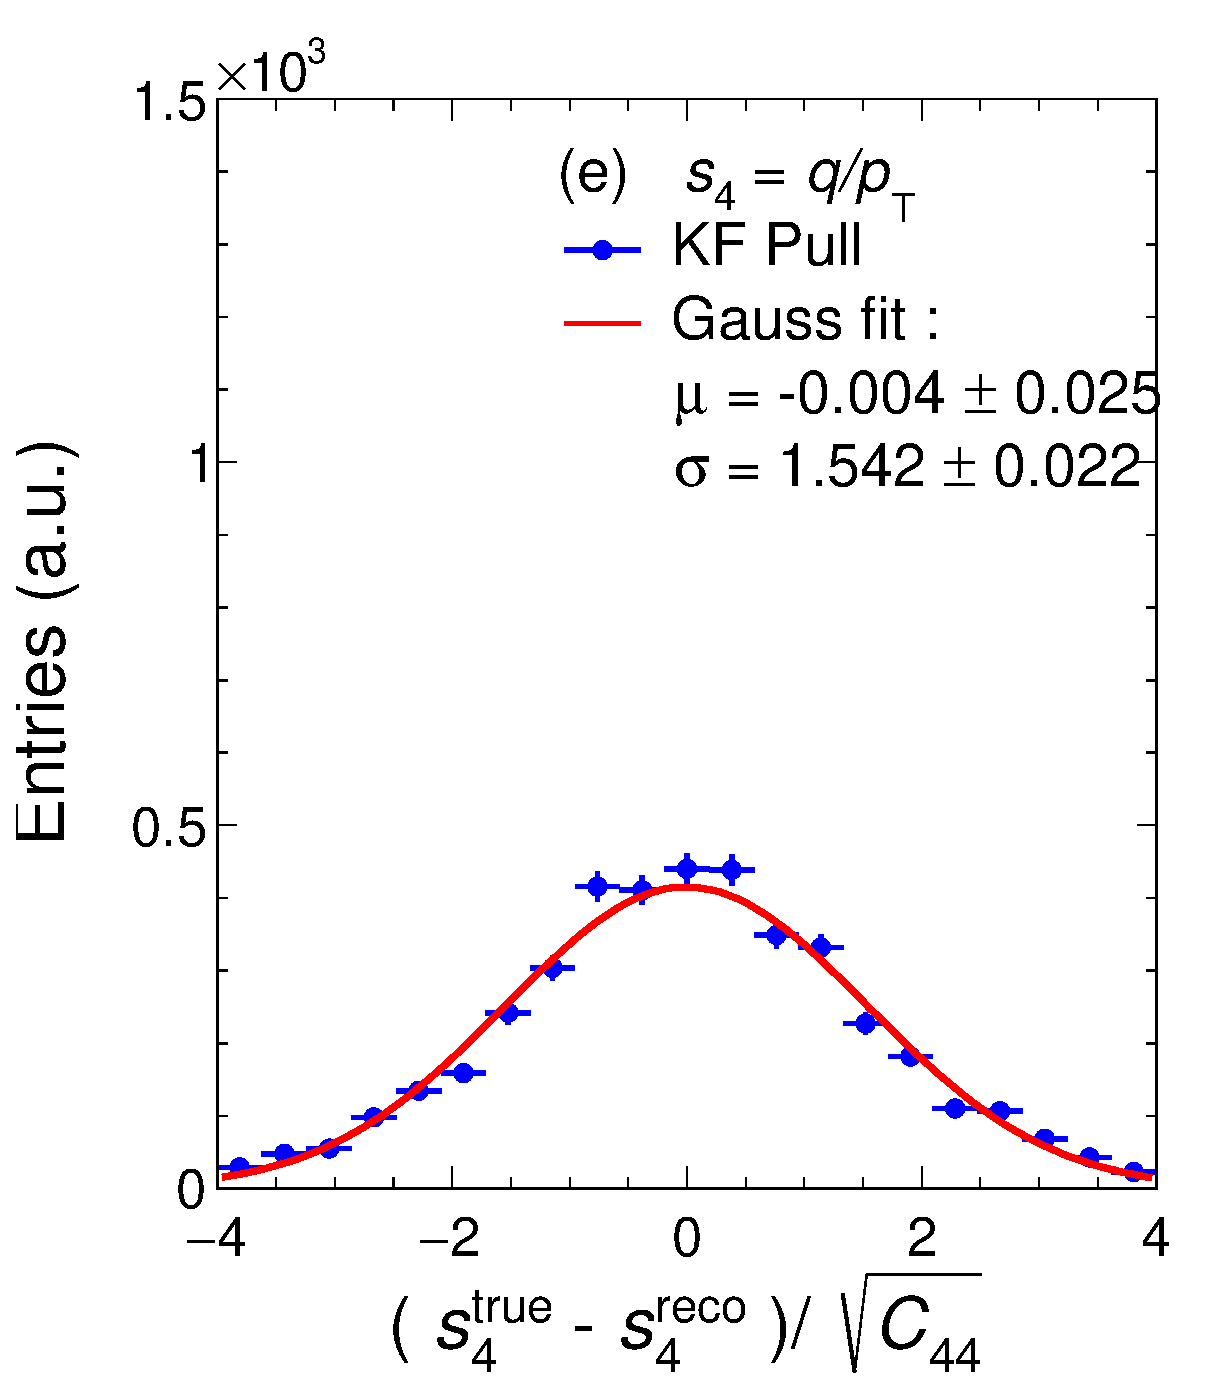
\includegraphics[width=\textwidth]{figures/ch4-KF_NDGArLite/Toy/NoCorr/UnitKFEnd_p4.eps}
         \caption{}
         \label{fig:resp4KF_GArLite_NoCorr}
     \end{subfigure}
        \caption[Pull distributions for the \texttt{KF-Lite} algorithm over the Non-Corrected (NC) sample.]{Pull distributions for the \texttt{KF-Lite} algorithm over the Non-Corrected (NC) sample. All distributions were fitted to a Gaussian function. Results for parameters $s_0$ to $s_4$ (i.e. $y$, $x$, $\sin\phi$, $\tan\lambda$ and $q/p_{\text{T}}$) are shown from left to right and labeled from (a) to (e) accordingly. }
        \label{fig:ToyUnitKF_GArLite_NoCorr}
\end{figure}

\begin{figure}[t]
     \centering
     \begin{subfigure}{0.32\textwidth}
         \centering
         \includegraphics[width=\textwidth]{figures/ch4-KF_NDGArLite/Toy/Corr/UnitSeed_p0.eps}
         \caption{}
         \label{fig:resp0Seed_GArLite_Corr}
     \end{subfigure}
     \begin{subfigure}{0.32\textwidth}
         \centering
         \includegraphics[width=\textwidth]{figures/ch4-KF_NDGArLite/Toy/Corr/UnitSeed_p1.eps}
         \caption{}
         \label{fig:resp1Seed_GArLite_Corr}
     \end{subfigure}
    \begin{subfigure}{0.32\textwidth}
         \centering
         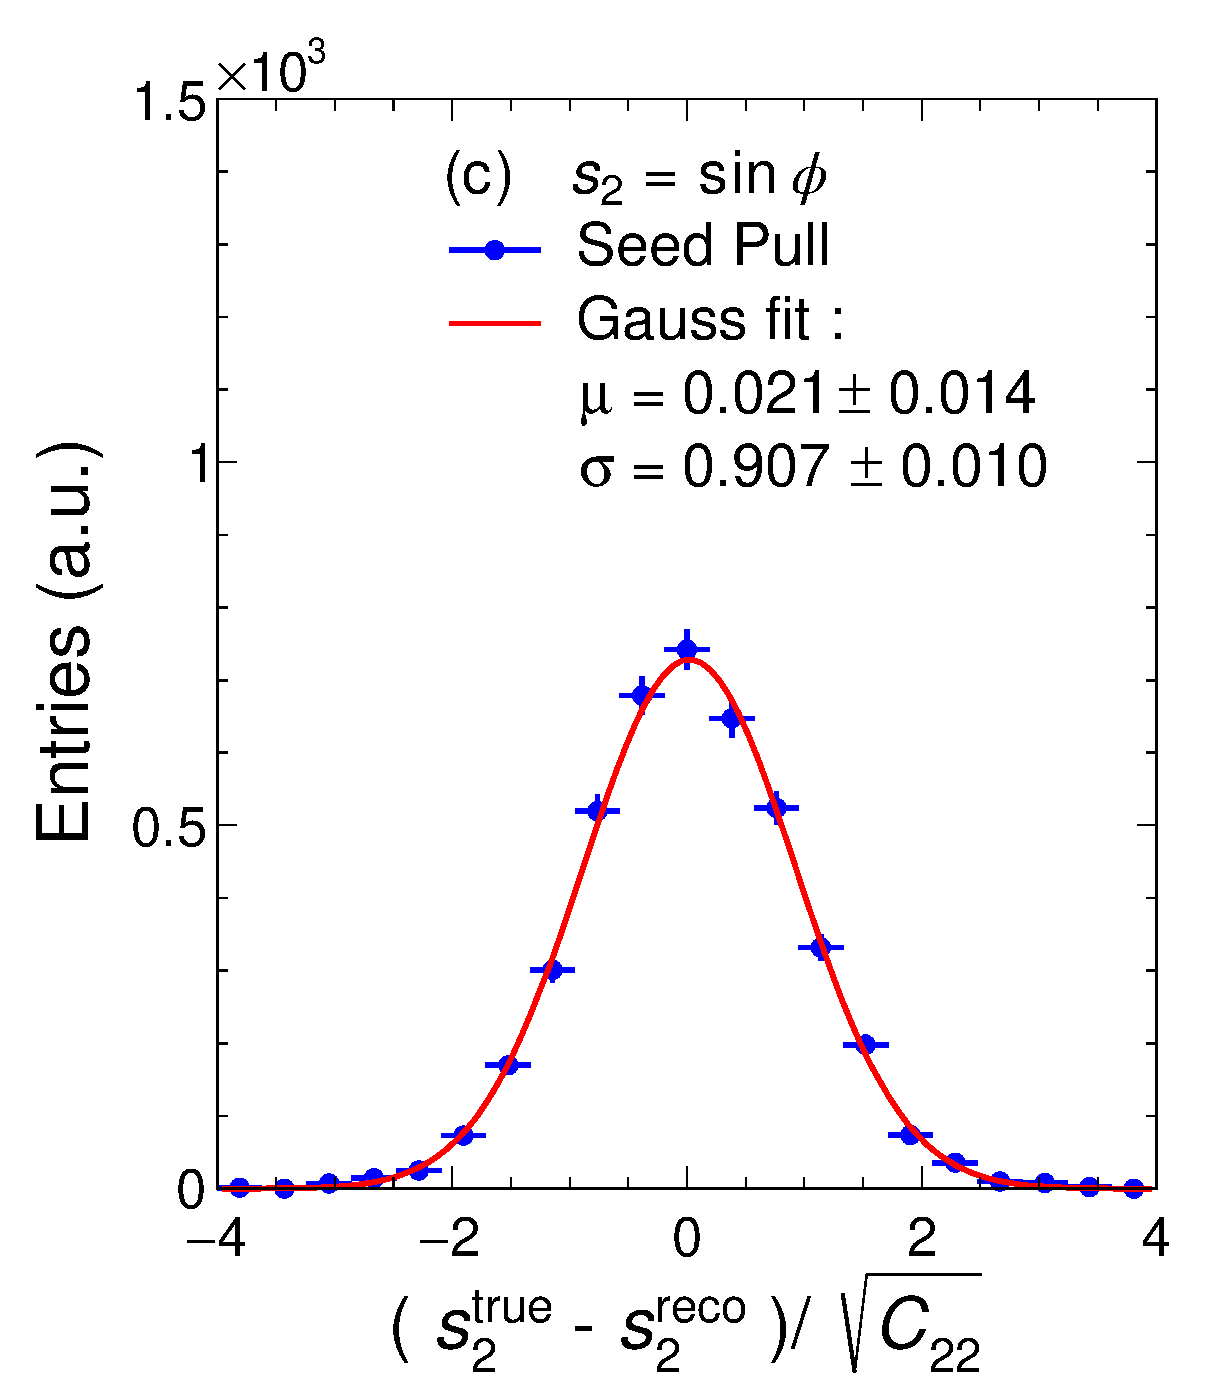
\includegraphics[width=\textwidth]{figures/ch4-KF_NDGArLite/Toy/Corr/UnitSeed_p2.eps}
         \caption{}
         \label{fig:resp2Seed_GArLite_Corr}
     \end{subfigure}
          \begin{subfigure}{0.32\textwidth}
         \centering
         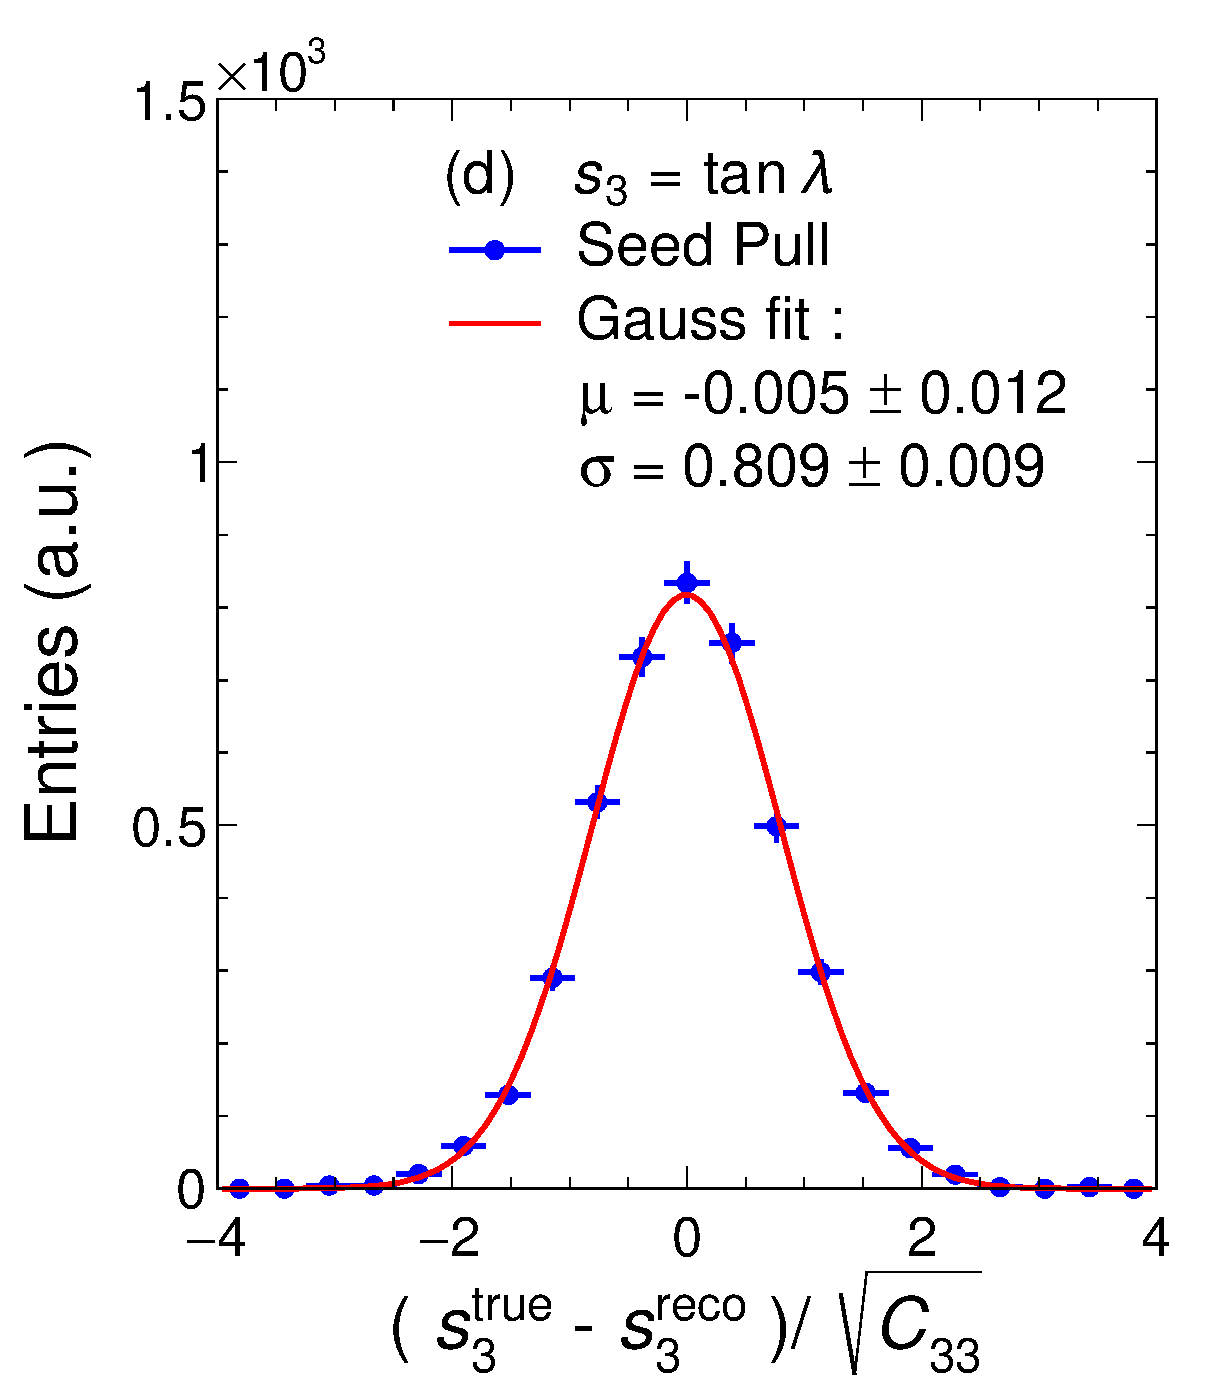
\includegraphics[width=\textwidth]{figures/ch4-KF_NDGArLite/Toy/Corr/UnitSeed_p3.eps}
         \caption{}
         \label{fig:resp3Seed_GArLite_Corr}
     \end{subfigure}
     \begin{subfigure}{0.32\textwidth}
         \centering
         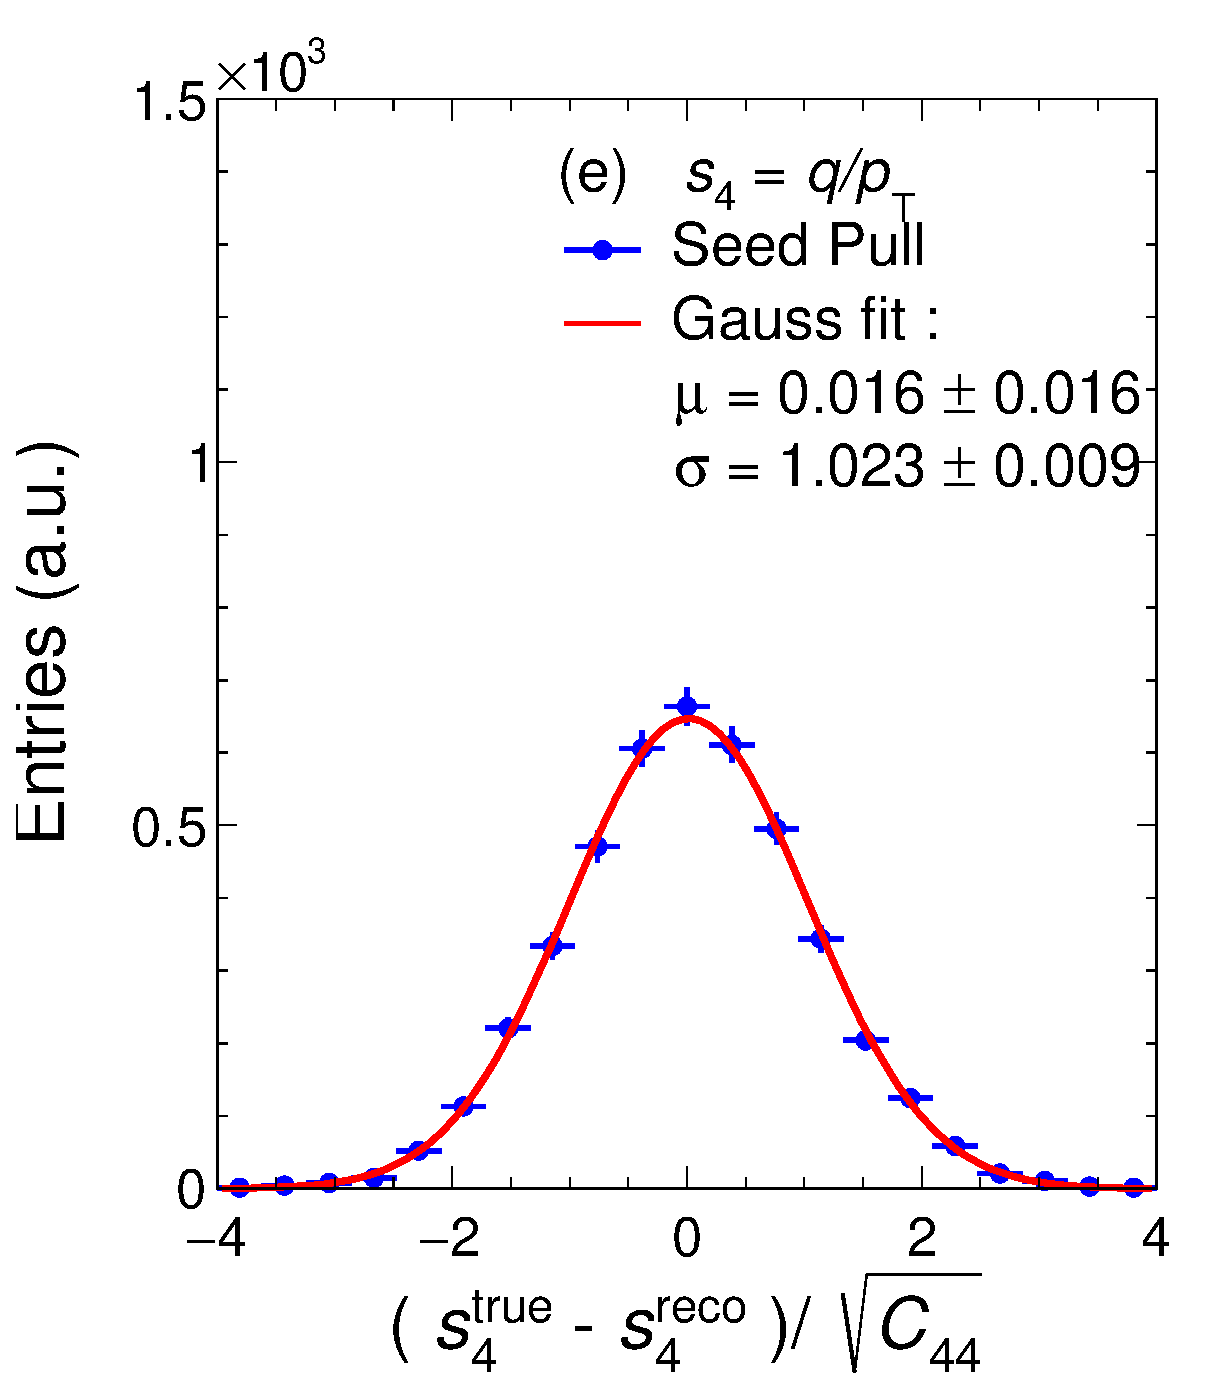
\includegraphics[width=\textwidth]{figures/ch4-KF_NDGArLite/Toy/Corr/UnitSeed_p4.eps}
         \caption{}
         \label{fig:resp4Seed_GArLite_Corr}
     \end{subfigure}
        \caption[Pull distributions for the \texttt{Seed} algorithm over the Corrected (C) sample.]{Pull distributions for the \texttt{Seed} algorithm over the Corrected (C) sample. All distributions were fitted to a Gaussian function. Results for parameters $s_0$ to $s_4$ (i.e. $y$, $x$, $\sin\phi$, $\tan\lambda$ and $q/p_{\text{T}}$) are shown from left to right and labeled from (a) to (e) accordingly. }
        \label{fig:ToyUnitSeed_GArLite_Corr}
\end{figure}

\begin{figure}[t]
     \centering
     \begin{subfigure}{0.32\textwidth}
         \centering
         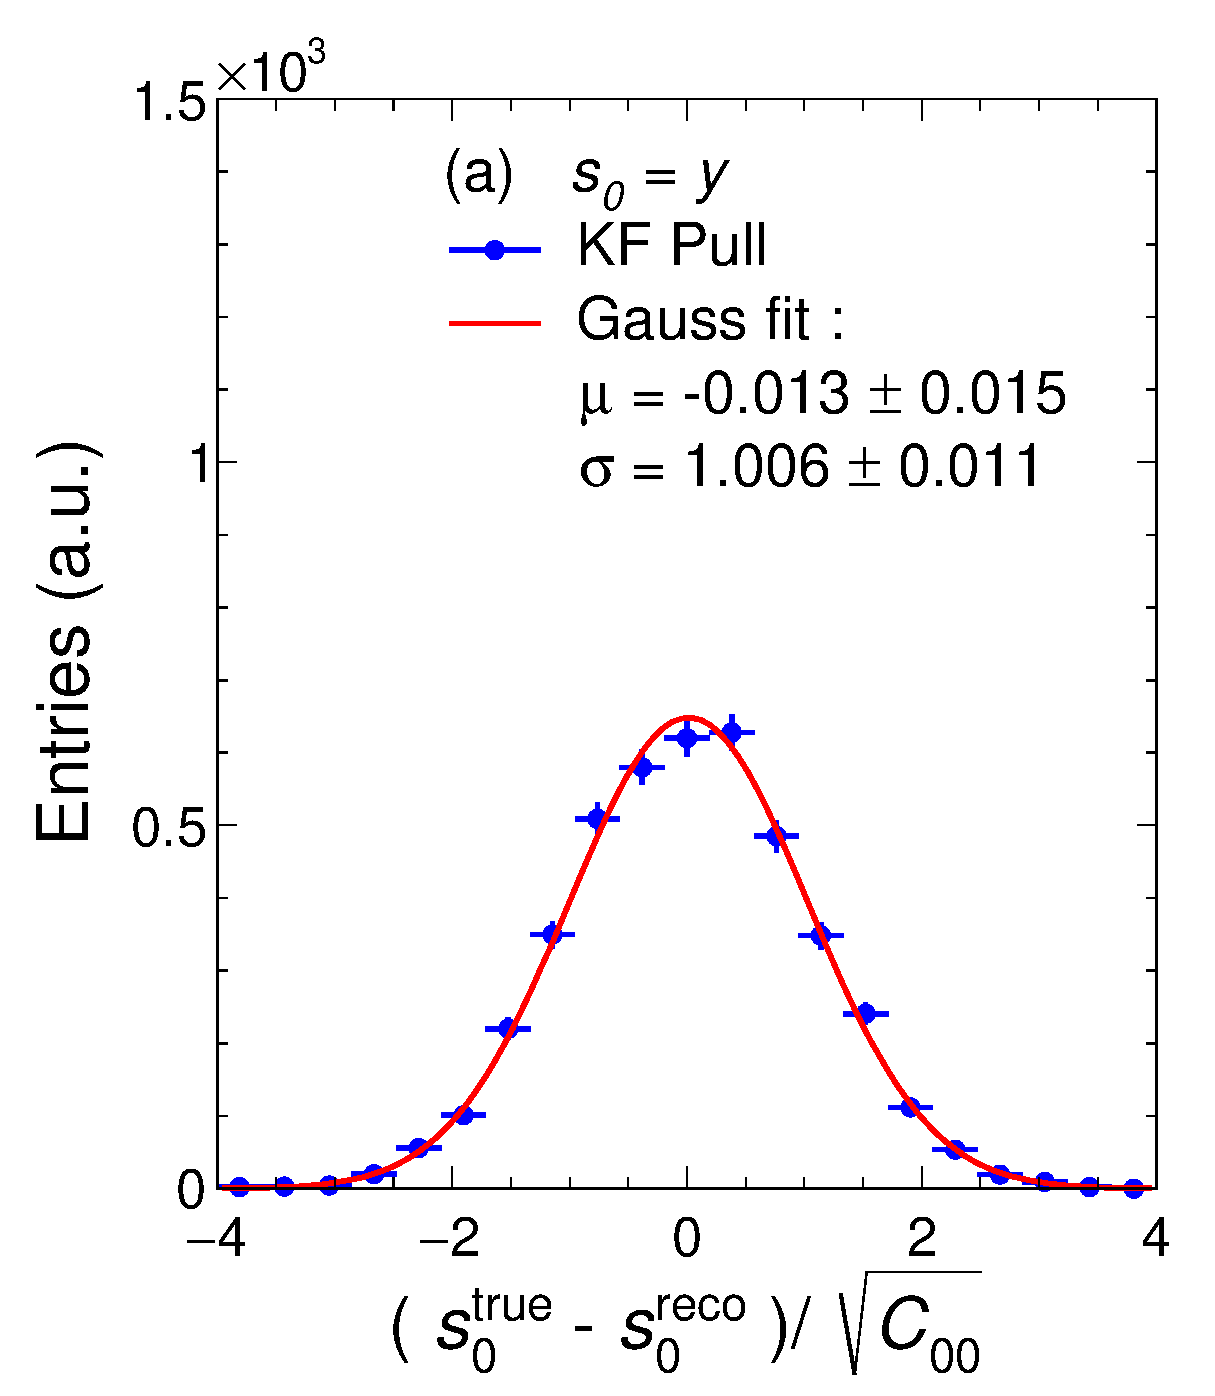
\includegraphics[width=\textwidth]{figures/ch4-KF_NDGArLite/Toy/Corr/UnitKFEnd_p0.eps}
         \caption{}
         \label{fig:resp0KF_GArLite_Corr}
     \end{subfigure}
     \begin{subfigure}{0.32\textwidth}
         \centering
         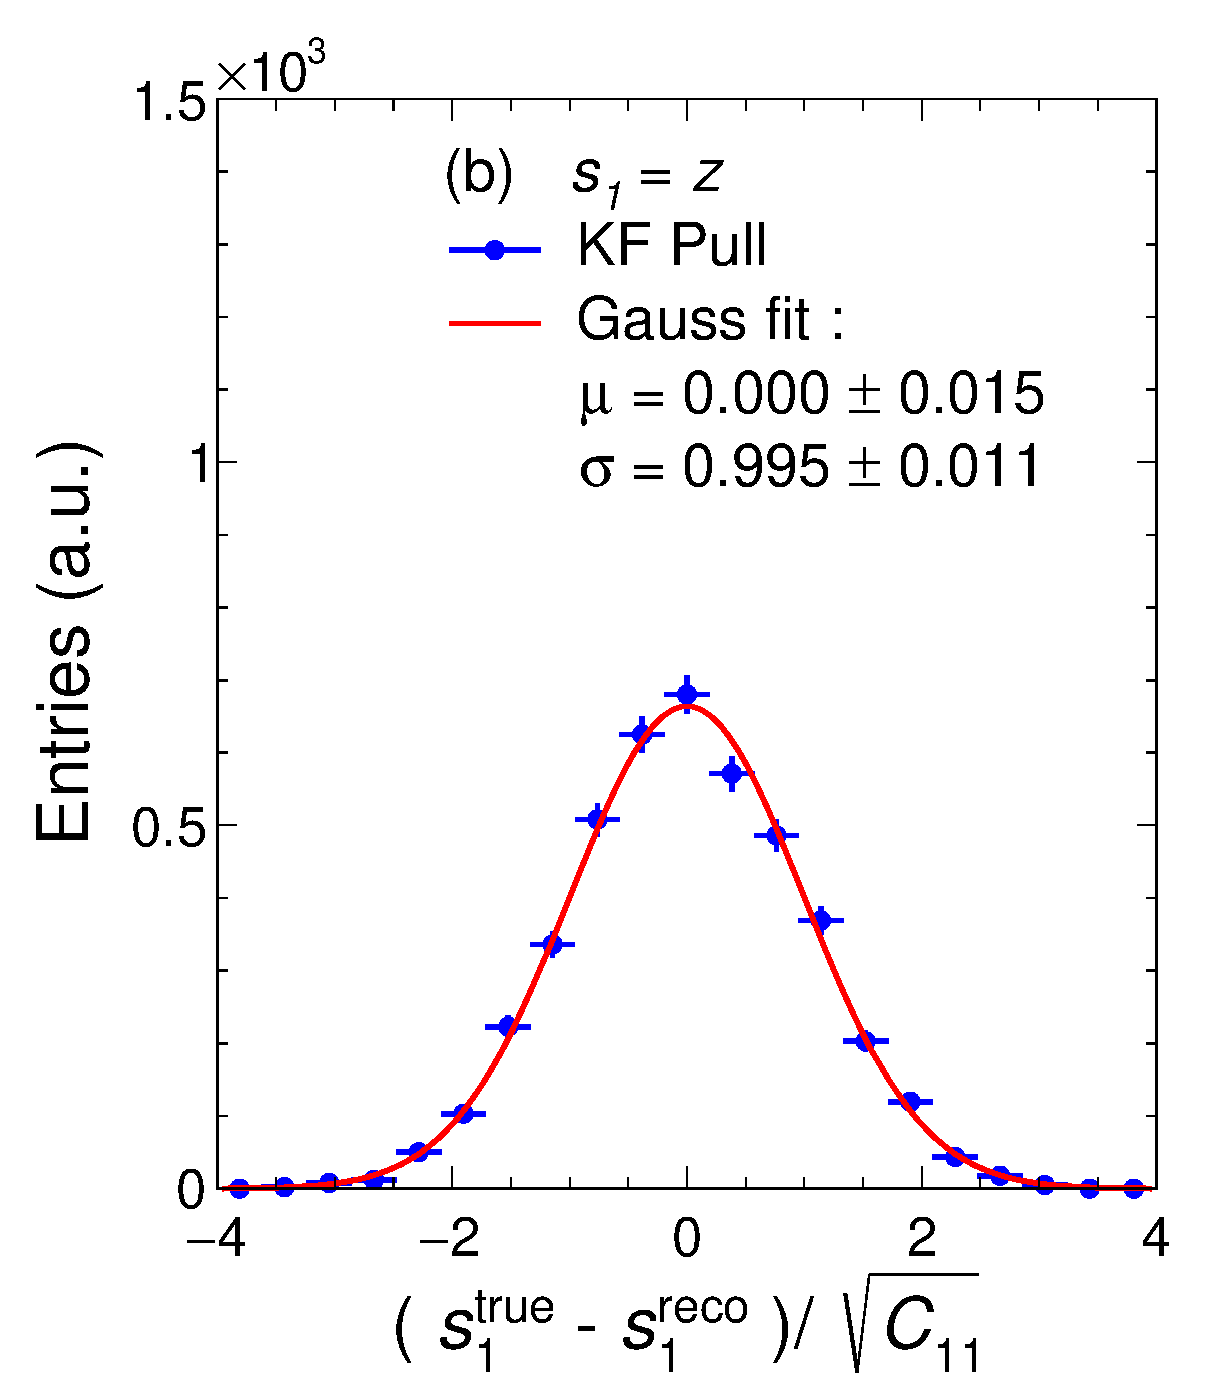
\includegraphics[width=\textwidth]{figures/ch4-KF_NDGArLite/Toy/Corr/UnitKFEnd_p1.eps}
         \caption{}
         \label{fig:resp1KF_GArLite_Corr}
     \end{subfigure}
    \begin{subfigure}{0.32\textwidth}
         \centering
         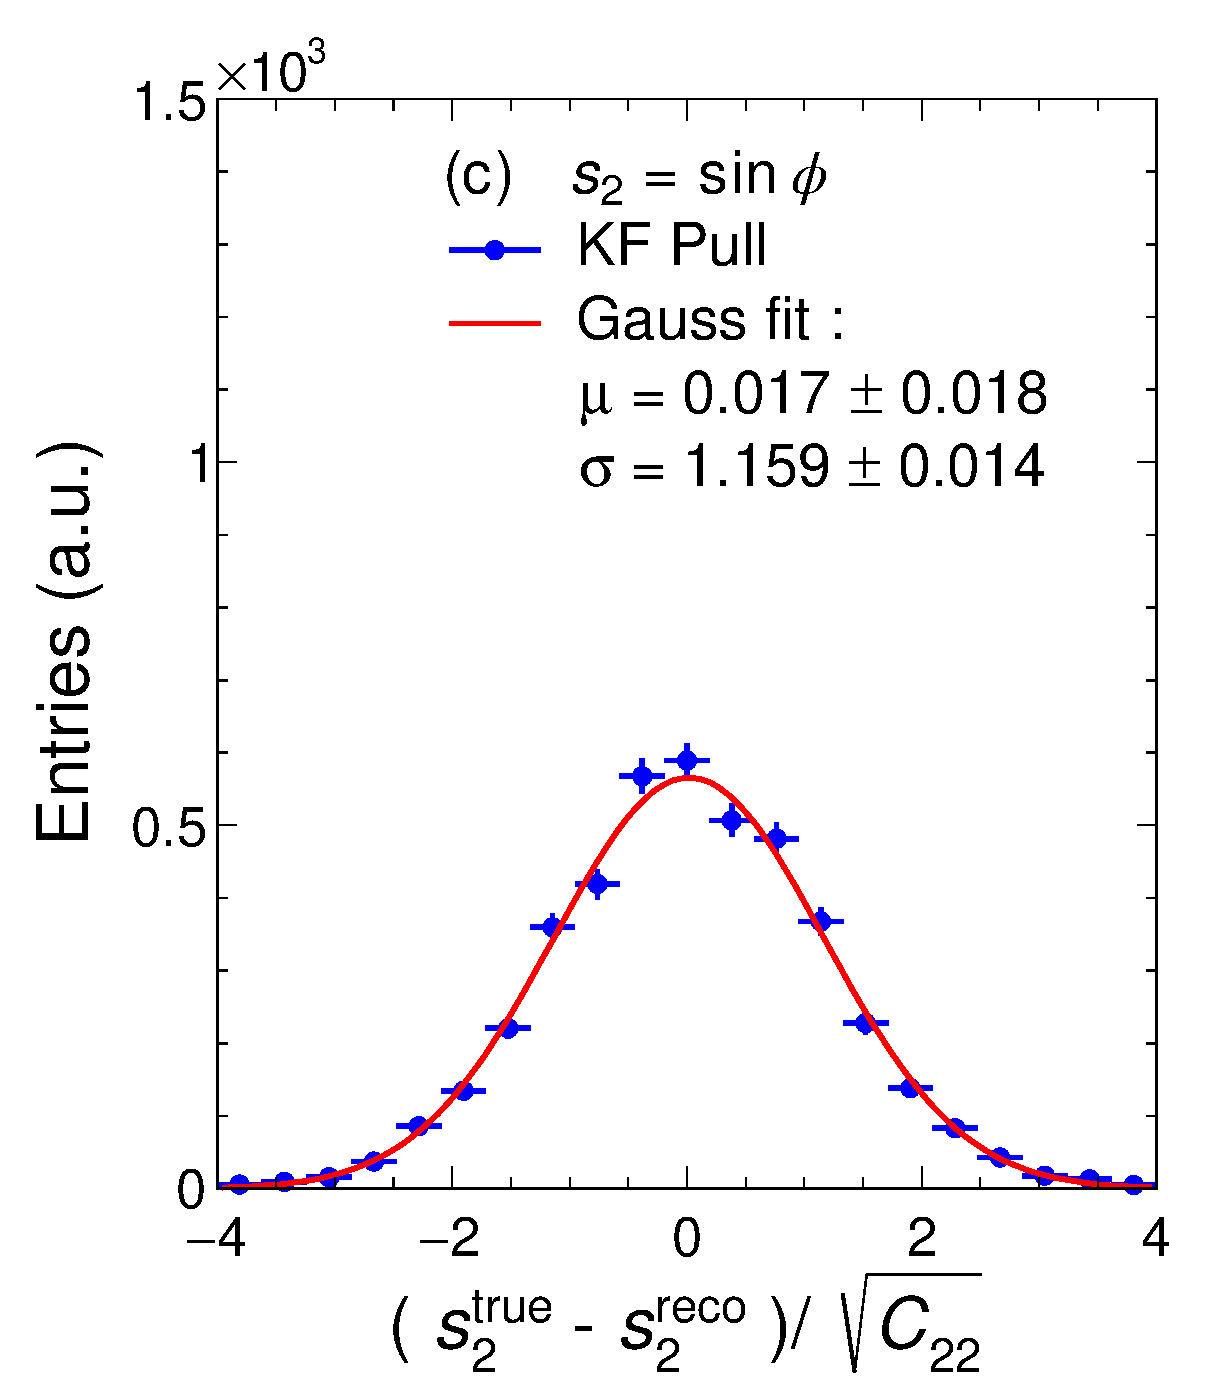
\includegraphics[width=\textwidth]{figures/ch4-KF_NDGArLite/Toy/Corr/UnitKFEnd_p2.eps}
         \caption{}
         \label{fig:resp2KF_GArLite_Corr}
     \end{subfigure}
          \begin{subfigure}{0.32\textwidth}
         \centering
         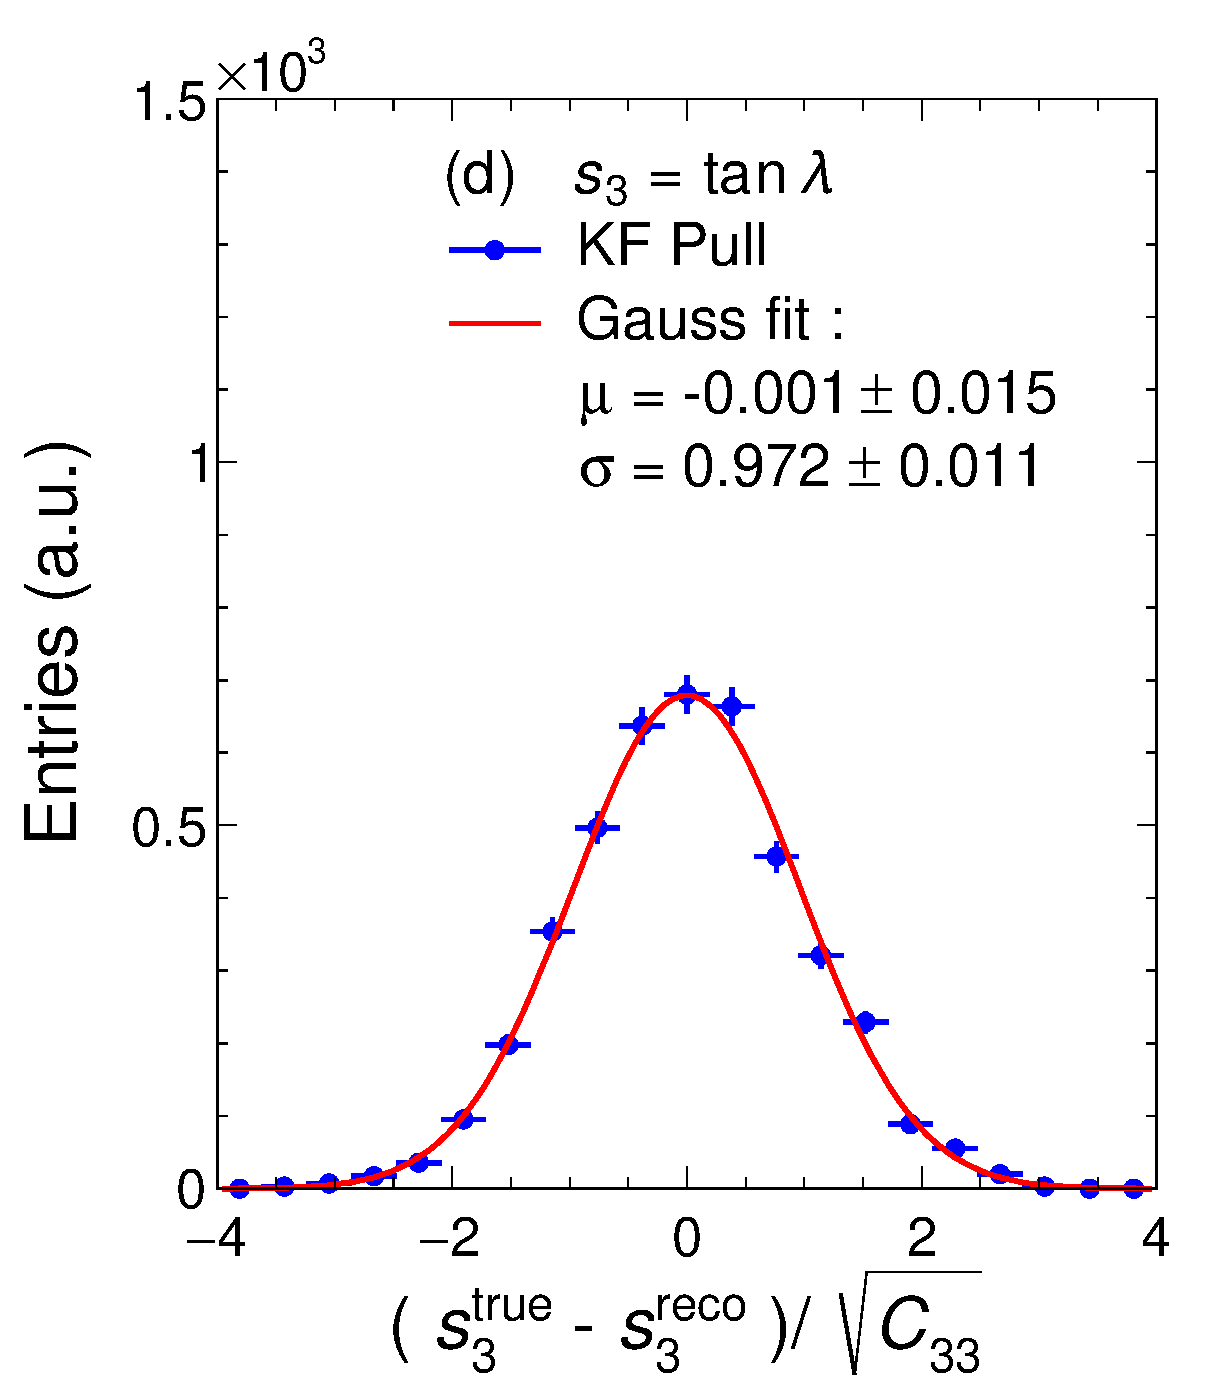
\includegraphics[width=\textwidth]{figures/ch4-KF_NDGArLite/Toy/Corr/UnitKFEnd_p3.eps}
         \caption{}
         \label{fig:resp3KF_GArLite_Corr}
     \end{subfigure}
     \begin{subfigure}{0.32\textwidth}
         \centering
         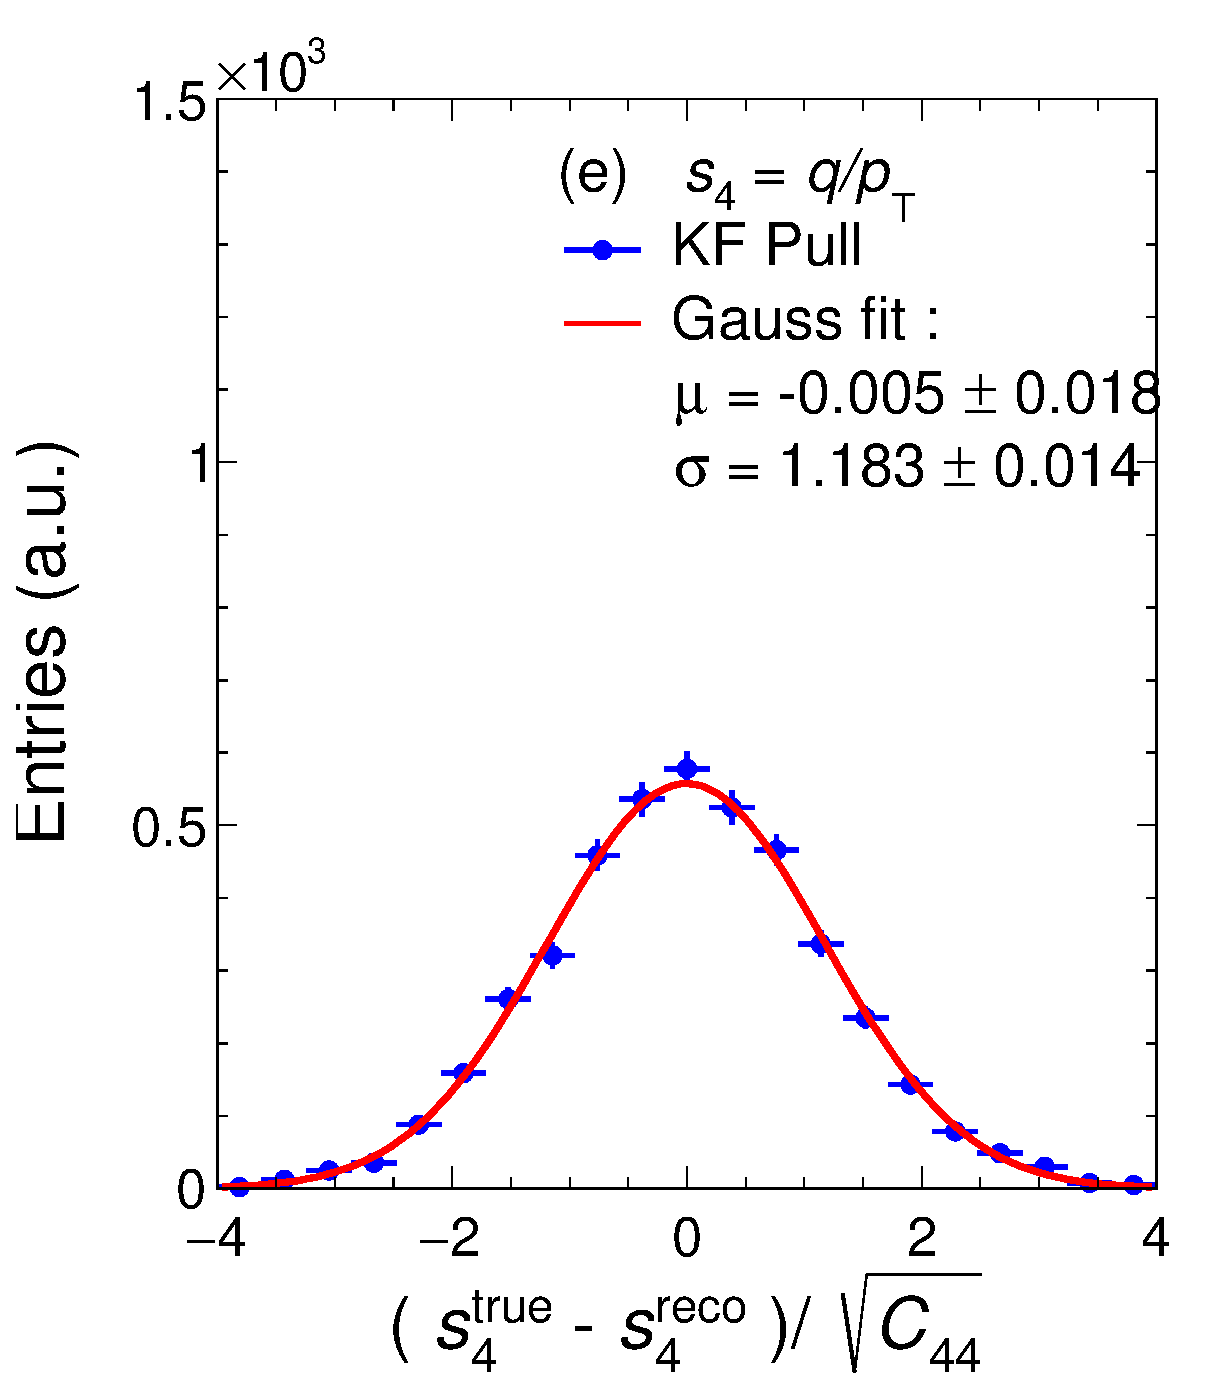
\includegraphics[width=\textwidth]{figures/ch4-KF_NDGArLite/Toy/Corr/UnitKFEnd_p4.eps}
         \caption{}
         \label{fig:resp4KF_GArLite_Corr}
     \end{subfigure}
        \caption[Pull distributions for the \texttt{KF-Lite} algorithm over the Corrected (C) sample.]{Pull distributions for the \texttt{KF-Lite} algorithm over the Corrected (C) sample. All distributions were fitted to a Gaussian function. Results for parameters $s_0$ to $s_4$ (i.e. $y$, $x$, $\sin\phi$, $\tan\lambda$ and $q/p_{\text{T}}$) are shown from left to right and labeled from (a) to (e) accordingly. }
        \label{fig:ToyUnitKF_GArLite_Corr}
\end{figure}

The first test performed on both the NC and C samples was a so-called pull test. A pull, $\Pi$, is defined as the difference between the true value and the reconstructed value of one of the state vector parameters $s=(y,z,\sin{\phi},\tan{\lambda},$ $ q/p_{\text{T}})=(s_0,s_1,s_2,s_3,s_4)$, normalized by the square root of the correspondent diagonal element of the covariance matrix $C_{ii}$:
\begin{equation}
\label{eq:Pull}
    \Pi_i\equiv\frac{s_i-s_i^{\text{true}}}{\sqrt{C_{ii}}}.
\end{equation}
If the covariance matrix is well defined, the distributions of the pulls should be normal, centered in 0  with $\sigma\simeq1$.

The NC sample pulls were tested, both for the \texttt{Seed} and the \texttt{KF-Lite} results were fitted to a standard Gaussian distribution. Note that the pulls for the \texttt{Seed} algorithm were tested at the start of the particle trajectory, while for the \texttt{KF-Lite} they were tested at the end after the full propagation. The resulting NC Sample distributions for all the state vector parameters are shown in Figs.~\ref{fig:ToyUnitSeed_GArLite_NoCorr}  and~\ref{fig:ToyUnitKF_GArLite_NoCorr} for the \texttt{Seed} and the \texttt{KF-Lite} results respectively. A very significant underestimation of the $\tan\lambda$ parameter can be seen in the \texttt{Seed}  results for which we obtain a value of $\sigma$ which is roughly double the expectation. This is not corrected after the \texttt{KF-Lite} propagation, for which significant underestimations can also be seen for $\sin\phi$ and $q/p_T$ parameters. This to be expected, given that the uncertainty contributions that arise from the particles' multiple scattering and energy loss have not been accounted for.

The C sample pulls were tested in an analogous manner and the resulting distributions are shown in in Figs.~\ref{fig:ToyUnitSeed_GArLite_Corr}  and~\ref{fig:ToyUnitKF_GArLite_Corr} for the \texttt{Seed} and the \texttt{KF-Lite} results, respectively. The \texttt{Seed} algorithm produces slight over-estimations on the $\sin\phi$ and $\tan\lambda$ uncertainties. These imperfections however are much less significant that in the case of the NC sample and are almost completely corrected for by the propagation of the \texttt{KF-Lite} for which all Pulls have $\sigma\sim 1$ and $\mu \sim 0$. This means that the energy loss and multiple scattering corrections that we apply to the algorithm are internally consistent with the simulation and allow us to produce correct estimates of the uncertainties of the reconstructed estimates of the state vector parameters.

\begin{figure}[t]
     \centering
     \begin{subfigure}[b]{0.48\textwidth}
         \centering
         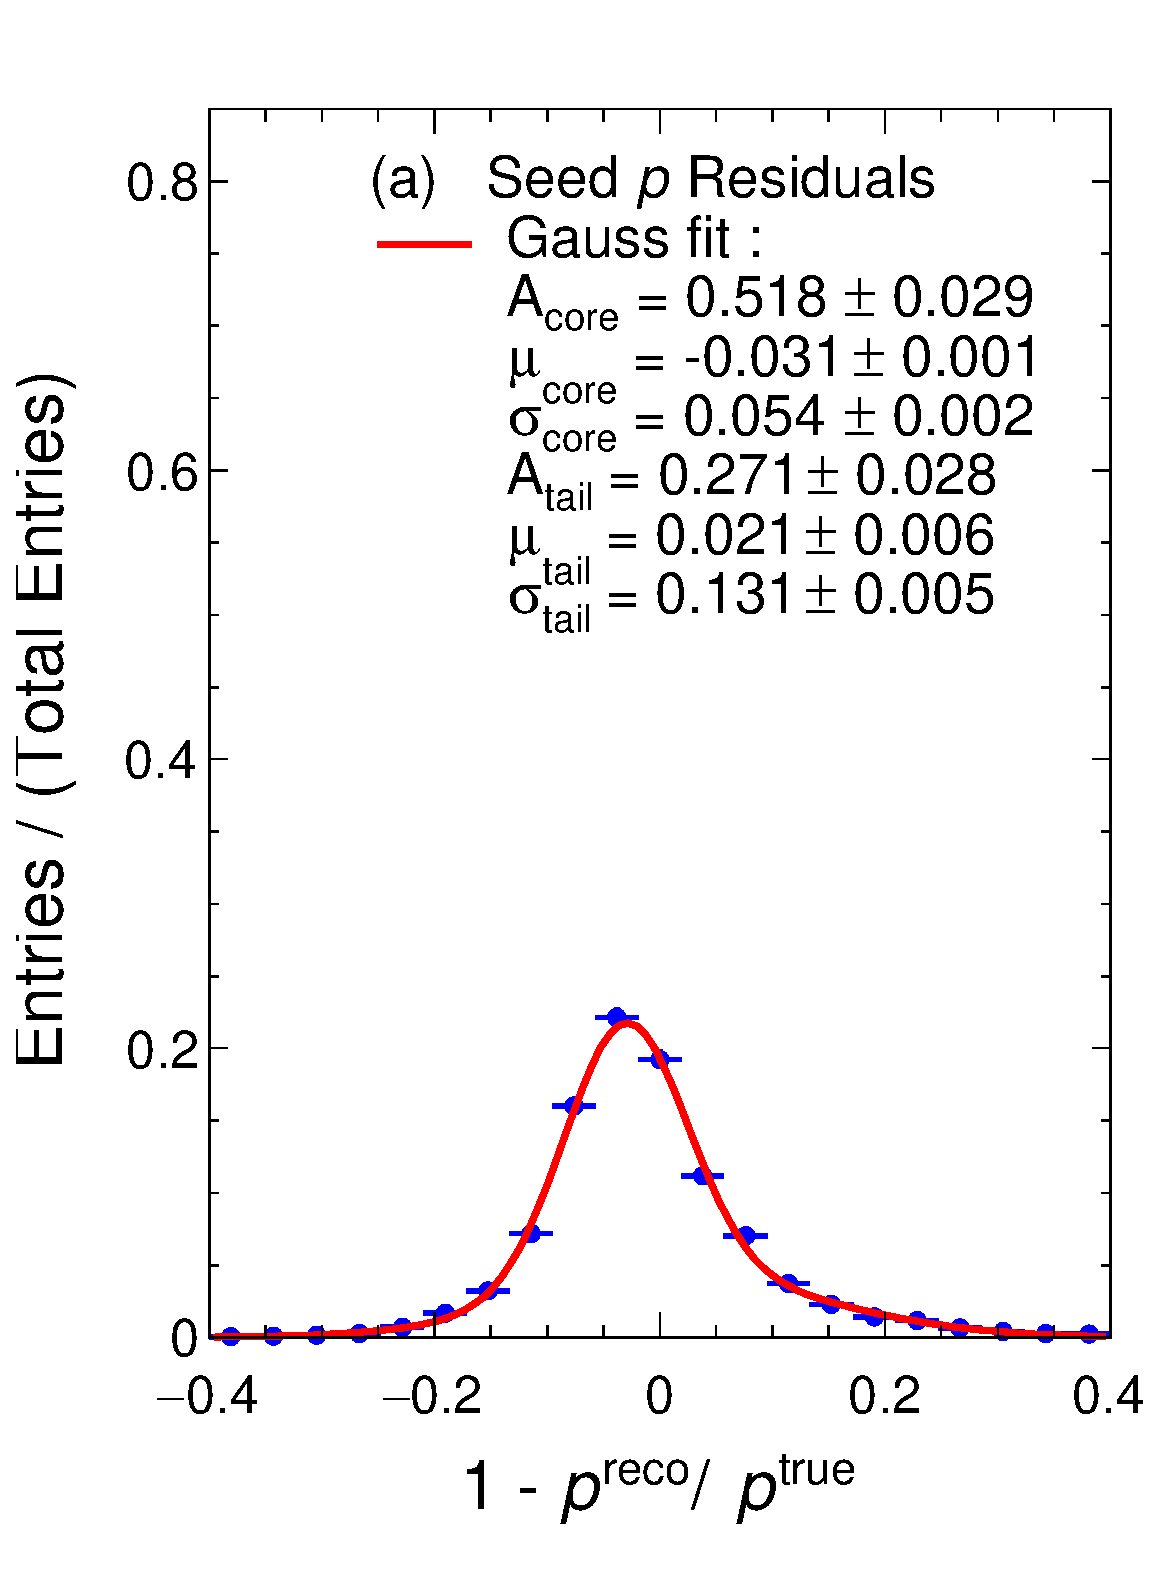
\includegraphics[width=\textwidth]{figures/ch4-KF_NDGArLite/Toy/NoCorr/pRes_doublegauss.eps}
         \caption{}
         \label{fig:ToyResP_GArLite_NoCorr_Seed}
     \end{subfigure}
     \begin{subfigure}[b]{0.48\textwidth}
         \centering
         \includegraphics[width=\textwidth]{figures/ch4-KF_NDGArLite/Toy/NoCorr/pResKF_doublegauss.eps}
         \caption{}
         \label{fig:ToyResP_GArLite_NoCorr_KF}
     \end{subfigure}
        \caption[Momentum fractional residuals for the (a) \texttt{Seed} and (b) \texttt{KF-Lite} algorithms in the NC Toy Monte Carlo sample.]{Momentum fractional residuals $R=p_{\text{reco}}/p_{\text{true}} - 1$ for the (a) \texttt{Seed} and (b) \texttt{KF-Lite} algorithms in the NC Toy Monte Carlo sample. In both cases the distributions were fitted with a double Gaussian function defining a core and a tail distributions.} \label{fig:ToyResP_GArLite_NoCorr}
\end{figure}

For both the NC and C we focused as figures of merit of the total momentum resolution and bias. Both of these quantities can be defined as the $\sigma$ and $\mu$ of a Gaussian fit applied to the momentum fractional residuals:
\begin{equation}
    \label{eq:MomentumRes}
    R = \frac{p_{\text{reco}}}{p_{\text{true}}} - 1.
\end{equation}
In Fig. \ref{fig:ToyResP_GArLite_NoCorr} we show the momentum fractional residual distributions obtained for the \texttt{Seed} and \texttt{KF-Lite} algorithms in the NC sample where the Energy loss and multiple scattering corrections haven't been applied. In both cases the distributions were fitted with a double Gaussian function defining core and tails sub-sets. The \texttt{Seed} algorithm is shown to produce a significant negative bias $\mu_\text{core}=(-3.1\pm0.1)\%$ in the momentum estimation. This is due to an underestimation of the momentum brought by the lack of energy loss correction imparted to the algorithm's estimate. Similarly the \texttt{KF-Lite} residuals shows a positive but much less significant bias $\mu_\text{core}=(0.6\pm0.1)\%$. The opposite direction of the bias is to be expected, since the estimate is produced at the end of the particle trajectory rather than at the start.

\begin{figure}[t]
     \centering
     \begin{subfigure}[b]{0.48\textwidth}
         \centering
         \includegraphics[width=\textwidth]{figures/ch4-KF_NDGArLite/Toy/Corr/pRes_doublegauss.eps}
         \caption{}
         \label{fig:ToyResP_GArLite_Corr_Seed}
     \end{subfigure}
     \begin{subfigure}[b]{0.48\textwidth}
         \centering
         \includegraphics[width=\textwidth]{figures/ch4-KF_NDGArLite/Toy/Corr/pResKF_doublegauss.eps}
         \caption{}
         \label{fig:ToyResP_GArLite_Corr_KF}
     \end{subfigure}
        \caption[Momentum fractional residuals for the (a) \texttt{Seed} and (b) \texttt{KF-Lite} algorithms in the NC Toy Monte Carlo sample.]{Momentum fractional residuals $R=p_{\text{reco}}/p_{\text{true}} - 1$ for the (a) \texttt{Seed} and (b) \texttt{KF-Lite} algorithms in the NC Toy Monte Carlo sample. Similar to Fig. \ref{fig:ToyResP_GArLite_Corr}.} \label{fig:ToyResP_GArLite_Corr}
\end{figure}

In Fig. \ref{fig:ToyResP_GArLite_Corr} we show the momentum fractional residual distributions obtained for the \texttt{Seed} and \texttt{KF-Lite} algorithms in the C sample where the Energy loss and multiple scattering corrections have been applied. In both cases the distributions were fitted with a double Gaussian function analogously to what was done for the NC sample. The bias seen for \texttt{Seed} algorithm in the NC sample is now almost completely corrected having $\mu_\text{core}=(0.3\pm0.1)\%$. Similarly the \texttt{KF-Lite} residuals shows no bias having  $\mu_\text{core}=(0.0\pm 0.1)\%$ . The energy loss correction that we apply to both algorithm is shown to be perfectly consistent with the simulation.

\begin{figure}[t]
     \centering
     \begin{subfigure}[b]{0.42\textwidth}
         \centering
         \includegraphics[width=\textwidth]{figures/ch4-KF_NDGArLite/Toy/RespVSN.eps}
         \caption{}
         \label{fig:ToyResPVSN_GArLite_Res}
     \end{subfigure}
     \begin{subfigure}[b]{0.42\textwidth}
         \centering
         \includegraphics[width=\textwidth]{figures/ch4-KF_NDGArLite/Toy/BiaspVSN.eps}
         \caption{}
         \label{fig:ToyResPVSN_GArLite_Bias}
     \end{subfigure}
     \begin{subfigure}[b]{0.42\textwidth}
         \centering
         \includegraphics[width=\textwidth]{figures/ch4-KF_NDGArLite/Toy/RespVSp.eps}
         \caption{}
         \label{fig:ToyResPVSp_GArLite_Res}
     \end{subfigure}
     \begin{subfigure}[b]{0.42\textwidth}
         \centering
         \includegraphics[width=\textwidth]{figures/ch4-KF_NDGArLite/Toy/BiaspVSp.eps}
         \caption{}
         \label{fig:ToyResPVSp_GArLite_Bias}
     \end{subfigure}
        \caption{Relative momentum resolution $\sigma$ and bias $\mu$ as a function of (a), (b) the number of hit clusters belonging to the track and (c), (d) the initial true momentum of the particle. The results for the NC sample are shown in black while for the C sample are shown in blue } \label{fig:ToyResPVS_GArLite}
\end{figure}



For a more complete view of the results we also show the relative momentum resolution and bias produced by the \texttt{KF-Lite} algorithm as a function of some key track properties. The results for the NC and C sample are shown in black and blue respectively.  In Fig. \ref{fig:ToyResPVS_GArLite} we show the two quantities as a function of the number of hit clusters belonging to the track $N$ (Figs. \ref{fig:ToyResPVSN_GArLite_Bias} and \ref{fig:ToyResPVSN_GArLite_Res})the particle's initial true momentum $p^\texttt{true}$ (Figs. \ref{fig:ToyResPVSp_GArLite_Bias} and \ref{fig:ToyResPVSp_GArLite_Res}). Note that in both of these cases the $\mu$ and $\sigma$ values are taken from a simple Gaussian fit, rather that a double Gaussian fit as was done for Figs. \ref{fig:ToyResP_GArLite_NoCorr} and \ref{fig:ToyResP_GArLite_Corr}. It is clear from a direct comparison of the two samples that while the results are comparable in terms of resolution, a significant bias correction in the momentum reconstruction is achieved by the application of the energy loss correction step to the \texttt{KF-Lite}. 

The dependency of the momentum resolution on $p$ and $N$ can be predicted by using the Gluckstern formulas, which describe the dependency of a curvature measurement resolution on several track parameters \cite{PDG:34}. Adapting the formulas to get the total momentum dependency we get:
\begin{equation}\label{eq:sigmaNptot}
\frac{\sigma_{\text{H}}(p)}{p}=\frac{\cos\lambda \ p  \ \sigma_{r\phi}}{0.3 BL_\textrm{Arm}^2}\sqrt{\frac{720}{N+4}}.
\end{equation}
\begin{equation}\label{eq:sigmaMSptot}
\frac{\sigma_{\text{MS}}(p)}{p}=\frac{0.016 \ (\textrm{GeV}/c)}{0.3 B l\beta \cos \lambda}\sqrt{\frac{l}{X_0}},
\end{equation}
where $\sigma_{\text{H}}(p)$ is the point resolution component of the total momentum resolution and $\sigma_{\text{MS}}(p)$ is the multiple scattering component. The total resolution is expected to be:
\begin{equation}
    \sigma_\text{tot}(p)=\sqrt{\sigma_\text{H}^2+\sigma_\text{MS}^2}
\end{equation}
The multiple scattering component $\sigma_\text{MS}$ is dominant at lower momenta, while the hit component $\sigma_\text{H}$ is dominant at higher momenta. This dependency can be clearly seen in Fig. \ref{fig:ToyResPVSp_GArLite_Res} where at lower momenta the resolution has an inverse proportionality on the momentum, which directly derives from the $\beta$ at the denominator present in Eq. \ref{eq:sigmaMSptot}, while at higher momenta the direct proportionality seen in Eq. \ref{eq:sigmaNptot} dominates. In Fig. \ref{fig:ToyResPVSN_GArLite_Res} on the other hand we clearly see the $\propto 1/\sqrt{N}$ dependency that we expect from Eq. \ref{eq:sigmaNptot}

\section{The \texttt{GArSoft} simulation studies}
\label{Sec:MC-Studies-Lite}

\begin{figure}[t]
     \centering
     \includegraphics[width=0.6\textwidth]{figures/ch4-KF_NDGArLite/MC/EvtDisplay.png}
     \caption[\texttt{GArsoft} event display showing a muon produced with the particle gun feature.]{\texttt{GArsoft} event display showing a muon produced with the particle gun feature and used for the Lite-1 and Lite-2 studies. The layout of the tracker area is outlined in white and the trajectory of the muon is shown in blue. }
        \label{fig:GArLiteMuonEvent}
\end{figure} 

The \texttt{GArSoft} software suite described in Sec. \ref{Sec:GArSoft_Lite} was used to construct a particle sample to test the performance of the new Kalman Filter algorithm and compare it to the \texttt{ILRM} algorithm which represented the standard reconstruction fit at the time. The simulation was conducted using the Geant4 particle gun tool and using the 6-plane ND-GAr-Lite geometry. The sample was mono-energetic, containing muons having the same initial momenta $p=1\ \text{GeV}/c$ and starting position in the front and center of the first scintillator tracking planes.  All particles were simulated to have a forward going momentum, with randomized small $y$ and $z$ components. These limited initial conditions were chosen for the simplicity of production and implementation with the \texttt{KF-Lite} algorithm. They were also chosen to be a relatively close match with the conditions of muons coming from ND-LAr which are the main sample of interest for ND-GAr-Lite. An example \texttt{GArSoft} event display for one of these simulated events is shown in Fig. \ref{fig:GArLiteMuonEvent} .  

Similarly to the toy MC studies described in the previous section many aspects of the reconstruction algorithm could be switched on and off modularly, in order to be tested individually. These feature include the energy loss and multiple scattering corrections which can be applied to both the seeding algorithm and the \texttt{KF-Lite}. Additionally two separate types of seeding algorithm were implemented: the \texttt{Seed} algorithm as well as the \texttt{ILRM} algorithm. 

\begin{figure}[t]
     \centering
     \begin{subfigure}[b]{0.48\textwidth}
         \centering
         \includegraphics[width=\textwidth]{figures/ch4-KF_NDGArLite/MC/LengthAllTall.eps}
         \caption{}
         \label{fig:MCGArLite_L}
     \end{subfigure}
     \begin{subfigure}[b]{0.48\textwidth}
         \centering
         \includegraphics[width=\textwidth]{figures/ch4-KF_NDGArLite/MC/NPointsAllTall.eps}
         \caption{}
         \label{fig:MCGArLite_N}
     \end{subfigure}
        \caption[Properties of the particles simulated for the \texttt{GArSoft} Lite-1 and Lite-2 samples.]{Properties of the particles simulated for the \texttt{GArSoft} Lite-1 and Lite-2 samples: (a) length of the particle tracks $L$ (cm) measured as the summed distances between the hit clusters; (b) number of hit clusters belonging to the tracks $N$.} \label{fig:MCGArLite_prop}
\end{figure}

\begin{figure}[t]
     \centering
     \begin{subfigure}{0.32\textwidth}
         \centering
         \includegraphics[width=\textwidth]{figures/ch4-KF_NDGArLite/MC/ALICE+KF/UnitSeed_p0.eps}
         \caption{}
         \label{fig:resp0Seed_GArLite_ALICE+KF}
     \end{subfigure}
     \begin{subfigure}{0.32\textwidth}
         \centering
         \includegraphics[width=\textwidth]{figures/ch4-KF_NDGArLite/MC/ALICE+KF/UnitSeed_p1.eps}
         \caption{}
         \label{fig:resp1Seed_GArLite_ALICE+KF}
     \end{subfigure}
    \begin{subfigure}{0.32\textwidth}
         \centering
         \includegraphics[width=\textwidth]{figures/ch4-KF_NDGArLite/MC/ALICE+KF/UnitSeed_p2.eps}
         \caption{}
         \label{fig:resp2Seed_GArLite_ALICE+KF}
     \end{subfigure}
          \begin{subfigure}{0.32\textwidth}
         \centering
         \includegraphics[width=\textwidth]{figures/ch4-KF_NDGArLite/MC/ALICE+KF/UnitSeed_p3.eps}
         \caption{}
         \label{fig:resp3Seed_GArLite_ALICE+KF}
     \end{subfigure}
     \begin{subfigure}{0.32\textwidth}
         \centering
         \includegraphics[width=\textwidth]{figures/ch4-KF_NDGArLite/MC/ALICE+KF/UnitSeed_p4.eps}
         \caption{}
         \label{fig:resp4Seed_GArLite_ALICE+KF}
     \end{subfigure}
        \caption[Pull distributions for the \texttt{Seed} algorithm over the Lite-1 sample.]{Pull distributions for the \texttt{Seed} algorithm over the Lite-1 sample. All distributions were fitted to a Gaussian function. Results for parameters $s_0$ to $s_4$ (i.e. $y$, $x$, $\sin\phi$, $\tan\lambda$ and $q/p_{\text{T}}$) are shown from left to right and labeled from (a) to (e) accordingly. }
        \label{fig:MCUnitSeed_GArLite_ALICE+KF}
\end{figure}

In this section we focus on the results obtained for the two most complete and best performing combinations of the algorithm correspond to samples 15.5.2c and 15.5.6c in Tab. \ref{Tab:Lite} in App. \ref{App:Summary_Tables}. In both cases we use the same \texttt{KF-Lite} algorithm and the full set of material budget corrections are applied, but the two samples are differentiated by the seeding strategy: the \texttt{Seed} method in the first case, the \texttt{ILRM} in the second. These two test sample conditions will be referred to as sample Lite-1 and sample Lite-2 respectively. Some key properties of the particle tracks which are common to both samples are shown in Fig. \ref{fig:MCGArLite_prop}, specifically the length of the tracks $L$ as defined in Sec. \ref{Sec:ToyMCTests-Lite} and the number of hit clusters belonging to the particle track $N$. Comparing the properties with those shown in Fig. \ref{fig:ToyGArLite_prop} it's clear that the Toy Monte Carlo simulation produced results that are very close to the more complete simulation available in \texttt{GArSoft}.

Similarly to what was done within the toy Monte Carlo study, pull-tests were performed for both the seeding algorithm (which include both the \texttt{Seed} and the \texttt{ILRM}) and the \texttt{KF-Lite} algorithm after the full propagation. Note that in this case both results are taken at the start of the muon track, for ease of comparison with the \texttt{GArSoft} reconstruction results. This is because, while the Kalman Filter was always applied twice, producing estimates at both end of the track, the original \texttt{ILRM} reconstruction was only applied once, producing a single estimation at the start of the track. 


\begin{figure}[t]
     \centering
     \begin{subfigure}{0.32\textwidth}
         \centering
         \includegraphics[width=\textwidth]{figures/ch4-KF_NDGArLite/MC/ALICE+KF/UnitKFEnd_p0.eps}
         \caption{}
         \label{fig:resp0KF_GArLite_ALICE+KF}
     \end{subfigure}
     \begin{subfigure}{0.32\textwidth}
         \centering
         \includegraphics[width=\textwidth]{figures/ch4-KF_NDGArLite/MC/ALICE+KF/UnitKFEnd_p1.eps}
         \caption{}
         \label{fig:resp1KF_GArLite_ALICE+KF}
     \end{subfigure}
    \begin{subfigure}{0.32\textwidth}
         \centering
         \includegraphics[width=\textwidth]{figures/ch4-KF_NDGArLite/MC/ALICE+KF/UnitKFEnd_p2.eps}
         \caption{}
         \label{fig:resp2KF_GArLite_ALICE+KF}
     \end{subfigure}
          \begin{subfigure}{0.32\textwidth}
         \centering
         \includegraphics[width=\textwidth]{figures/ch4-KF_NDGArLite/MC/ALICE+KF/UnitKFEnd_p3.eps}
         \caption{}
         \label{fig:resp3KF_GArLite_ALICE+KF}
     \end{subfigure}
     \begin{subfigure}{0.32\textwidth}
         \centering
         \includegraphics[width=\textwidth]{figures/ch4-KF_NDGArLite/MC/ALICE+KF/UnitKFEnd_p4.eps}
         \caption{}
         \label{fig:resp4KF_GArLite_ALICE+KF}
     \end{subfigure}
        \caption[Pull distributions for the \texttt{KF-Lite} algorithm over the Lite-1 sample where the \texttt{Seed} algorithm was used.]{Pull distributions for the \texttt{KF-Lite} algorithm over the Lite-1 sample where the \texttt{Seed} algorithm was used. All distributions were fitted to a Gaussian function. Results for parameters $s_0$ to $s_4$ (i.e. $y$, $x$, $\sin\phi$, $\tan\lambda$ and $q/p_{\text{T}}$) are shown from left to right and labeled from (a) to (e) accordingly. }
        \label{fig:MCUnitKFEnd_GArLite_ALICE+KF}
\end{figure}

\begin{figure}[t]
     \centering
     \begin{subfigure}{0.32\textwidth}
         \centering
         \includegraphics[width=\textwidth]{figures/ch4-KF_NDGArLite/MC/ILRM+KF/UnitSeed_p0.eps}
         \caption{}
         \label{fig:resp0Seed_GArLite_ILRM+KF}
     \end{subfigure}
     \begin{subfigure}{0.32\textwidth}
         \centering
         \includegraphics[width=\textwidth]{figures/ch4-KF_NDGArLite/MC/ILRM+KF/UnitSeed_p1.eps}
         \caption{}
         \label{fig:resp1Seed_GArLite_ILRM+KF}
     \end{subfigure}
    \begin{subfigure}{0.32\textwidth}
         \centering
         \includegraphics[width=\textwidth]{figures/ch4-KF_NDGArLite/MC/ILRM+KF/UnitSeed_p2.eps}
         \caption{}
         \label{fig:resp2Seed_GArLite_ILRM+KF}
     \end{subfigure}
          \begin{subfigure}{0.32\textwidth}
         \centering
         \includegraphics[width=\textwidth]{figures/ch4-KF_NDGArLite/MC/ILRM+KF/UnitSeed_p3.eps}
         \caption{}
         \label{fig:resp3Seed_GArLite_ILRM+KF}
     \end{subfigure}
     \begin{subfigure}{0.32\textwidth}
         \centering
         \includegraphics[width=\textwidth]{figures/ch4-KF_NDGArLite/MC/ILRM+KF/UnitSeed_p4.eps}
         \caption{}
         \label{fig:resp4Seed_GArLite_ILRM+KF}
     \end{subfigure}
        \caption[Pull distributions for the \texttt{ILRM} algorithm over the Lite-2 sample]{Pull distributions for the \texttt{ILRM} algorithm over the Lite-2 sample. All distributions were fitted to a Gaussian function. Results for parameters $s_0$ to $s_4$ (i.e. $y$, $x$, $\sin\phi$, $\tan\lambda$ and $q/p_{\text{T}}$) are shown from left to right and labeled from (a) to (e) accordingly. }
        \label{fig:MCUnitSeed_GArLite_ILRM+KF}
\end{figure}

\begin{figure}[t]
     \centering
     \begin{subfigure}{0.32\textwidth}
         \centering
         \includegraphics[width=\textwidth]{figures/ch4-KF_NDGArLite/MC/ILRM+KF/UnitKFEnd_p0.eps}
         \caption{}
         \label{fig:resp0KF_GArLite_ILRM+KF}
     \end{subfigure}
     \begin{subfigure}{0.32\textwidth}
         \centering
         \includegraphics[width=\textwidth]{figures/ch4-KF_NDGArLite/MC/ILRM+KF/UnitKFEnd_p1.eps}
         \caption{}
         \label{fig:resp1KF_GArLite_ILRM+KF}
     \end{subfigure}
    \begin{subfigure}{0.32\textwidth}
         \centering
         \includegraphics[width=\textwidth]{figures/ch4-KF_NDGArLite/MC/ILRM+KF/UnitKFEnd_p2.eps}
         \caption{}
         \label{fig:resp2KF_GArLite_ILRM+KF}
     \end{subfigure}
          \begin{subfigure}{0.32\textwidth}
         \centering
         \includegraphics[width=\textwidth]{figures/ch4-KF_NDGArLite/MC/ILRM+KF/UnitKFEnd_p3.eps}
         \caption{}
         \label{fig:resp3KF_GArLite_ILRM+KF}
     \end{subfigure}
     \begin{subfigure}{0.32\textwidth}
         \centering
         \includegraphics[width=\textwidth]{figures/ch4-KF_NDGArLite/MC/ILRM+KF/UnitKFEnd_p4.eps}
         \caption{}
         \label{fig:resp4KF_GArLite_ILRM+KF}
     \end{subfigure}
        \caption[Pull distributions for the \texttt{KF-Lite} algorithm over the Lite-2 sample where the \texttt{ILRM} algorithm was used.]{Pull distributions for the \texttt{KF-Lite} algorithm over the Lite-2 sample where the \texttt{ILRM} algorithm was used. All distributions were fitted to a Gaussian function. Results for parameters $s_0$ to $s_4$ (i.e. $y$, $x$, $\sin\phi$, $\tan\lambda$ and $q/p_{\text{T}}$) are shown from left to right and labeled from (a) to (e) accordingly. }
        \label{fig:MCUnitKFEnd_GArLite_ILRM+KF}
\end{figure}

The pull distributions for all the state vector parameters obtained using the \texttt{Seed} algorithm are shown in Fig. \ref{fig:MCUnitSeed_GArLite_ALICE+KF}. All pulls are fitted with simple Gaussian distribution showing no biases and $\sigma\sim1$. A somewhat significant over-estimation of the uncertainties can be seen for parameters $s_2=\sin\phi$ and $s_3=\tan\lambda$. This was also seen in Fig. \ref{fig:ToyUnitSeed_GArLite_Corr} and is consistent with previous test results. 

In Fig. \ref{fig:MCUnitKFEnd_GArLite_ALICE+KF} we show the pulls obtained after the full propagation of the \texttt{KF-Lite} algorithm. In this case the over-estimation seen for $s_2=\sin\phi$ and $s_3=\tan\lambda$ is fully corrected for, but a slight over-estimation on parameter $s_4=q/p_\texttt{T}$ which was not seen in the equivalent toy Monte Carlo test (see Fig. \ref{fig:ToyUnitKF_GArLite_Corr}) is introduced. 

To produce these results an ad-hoc correction to the multiple scattering calculation step of the \texttt{KF-Lite} reconstruction was introduced. This correction is applied in those propagation steps where the two consecutive hit clusters belong to different tracking planes and the particle is moving between them. In the toy Monte Carlo the space between the tracking planes was simulated to be completely empty, while in the more realistic geometry used by \texttt{GArSoft}, they are filled with air at atmospheric pressure. The propagation of the particles in these passive portions of the detector produces additional multiple scattering uncertainties that, while small compared to the impact of the scintillator planes, are not completely negligible. In order to compensate for this underestimation a multiplicative factor of 4 is applied to the $Q$ matrix described in Eq. \ref{eq:Q}. This factor was found by trial and error and was shown to produce the best pulls overall. A more proper treatment would have required to apply an additional correction step calculating the length of the trajectory between the planes and using the material properties of air. However this was not attempted as the ad hoc correction already showed satisfactory results. 

The pull distributions obtained using the \texttt{ILRM} algorithm as the seeding algorithm  are shown in Fig. \ref{fig:MCUnitSeed_GArLite_ILRM+KF}. While the results don't show any bias the $\sigma$ values for parameters $s_2=\sin\phi$, $s_3=\tan\lambda$ and $s_4=q/p_\text{T}$ are largely over-estimated by a factor of $\sim2$. This is in line with the expectations for the reasons outlined in Section \ref{Sec:SeedingLite}. Specifically the fact that the method used for the calculation of the $C_0$ matrix is only valid if just three points are used for the estimate, as it was intended for the \texttt{Seed} method. 

After the full propagation of the \texttt{KF-Lite} algorithm the over-estimation in the pulls are largely corrected for. This can be seen in Fig. \ref{fig:MCUnitKFEnd_GArLite_ILRM+KF} were the pulls are shown for the \texttt{KF-Lite} algorithm in the Lite-2 sample. All the $\sigma$ are very close to 1 with the exception of $s_4=q/p_\text{T}$ for which a somewhat significant under-estimation is seen. Note that the ad-hoc treatment needed for the propagation in air described for the Lite-1 sample was also used in this case. 

\begin{figure}[t]
     \centering
     \begin{subfigure}{0.32\textwidth}
         \centering
         \includegraphics[width=\textwidth]{figures/ch4-KF_NDGArLite/MC/ALICE+KF/pResKF_doublegauss.eps}
         \caption{}
         \label{fig:respKF_GArLite_ALICE+KF}
     \end{subfigure}
     \begin{subfigure}{0.32\textwidth}
         \centering
         \includegraphics[width=\textwidth]{figures/ch4-KF_NDGArLite/MC/ILRM+KF/pResKF_doublegauss.eps}
         \caption{}
         \label{fig:respKF_GArLite_ILRM+KF}
     \end{subfigure}
    \begin{subfigure}{0.32\textwidth}
         \centering
         \includegraphics[width=\textwidth]{figures/ch4-KF_NDGArLite/MC/ILRM+KF/pResILRM_doublegauss.eps}
         \caption{}
         \label{fig:respKF_GArLite_ILRM}
     \end{subfigure}
        \caption[Momentum fractional residuals for the \texttt{KF-Lite} in the Lite-1 and Lite-2 sample compared with the old reconstruction.]{Momentum fractional residuals $R=p_{\text{reco}}/p_{\text{true}} - 1$ for the (a) \texttt{KF-Lite} paired with the 3-points \texttt{Seed} method in the Lite-1 sample (b) \texttt{KF-Lite} paired with the \texttt{ILRM} algorithm in the Lite-2 sample (c) the original \texttt{GArSoft} reconstruction which consists of the \texttt{ILRM} algorithm without any material budget corrections. In all cases the distributions were fitted with a double Gaussian function defining a core and a tail distributions.} 
        \label{fig:MCpResComparison}
\end{figure}

\begin{figure}[t]
     \centering
     \begin{subfigure}[b]{0.48\textwidth}
         \centering
         \includegraphics[width=\textwidth]{figures/ch4-KF_NDGArLite/MC/RespVSN.eps}
         \caption{}
         \label{fig:MCResPVSN_GArLite_Res}
     \end{subfigure}
     \begin{subfigure}[b]{0.48\textwidth}
         \centering
         \includegraphics[width=\textwidth]{figures/ch4-KF_NDGArLite/MC/BiaspVSN.eps}
         \caption{}
         \label{fig:MCResPVSN_GArLite_Bias}
     \end{subfigure}
        \caption[Relative momentum resolution $\sigma$ (a) and bias $\mu$ (b) as a function of the number of hit clusters belonging to the track $N$.]{Relative momentum resolution $\sigma$ (a) and bias $\mu$ (b) as a function of the number of hit clusters belonging to the track $N$. The results are shown in black for the Lite-1 sample, in blue for the Lite-2 sample and in red for the original reconstruction produced with GArSoft.} \label{fig:MCResPVSN_GArLite}
\end{figure}

For both the Lite-1 and Lite-2 we studied the total momentum resolution and bias. Both of these quantities can be defined as the $\sigma$ and $\mu$ of a Gaussian fit applied to the momentum fractional residuals $R$ as defined in Eq. \ref{eq:MomentumRes}. 
We also compared the results with the original fit results available from \texttt{GArSoft}, which were produced with the \texttt{ILRM} algorithm without any material budget correction. In Fig. \ref{fig:MCpResComparison} we show the residuals distributions for the Lite-1, Lite-2 and \texttt{ILRM} standalone algorithms. In all cases the distributions are fitted with a double Gaussian defining a core and tail distribution as it was done for the toy Monte Carlo results. The residuals produced with the original reconstruction method are presented in Fig. \ref{fig:respKF_GArLite_ILRM} and show a very clear bias, that for the core distribution amounts to $\mu_\text{core}= -4\%$. This bias is introduced by the lack of corrections for the energy loss of the particle and it's comparable to what was seen for the NC sample \texttt{Seed} results in the Toy MC study. The residual distributions produced both with the Lite-1 and Lite-2 versions of the algorithm, which are shown in Fig. \ref{fig:respKF_GArLite_ALICE+KF} and \ref{fig:respKF_GArLite_ILRM+KF} show no significant bias, while maintaining essentially identical resolutions to the original \texttt{GArSoft} method.

The relative momentum resolution and bias are also shown as a function of the number of points in the particle tracks $N$ in Fig. \ref{fig:MCResPVSN_GArLite_Res} and \ref{fig:MCResPVSN_GArLite_Bias} respectively. The two quantities are taken as the $\mu$ and $\sigma$ of a simple Gaussian fit of the fractional momentum residual distributions. In black we show the results for the Lite-1 algorithm, in blue for the Lite-2 and in red for the original method. It is clear that no difference is present in terms of resolution, while for the bias the new algorithms largely outperform the old one. Additionally a somewhat significant preference is shown in terms of bias reduction with the Lite-1 algorithm compared to Lite-2. This is likely due to the better pulls produced by the \texttt{Seed} algorithm, which make the \texttt{KF-Lite} more stable.




% \begin{figure}[!ht]
%      \centering
%      \begin{subfigure}{0.32\textwidth}
%          \centering
%          \includegraphics[width=\textwidth]{figures/ch4-KF_NDGArLite/MC/ALICE+KF/sinPhiResKF_doublegauss.eps}
%          \caption{}
%          \label{fig:sinPhiResKF_GArLite_ALICE+KF}
%      \end{subfigure}
%      \begin{subfigure}{0.32\textwidth}
%          \centering
%          \includegraphics[width=\textwidth]{figures/ch4-KF_NDGArLite/MC/ILRM+KF/sinPhiResKF_doublegauss.eps}
%          \caption{}
%          \label{fig:sinPhiResKF_GArLite_ILRM+KF}
%      \end{subfigure}
%     \begin{subfigure}{0.32\textwidth}
%          \centering
%          \includegraphics[width=\textwidth]{figures/ch4-KF_NDGArLite/MC/ILRM+KF/sinPhiResILRM_doublegauss.eps}
%          \caption{}
%          \label{fig:sinPhiResKF_GArLite_ILRM}
%      \end{subfigure}
%         \caption{p Residuals comparisons}
%         \label{fig:MCsinPhiResComparison}
% \end{figure}

% \begin{figure}[!ht]
%      \centering
%      \begin{subfigure}{0.32\textwidth}
%          \centering
%          \includegraphics[width=\textwidth]{figures/ch4-KF_NDGArLite/MC/ALICE+KF/tanlambdaResKF_doublegauss.eps}
%          \caption{}
%          \label{fig:tanlambdaResKF_GArLite_ALICE+KF}
%      \end{subfigure}
%      \begin{subfigure}{0.32\textwidth}
%          \centering
%          \includegraphics[width=\textwidth]{figures/ch4-KF_NDGArLite/MC/ILRM+KF/tanlambdaResKF_doublegauss.eps}
%          \caption{}
%          \label{fig:tanlambdaResKF_GArLite_ILRM+KF}
%      \end{subfigure}
%     \begin{subfigure}{0.32\textwidth}
%          \centering
%          \includegraphics[width=\textwidth]{figures/ch4-KF_NDGArLite/MC/ILRM+KF/tanlambdaResILRM_doublegauss.eps}
%          \caption{}
%          \label{fig:tanlambdaResKF_GArLite_ILRM}
%      \end{subfigure}
%         \caption{p Residuals comparisons}
%         \label{fig:MCtanlambdaResComparison}
% \end{figure}






\begin{savequote}[8cm]
\end{savequote}

\chapter{\label{ch:5-KF-NDGArToy}Kalman Filter Reconstruction for ND-GAr}

\minitoc

\section{The Toy Monte Carlo simulation: fastMCKalman}
\section{The full simulation}
\subsection{The TPC signal formation and digitization}
\subsection{The previously available reconstruction}
\section{The Kalman Filter Applied to ND-GAr}
\section{The toy Monte Carlo study}
\subsection{Validation and methodology}
\subsection{The on and off method}
\subsection{The parameter scan Study}
\subsection{The high pressure study}
\section{Implementation in garsoft}
\subsection{Validation and methodology}
\subsection{Comparison and results}
\begin{savequote}[8cm]
\end{savequote}

\chapter{\label{ch:6-TKI}Transverse Kinematic Imbalance}


\minitoc
\section{Definition of the TKI variables}
\section{Nuclear effects and dependency on the TKI Variables}
\subsection{An hydrogen sample from a high pressure gas TPC}
\section{Hydrogen sample in ND-GAr}
\subsection{Selections and cuts}
\subsection{$\delta p_\textrm{CC}$ resolution}
\subsection{Efficiency and purity}
% \section{Alternative gas mixtures}
% \subsection{Key properties}
% \subsection{Custom simulation in garsoft}
% \subsection{$\delta p_\textrm{CC}$ resolution for different gasses}
% \subsection{Efficiency and Purity for different gasses}
\begin{savequote}[8cm]
\end{savequote}

\chapter*{\label{ch:10-End}Conclusions}

The main goal of this thesis was to describe the development of a novel Kalman Filter algorithm for the ND-GAr detector and show its impact in achieving the detector's physics goals, specifically in the study of neutrino interactions and nuclear effects. 

In Ch. \ref{ch:4-KF-NDGArLite} we introduced the Kalman Filter technique and its application to particle tracking and we described the development and testing of a KF for the ND-GAr-Lite detector named \texttt{KF-Lite}. The ND-GAr-Lite detector was a proposed temporary muon spectrometer designed to substitute ND-GAr in the early days of DUNE experiment's data tacking. The testing of \texttt{KF-Lite} started with the production of a toy Monte Carlo Tool, which allowed to validate each component of the algorithm individually. Once the algorithm was demonstrated to be mature and internally consistent, it was applied to data simulated with \texttt{GArSoft}, the software tool developed by the ND-GAr collaboration. The performance of \texttt{KF-Lite} was tested on a sample of mono-energetic forward-going muons and was compared with the previously available reconstruction algorithm which consisted of an interative linear regression method \texttt{ILRM}. \texttt{KF-Lite} was shown to significantly outperform the \texttt{ILRM}, fully removing a $\sim4\%$ momentum bias present in the original reconstruction.

In Ch. \ref{ch:5-KF-NDGArToy} we described a novel Kalman Filter constructed for the ND-GAr detector and based on the parametrization and the infrastructure originally developed by the ALICE experiment. The new algorithm, which we named the Complete Kalman Filter or \texttt{CKF}, includes a novel feature which allows for the reconstruction of very long \enquote{looping} tracks produced by low energy light particles. The impact of this technique and the internal consistency of the algorithm was demonstrated in a toy Monte Carlo study using a wide range of detector and particle characteristics. In particular it was shown that the novel \enquote{loop-following} method has the potential of improving both the detection efficiency and the resolution significantly for light particles such as electrons, muons and pions. Once the algorithm was demonstrated to be fully mature, it was integrated in \texttt{GArSoft}. Two studies were produced which employed a sample of primary particles from $\nu_\mu$ CC interactions and a sample of forward-going muons respectively. In both cases it was shown that the \texttt{CKF} improves the performance of the ND-GAr detector. Direct comparison were done with the previous reconstruction algorithm, which we named the GArSoft Kalman Filter \texttt{GKF} , showing improvement in angular and momentum resolution and bias for all particle types and especially protons.

The impact of the \texttt{CKF} was demonstrated in Ch. \ref{ch:6-TKI}. In this final chapter we described a study designed to evaluate the feasibility of using transverse kinematic imbalance (TKI) techniques to isolate a sample of neutrino-Hydrogen interactions in the ND-GAr detector. The performance was evaluated in terms of double transverse kinematic imbalance resolution $\sigma(\delta p_\text{TT})$, which is the TKI variable used to separate the Hydrogen interactions from the rest. The study was performed on a sample of $\nu_\mu$ CC interactions simulated with \texttt{GArSoft} and showed that the new \texttt{CKF} algorithm was capable of producing a resolution of $\sigma(\delta p_\text{TT})=(11.9\pm0.7)$. This result represents an improvement of a factor of $\sim 2$ compared to the resolution found for \texttt{GKF}, which was is  $\sigma(\delta p_\text{TT})=(19.7\pm1.3)$. Finally the efficiency and purity for the Hydrogen sample cut on the nominal ND-GAr gas mixture were evaluated. The technique was shown to have good potential for ND-GAr, but different gas mixtures will need to be considered for it to be fully effective. 



%% APPENDICES %% 
% Starts lettered appendices, adds a heading in table of contents, and adds a
%    page that just says "Appendices" to signal the end of your main text.
\startappendices
% Add or remove any appendices you'd like here:
\begin{savequote}[8cm]
\end{savequote}

\chapter{\label{app:1-cardiophys}Extra Plots}

\minitoc

Appendices are just like chapters.  Their sections and subsections get numbered and included in the table of contents; figures and equations and tables added up, etc.  

\section{First Extra}
\label{sec:FirstApp}




%%%%% REFERENCES

% JEM: Quote for the top of references (just like a chapter quote if you're using them).  Comment to skip.
\begin{savequote}[8cm]
The first kind of intellectual and artistic personality belongs to the hedgehogs, the second to the foxes \dots
  \qauthor{--- Sir Isaiah Berlin }
\end{savequote}

\setlength{\baselineskip}{0pt} % JEM: Single-space References

{\renewcommand*\MakeUppercase[1]{#1}%
\printbibliography[heading=bibintoc,title={\bibtitle}]}


\end{document}
